%%%%%%%%%%%%%%%%%%%%%%%%%%%%%%%%%%%%%%%%%%%%%%%%%%%%%%%%%%%%%%%%%%%%%
% PREAMBLE
%%%%%%%%%%%%%%%%%%%%%%%%%%%%%%%%%%%%%%%%%%%%%%%%%%%%%%%%%%%%%%%%%%%%%
%
% The following two commands will generate a PDF that follows all the requirements for submission
% and peer review.  Uncomment these commands to generate this output (and comment out the two lines below.)
%
% DOUBLE SPACE VERSION FOR SUBMISSION TO THE AMS
\documentclass[12pt]{article}
\usepackage{/Users/drchavas/Documents/LaTeX/AMS_LaTeX/ametsoc}
\usepackage{comment}
\usepackage{graphicx}
\linenumbers
%
% The following two commands will generate a single space, double column paper that closely
% matches an AMS journal page.  Uncomment these commands to generate this output (and comment
% out the two lines above. FOR AUTHOR USE ONLY. PAPERS SUBMITTED IN THIS FORMAT WILL BE RETURNED
% TO THE AUTHOR for submission with the correct formatting.
%
% TWO COLUMN JOURNAL PAGE LAYOUT FOR AUTHOR USE ONLY
%%%%\documentclass[10pt]{article}
%%%%\usepackage{ametsoc2col}
%
%%%%%%%%%%%%%%%%%%%%%%%%%%%%%%%%%%%%%%%%%%%%%%%%%%%%%%%%%%%%%%%%%%%%%
% ABSTRACT
%
% Enter your Abstract here
%%%%%%%%%%%%%%%%%%%%%%%%%%%%%%%%%%%%%%%%%%%%%%%%%%%%%%%%%%%%%%%%%%%%%
\newcommand{\myabstract}{

Tropical cyclone size remains an unsolved problem in tropical meteorology, yet size plays a significant role in the damage caused by tropical cyclones due to wind, storm surge, and inland freshwater flooding. This work employs the Bryan Cloud Model (CM1) to systematically explore the sensitivity of the structure of an axisymmetric tropical cyclone at statistical equilibrium to the set of relevant model, initial, and environmental variables. The analysis is performed in the simplest possible model and physical environment: a highly-idealized state of radiative-convective equilibrium (RCE). Following recent theoretical work, storm structure is characterized by three dynamical variables near the top of the boundary layer: the maximum gradient wind speed, the radius of maximum gradient winds, and the outer radius of vanishing winds. The results of the sensitivity analysis are then synthesized via dimensional analysis to quantify scaling relationships between each structural variable at statistical equilibrium and the set of relevant input parameters.

We find that the equilibrium radial wind profile, suitably non-dimensionalized, scales primarily with a single non-dimensional parameter given by the ratio of the storm radial length scale to the parameterized eddy radial length scale.  Further, the relevant storm length scale is shown to be the ratio of the potential intensity to the Coriolis parameter, matching the prediction for the ``natural" storm length scale embedded within prevailing axisymmetric tropical cyclone theory; the Rossby deformation radius is shown not to be fundamental.  Implications of this non-dimensional parameter, including the critical role of effective turbulence in modulating inner core structure and new insight into empirical estimates of the radial mixing length, are explored.


}
%Tropical cyclones size. Axisymmetry. Radiative-convective equilibrium.}
%
\begin{document}
%
%%%%%%%%%%%%%%%%%%%%%%%%%%%%%%%%%%%%%%%%%%%%%%%%%%%%%%%%%%%%%%%%%%%%%
% TITLE
%
% Enter your TITLE here
%%%%%%%%%%%%%%%%%%%%%%%%%%%%%%%%%%%%%%%%%%%%%%%%%%%%%%%%%%%%%%%%%%%%%
\title{\textbf{\large{Equilibrium tropical cyclone size in an idealized state of axisymmetric radiative-convective equilibrium}}}
%
% Author names, with corresponding author information. 
% [Update and move the \thanks{...} block as appropriate.]
%
\author{\textsc{Daniel R. Chavas}
				\thanks{\textit{Corresponding author address:} 
				Daniel R. Chavas, Massachusetts Institute of Technology, 
				77 Massachusetts Ave. 54-1715, Cambridge, MA 02139. 
				\newline{E-mail: drchavas@gmail.com}}\quad\textsc{and Kerry Emanuel}\\
\textit{\footnotesize{Massachusetts Institute of Technology, Cambridge, Massachusetts}}
%\and 
%\centerline{\textsc{Extra Author}}\\% Add additional authors, different insitution
%\centerline{\textit{\footnotesize{Affiliation, City, State/Province, Country}}}
}
%
% Formatting done here...Authors should skip over this.  See above for abstract.
\ifthenelse{\boolean{dc}}
{
\twocolumn[
\begin{@twocolumnfalse}
\amstitle

% Start Abstract (Enter your Abstract above.  Do not enter any text here)
\begin{center}
\begin{minipage}{13.0cm}
\begin{abstract}
	\myabstract
	\newline
	\begin{center}
		\rule{38mm}{0.2mm}
	\end{center}
\end{abstract}
\end{minipage}
\end{center}
\end{@twocolumnfalse}
]
}
{
\amstitle
\begin{abstract}
\myabstract
\end{abstract}
\newpage
}
%%%%%%%%%%%%%%%%%%%%%%%%%%%%%%%%%%%%%%%%%%%%%%%%%%%%%%%%%%%%%%%%%%%%%
% MAIN BODY OF PAPER
%%%%%%%%%%%%%%%%%%%%%%%%%%%%%%%%%%%%%%%%%%%%%%%%%%%%%%%%%%%%%%%%%%%%%

\section{Introduction}

Our understanding of the dynamics of tropical cyclones (TCs) has improved considerably over the past three decades. The fundamental air-sea interaction instability that underlies their existence has been identified and placed within the context of a more general theory of tropical cyclones as a Carnot heat engine \citep{Emanuel_1986}. Furthermore, both theory and relatively simple dynamical models \citep{Emanuel_1995a, Rotunno_Emanuel_1987} can reproduce the characteristic features of mature tropical cyclones, including maximum wind speed, central sea level pressure, and thermodynamic structure. Most recently, \cite{Emanuel_Rotunno_2011} derived a full analytical solution for the radial structure of the axisymmetric balanced tropical cyclone wind field at the top of the boundary layer.

However, this latest solution remains defined relative to a single free parameter: the outer radius, $r_0$. Indeed, despite wide recognition of the sensitivity of both storm surge \citep{Irish_Resio_Ratcliff_2008} and wind damage \citep{Iman_Johnson_Watson_2005} to storm size, size remains largely unpredictable, and relatively little observational or modeling work has been performed to elucidate the factors underlying its variability. In the absence of interaction with land or extratropical disturbances, size is observed in nature to vary significantly more from storm to storm than within the lifetime of a given storm, regardless of basin, location, and time of year \citep{Merrill_1984, Frank_1977, Chavas_Emanuel_2010, Cheng-Shang_Cheung_Wei-Ting_Elsberry_2010}.  Size is found to only weakly correlate with both latitude and intensity \citep{Merrill_1984, Weatherford_Gray_1988, Chavas_Emanuel_2010}, as the outer and inner core regions appear to evolve nearly independently.  \cite{Chavas_Emanuel_2010} found that the global distribution of $r_0$ is approximately log-normal, though distinct median sizes exist within each ocean basin, suggesting that the size of a given TC is not merely a global random variable but instead is likely modulated either by the structure of the initial disturbance, the environment in which it is embedded, or both.

Recent research has begun to explore the sensitivity of storm size to local thermodynamic variables. Observationally, \cite{Quiring_Schumacher_Labosier_Zhu_2011} combine the Extended Best Track and NCEP/NCAR Reanalysis datasets to demonstrate that various local environmental variables have at best a secondary influence on the radius of maximum wind ($r_{max}$) and the radius of gale force winds in the Atlantic basin, with the exception of a positive correlation between mid-level relative humidity and $r_{max}$.  Idealized modeling studies in \cite{Hill_Lackmann_2009} and \cite{Xu_Wang_2010} found that TCs tend to be larger when embedded in moister mid-tropospheric environments due to the increase in spiral band activity and subsequent generation of diabatic potential vorticity which acts to expand the wind field laterally. Using a simple three-layer axisymmetric model, \cite{Smith_Schmidt_Montgomery_2011} showed an optimum in storm size as a function of ambient planetary rotation attributed to the inhibitive effect of inertial stability on boundary-layer inflow as the rotation rate is increased.  Finally, the seminal work of \cite{Rotunno_Emanuel_1987} found in an idealized axisymmetric framework a strong relationship between the horizontal length scales of the initial and mature vortex.

A dynamical systems approach may provide a path forward in improving our understanding of tropical cyclone size. \cite{Tang_Emanuel_2010} demonstrated analytically that tropical cyclone intensity may be viewed as a non-linear dynamical system that evolves towards a stable equilibrium whose value depends on the local environmental and initial conditions. This behavior has been verified in a modeling context on both short time-scales (e.g. \cite{Rotunno_Emanuel_1987}) and long time-scales over which the storm's maximum wind speed has achieved statistical equilibrium \citep{Hakim_2011}.  However, no such theory exists for the dynamical evolution of tropical cyclone structure, and the tropical cyclone at statistical structural equilibrium remains unexplored. This is of particular relevance given the large range of sizes observed in nature \citep{Chavas_Emanuel_2010}.

Thus, this work seeks to build upon the small base of literature on tropical cyclone size by systematically exploring the sensitivity of the structure of an axisymmetric tropical cyclone at statistical equilibrium to the set of relevant model, initial, and environmental variables. Expanding on the work of \cite{Hakim_2011}, we perform our analysis in the simplest possible model and physical environment: a highly-idealized state of radiative-convective equilibrium (RCE). The results of the sensitivity analysis are then synthesized via dimensional analysis to quantify how, at equilibrium, each structural variable of interest scales with the set of relevant input parameters. Section 2 details the methodology, including model description and experimental design. Section 3 derives an useful alternative formulation of the maximum potential intensity in the context of our idealized RCE environment. Results and comparison with existing theory are presented in section 4, and discussion of some key findings are presented in section 5. Finally, section 6 provides a brief summary and conclusions.

\section{Methodology}

\subsection{Model description}
This work employs Version 15 of the Bryan Cloud Model (CM1), a non-hydrostatic atmospheric cloud-system resolving model (CSRM; original version described in \cite{Bryan_Fritsch_2002}) that has been applied to the study of a variety of convective systems including topographic flow \citep{Miglietta_Rotunno_2010}, tropical cyclones \citep{Bryan_Rotunno_2009b, Bryan_2011}, and mid-latitude squall lines \citep{Parker_2008}.  CM1 was originally written with the goal of incorporating state of the art numerics and physics, in particular for moist processes, while satisfying near-exact conservation of both mass and energy in a reversible saturated environment. The model is set up in three-dimensions but can also be configured with identical parameters for two-dimensional axisymmetric (radius-height) geometry, a convenient property that will be exploited in this work.

CM1 solves the fully compressible set of equations of motion in height coordinates on an f-plane for flow velocities ($u$, $v$, $w$), non-dimensional pressure ($\pi$), potential temperature ($\theta$), and the mixing ratios of water in vapor, liquid, and solid states ($q_\chi$) on a fully staggered Arakawa C-type grid in height coordinates. The model has a rigid lid at the top with a 5-km thick damping layer beneath and a wall at the domain's outer horizontal edge with an adjacent damping layer whose thickness is set to approximately $\frac{1}{15}$ of the domain's width.  The damping time-scale is set to its default value of 6 minutes.  Model horizontal (x-y) and vertical grid spacing are each constant in the domain. Model microphysics is represented using the Goddard-LFO scheme based on \cite{Lin_Farley_Orville_1983}, which is a mixed-phase bulk ice scheme with prognostic equations for water vapor, cloud water, rainwater, pristine ice crystals, snow, and large ice. For full details, see \cite{Bryan_Fritsch_2002}. Lastly, in lieu of a comprehensive scheme for radiative transfer, an idealized scheme (discussed below) is imposed due to its simplicity.

Turbulence is parameterized using a Smagorinsky-type closure scheme \citep{Smagorinsky_1963}, which assumes steady and homogeneous unresolved turbulence, modified such that different eddy viscosities are used for the horizontal/radial and vertical directions to represent the differing nature of turbulence between the radial and vertical directions in a highly anisotropic system such as in the inner core of a tropical cyclone.  In the context of tropical cyclones, turbulence fulfills the critical role of counteracting eyewall frontogenesis by the secondary circulation that, in the inviscid limit, would lead to frontal collapse \citep{Emanuel_1997}.  Meanwhile, in a three-dimensional RCE state, turbulence has a minimal impact on the mean state.


\subsection{Idealized model/environmental RCE set-up}
We construct a highly-idealized model and environmental configuration with the objective of reducing the model atmospheric system to the simplest possible state (i.e. minimal number of dimensional variables) that supports a tropical cyclone. Model horizontal and vertical grid spacings are set to $dx = dy = dr = 4 \; km$ and $dz = .625 \; km$, respectively, and no grid stretching is applied. This horizontal resolution was selected with the goal of minimizing both the sensitivity of storm structure to grid spacing and the overall computational load. Surface pressure is set to $1015 \; hPa$. Radiation is represented simply by imposing a constant cooling rate (which is typical of the clear-sky mean tropical troposphere, see \cite{Hartmann_Holton_Fu_2001}), $Q_{cool}$, to the potential temperature everywhere in the domain where the absolute temperature exceeds a threshold value, $T_{tpp}$; below this value, Newtonian relaxation back to this threshold is applied:
%%FIX LINE NUMBERING PROBLEM HERE!
\begin{equation}
\label{eq:radscheme}
\frac{\partial \theta}{\partial t} = \left\{ 
\begin{array}{l l}
  - Q_{cool} & \quad \mbox{$T > T_{tpp}$}\\
  \frac{\theta(T_{tpp})-\theta}{\tau} & \quad \mbox{$T \le T_{tpp}$}\\
  \end{array} \right.
\end{equation}
where $\theta$ is potential temperature, $T$ is absolute temperature, $\tau$ is the relaxation timescale and is set to $40$ days (except in the damping layer as noted above). Thus, all water-radiation and temperature-radiation feedbacks are neglected. The lower-boundary sea surface temperature, $T_{sst}$, is set constant. Surface fluxes of enthalpy and momentum are calculated using standard bulk aerodynamic formulae
\begin{align}
	\label{eq:enthalpyflux}
	F_k &= C_k \rho |{\bf u}|(k^*_s-k) \\
	\label{eq:sfcstress}
	\tau_s &= -C_d \rho |{\bf u}|{\bf u}
\end{align}
where $F_k$ is the surface enthalpy flux, $\rho$ is the near-surface air density, {\bf u} is the near-surface (i.e. lowest model level) wind velocity, $k$ is the near-surface enthalpy, $k^*_s$ is the saturation enthalpy of the sea surface, $\tau_s$ is the surface stress, and the exchange coefficients for momentum, $C_d$, and enthalpy, $C_k$, are set constant, despite their acknowledged real-world dependence on wind-speed \citep{Powell_Vickery_Reinhold_2003}. Finally, background surface enthalpy fluxes are required to balance column radiative cooling in order to achieve RCE in the absence of significant resolved wind perturbations (such as a tropical cyclone). Because axisymmetric geometry precludes the direct imposition of a background flow, we instead simply add a constant gustiness, $u_s$, to {\bf u} for the model calculation of \eqref{eq:enthalpyflux} and \eqref{eq:sfcstress}. This specific formulation ensures that the gustiness does not alter the potential intensity, which is of particular importance in cases where the maximum wind speed is relatively small ($O(10 \; ms^{-1})$). This set-up is conceptually similar to that of \cite{Hakim_2011} with the important exceptions that here we employ a non-interactive radiative scheme and we include background surface fluxes throughout the domain.

This configuration provides a simplified framework for the exploration of equilibrium tropical cyclone structure in RCE. \cite{Nolan_Rappin_Emanuel_2007} demonstrated that, in the presence of a "realistic" radiation scheme, the f-plane RCE state depends only on $T_{sst}$, $u_s$ and very weakly on $f$. For this work, the idealized radiation scheme introduces two additional degrees of freedom, $T_{tpp}$ and $Q_{cool}$, to which the RCE state is sensitive. Thus, we initialize each axisymmetric simulation with the RCE solution from the corresponding three-dimensional simulation on a $196 x 196 \; km^2$ domain with identical $T_{sst}$, $T_{tpp}$, $Q_{cool}$, and $u_s$; the RCE state is indeed found to be nearly insensitive to $f$ (not shown) and thus it is held constant at its control value to reduce computational load. This domain size is specifically chosen to be large enough to permit a large number of updrafts but small enough to inhibit convective self-aggregation \citep{Bretherton_Blossey_Khairoutdinov_2005} over a period of at least 100 days. The RCE solution is defined as the 30-day time- and horizontal-mean vertical profiles of potential temperature and water vapor, with the threshold for equilibrium defined as $\frac{\partial \theta}{\partial t} < \frac{1}{30} \; K / day$ over the equilibrium period at all model levels; in most cases, this period corresponds to simulation days 70-100, though in a few cases (primarily those with low radiative cooling rates for which equilibration is slow) the simulation is extended until the equilibrium criterion is met. Overall, this approach ensures that each axisymmetric simulation begins very close to its ``natural" model-equilibrated background state (first emphasized in \cite{Rotunno_Emanuel_1987}) and thus is absent any significant stores of available potential energy that may exist by imposing an alternate initial state, such as a mean tropical sounding.

The result of the above methodology is a model RCE atmosphere comprised of a troposphere capped by a nearly isothermal stratosphere at temperature $T_{tpp}$. More generally, this model tropical atmosphere may be thought of as an extension of the classical fluid system in which a fluid is heated from below and cooled from above (albeit throughout the column), but with two key modifications: 1) the energy input into the system is dependent on wind-speed, thereby permitting the wind-induced surface heat exchange (WISHE) feedback that is fundamental to steady state tropical cyclones \citep{Emanuel_1986}; and 2) the energy lost from the system is dependent on an externally-defined temperature threshold, $T_{tpp}$, which conveniently corresponds to the convective outflow temperature central to the maximum potential intensity theory of tropical cyclones. Both modifications facilitate a more straightforward methodology and analysis of the factors that modulate equilibrium storm size and structure.

\subsection{Initial condition}
\cite{Bister_Emanuel_1997} demonstrated that the fundamental process during tropical cyclogenesis is the near-saturation of the column at the mesoscale in the core of the nascent storm. Thus, we superpose an initial perturbation upon the background RCE state by saturating the air at constant virtual temperature in a region above the boundary layer bounded by $z = [1.5, 9.375] \; km$ and $r = (0, r_{0_q})$ within a quiescent environment.  We also test an initial mid-level vortex of the form used in \cite{Rotunno_Emanuel_1987}, characterized by a radius of vanishing wind $r_{0_u}$ and a peak wind of $V_{m_0} = 12.5 \; ms^{-1}$ at $r_{m_0} = r_{0_u} / 5$, centered at $z=4.375 \; km$ with azimuthal wind speeds above and below decaying linearly to zero over a distance of $2.875 \; km$. However, as is shown below, the two approaches have similar results, and thus for the sake of simplicity we elect to initialize all other simulations with the mid-level moisture anomaly.  In addition to this initial disturbance, random perturbations with magnitudes uniformly distributed on the range $[-1,1] \; K$ are added to the potential temperature field at every point to break the initial horizontal symmetry of the model.

\subsection{Control simulation parameter values}
For the Control simulation, values of the key external parameters for the model, environment, and initial condition are provided in Table \ref{table:parameters_ctrl}. The Control RCE sounding is displayed in Figure \ref{fig:ctrlsounding}. The potential intensity of the initial RCE sounding, calculated using the Emanuel sub-routine with zero boundary layer wind speed reduction and including dissipative heating, is $V_p = 91.6 \; ms^{-1}$.  This compares very well with the prediction made by \eqref{eq:vpot3} of $92 \; ms^{-1}$ for $\rho =  1.1 \; kgm^{-3}$ and a tropospheric pressure depth of $850 \; hPa$, though the latter does not account for the pressure dependence of the saturation water vapor mixing ratio.

\begin{table}[t]
\caption{Parameter values for the Control simulation. See text for details.}\label{t1}
\label{table:parameters_ctrl}
\begin{center}
\begin{tabular}{cccccc}
\hline\hline
Model & Value & Environment & Value & Initial condition & Value \\
\hline
$l_h$ & $1500 \; m$ & $T_{sst}$ & $300 \; K$ & $r_{0_q}$ & $200 \; km$ \\
$l_v$ & $100 \; m$ & $T_{tpp}$ & $200 \; K$ & $r_{0_u}$ & $400 \; km$ \\
$C_k, C_d$ & $.0015$ & $Q_{cool}$ & $1 \; K \; day^{-1}$ & \\
$H_{domain}$ & $25 \; km$ & $u_{sfc}$ & $3 \; m \; s^{-1}$ & \\
$L_{domain}$ & $12288 \; km$ & $f$ & $5*10^{-5} \; s^{-1}$ & \\
\hline
\end{tabular}
\end{center}
\end{table}

The domain size for the control run requires special attention. Prior research modeling tropical cyclones typically place the outer wall of the domain at a distance of 1000-1500 km (e.g. \cite{Rotunno_Emanuel_1987, Hakim_2011}).  However, as shown in Figure \ref{fig:domainsize}, which depicts the day 100-150 mean radial profile of the azimuthal component of the gradient wind at $z = .938 \; km$, storm structure at statistical equilibrium is dramatically influenced by the radius of the outer wall up to an upper bound. Beyond this upper bound, however, the equilibrium storm is largely insensitive to the location of the wall. The theoretical basis underlying the existence of this upper bound is discussed below.

Thus, because the outer wall is purely a model artifact, we set the outer wall conservatively at $L_{domain} = 12288 \; km$ for all simulations run herein.  This has the added benefit of ensuring that the storm itself is not significantly altering the background environment, which could modify the potential intensity from its RCE value.

\subsection{Characterizing equilibrium storm structure}
Following the theory presented in \cite{Emanuel_Rotunno_2011}, we characterize the complete structure of the tropical cyclone wind field near the top of the boundary layer with three variables: the maximum gradient wind speed, $V_m$, the radius of maximum gradient wind, $r_m$, and the outer radius of vanishing wind, $r_0$. Importantly, only one of the size variables, $r_m$ and $r_0$, is a free variable while the other is given by the analytical solution.  All simulations are run for 150 days in order to allow sufficient time for the full tropical cyclone structure to reach statistical equilibrium, and data is output at 6-hour intervals. We then calculate a 2-day running mean of the radial profile of the azimuthal gradient wind at $z = .938 \; km$ (i.e. near the top of the boundary layer), from which we create a time-series of each variable. This time averaging is necessary to reduce noise in the calculation of the gradient wind from the full pressure field, the pitfalls of which are discussed in \cite{Bryan_Rotunno_2009}. Results are not sensitive to the output frequency nor the averaging period length. We calculate the gradient wind directly from model prognostic variables based on gradient wind balance:
\begin{equation}
\label{eq:vg}
V_g = -\frac{1}{2}fr + \left(\frac{1}{4}f^2r^2 + rC_p\theta_v\frac{\partial \pi}{\partial r}\right)^\frac{1}{2}
\end{equation}
Finally, the equilibrium radial wind profile is defined as the time-mean of the 30-day period after day 60 with the minimum time-variance in $V_m$. A dynamic equilibrium period is preferable to a static one (e.g. the day 100-150 mean) to account for simulations that exhibit significant long-period departures in storm structure from an otherwise quasi-steady state. Overall, this approach allows one to check that each variable has independently reached statistical equilibrium.

Unfortunately, even in a modeling environment, direct calculation of $r_0$ is difficult due to the noisy nature of the very outer edge of the model storm (i.e. $V \lesssim 3 \; ms^{-1}$). Thus, we employ the outer wind structure model derived in Emanuel (2004) to extrapolate radially outwards to $r_0$ from the radius of $V=\frac{1}{10}V_p$, hereafter $r_{mid}$; \cite{Chavas_Emanuel_2010} applied this methodology to the radius of $12 \; ms^{-1}$, but in our case we will simulate storms with a wide range of peak wind speeds, such that in some cases $r_{12}$ may not be far from the radius of maximum winds itself.  When determining $r_{mid}$, we first apply a 10-pt smoother to the radial wind profile to reduce noise.

This outer wind model assumes that the flow is steady, axisymmetric, and absent deep convection beyond $r_{mid}$, resulting in a local balance between subsidence warming and radiative cooling. Furthermore, given that both the lapse rate and the rate of clear-sky radiative cooling are nearly constant in the real tropics, the equilibrium subsidence velocity, $w_{cool}$, can be taken to be approximately constant for a given background RCE state. In equilibrium, this subsidence rate must match the rate of Ekman suction-induced entrainment of free tropospheric air into the boundary layer in order to prevent the creation of large vertical temperature gradients across the top of the boundary layer. The radial profile of azimuthal velocity is therefore determined as that which provides the required Ekman suction, and is given by
\begin{equation}
    \label{eq:Lilly}
    \frac{\partial (rV)}{\partial r}=\frac{2r^2C_dV^2}{w_{cool}(r_0^2-r^2)}-fr
\end{equation}
where $r$ is the radius and $V$ is the azimuthal wind speed. The value of $w_{cool}$ is calculated from the assumed balance between subsidence and radiative cooling
\begin{equation}
    \label{eq:radsub}
    w_{cool} \frac{\partial \theta}{\partial z}=Q_{cool}
\end{equation}
where $\frac{\partial \theta}{\partial z}$ is set to its pressure-weighted mean value in the layer $z=1.5-5 \; km$ (i.e. directly above the boundary layer) in the RCE initial sounding. For the control run, this gives $w_{cool} = .26 \; cm s^{-1}$, which agrees well with the value of $.23$ obtained by calculating the mean (negative) vertical velocity in the region $r = [400, 800] \; km$ and $z = [1.5, 5] \; km$ from the equilibrium state of the Control simulation.  Finally, we numerically solve for $r_0$ in \eqref{eq:Lilly} using a shooting method.

\subsection{Experimental approach: parametric sensitivities and dimensional analysis}
We begin by running a Control simulation whose parameter values are given above and the evolution of which is discussed below.  We then perform a wide range of experiments in which we independently and systematically vary all dimensional physical parameters that are potentially relevant to the dynamics of the system: $l_h$, $f$, $r_{0_q}$, $r_{0_u}$, $T_{sst}$, $T_{tpp}$, $Q_{cool}$, and $u_s$; the latter four are ultimately subsumed within $V_p$ as discussed in Section \ref{sec: Results}\ref{subsec: Vpsensitivity}.  For each of $l_h$, $f$, $r_{0_q}$, and $r_{0_u}$, we run six simulations relative to the Control: three with the parameter successively halved and three successively doubled from the Control value.  For $V_p$, we perform a suite of simulations varying its four input external parameters (Eq. (1)) that spans a reasonable range of values of $V_p$. When necessary, two additional parameters are altered: the domain height is increased by $5 \; km$ in cases where the troposphere is deeper than Control (e.g. $T_{tpp} < 200 \; K$) to ensure that the upper damping layer lies sufficiently far above the tropopause, and the time step is halved in cases where the CFL condition is violated.

The final scaling results indicate to which dimensional variables the equilibrium storm structure is systematically sensitive.  Dimensional analysis is then applied and a final simulation set is presented in order to quantify the scaling relationship between each structural variable of interest and all relevant dimensional variables simultaneously.


\section{Potential Intensity in RCE}
The architecture of this model RCE state enables the equation for the maximum potential intensity to be reformulated in a useful manner. The generalized potential intensity \citep{Emanuel_2010} is given by
\begin{equation}
\label{eq:vpot1}
V^2_p = \frac{C_k}{C_d}\frac{T_{sst} - T_{tpp}}{T_{tpp}}(k^*_0-k)
\end{equation}
Combining \eqref{eq:vpot1} with the surface enthalpy flux equation in \eqref{eq:enthalpyflux} gives
\begin{equation}
\label{eq:vpot2}
V^2_p = \frac{T_{sst} - T_{tpp}}{T_{tpp}}\frac{F_k}{\rho C_d |{\bf u}|}
\end{equation}
In RCE, column energy balance requires that the surface enthalpy flux into the column be exactly balanced by the column-integrated radiative cooling, which in this idealized set-up is given by
\begin{equation}
\label{eq:colenergybal}
F_k = \int^0_{p_s}{C_p\frac{\partial T}{\partial t}}dp = \int^0_{p_s}{C_p\frac{\partial \theta}{\partial t}\left(\frac{p}{p_0}\right)^{R_d/C_p}}dp\approx C_p Q_{cool} \frac{\overline{\Delta p}}{g}
\end{equation}
where $C_p$ is the specific heat of air, $\overline{\Delta p}$ is the mean pressure depth of the troposphere, and we have ignored any small contribution from Newtonian relaxation in the stratosphere.  Substituting \eqref{eq:colenergybal} into \eqref{eq:vpot2} results in
\begin{equation}
\label{eq:vpot3}
V^2_p = \frac{T_{sst} - T_{tpp}}{T_{tpp}}\frac{C_p Q_{cool} \overline{ \Delta p}}{g \rho C_d |{\bf u}|}
\end{equation}
Thus, \eqref{eq:vpot3} makes it readily apparent that the potential intensity in RCE with constant tropospheric cooling is a function of four externally-defined parameters: $T_{sst}$, $T_{tpp}$, $u_s$, and $Q_{cool}$, with the tropospheric thickness $\Delta p$ primarily a function of $T_{tpp}$. This fact will be leveraged in the set of experiments detailed below.


\section{Results} \label{sec: Results}

%basic evolution; time-scale to equilibrium for each variable; equilibrium structure
\subsection{Control run}
Figure \ref{fig:timeseries} displays the time evolution of the 2-day running mean of $V_m$, $r_m$, and $r_0$ for the Control simulation as well as estimated time-scales to equilibrium for each individual variable.  The time-scale to equilibrium, $\tau^*_x$, where $x$ is the variable of interest, is defined as the starting time of the first 30-day interval whose mean value is within 10\% of the equilibrium value and whose average daily rate of change over this period does not exceed $1\%$ of the mean.  All three variables exhibit similar qualitative evolutions: rapid increase during genesis to a super-equilibrium value followed by a more gradual decay to equilibrium.  However, the maximum excess over equilibrium is very large for $r_0$ and $r_m$ ($\sim 100\%$) and relatively small ($\sim 30\%$) for $V_m$. In the case of $V_m$, the fractional overshoot is slightly smaller than the value found in \cite{Hakim_2011} of approximately 30\% for the same radial turbulent mixing length, though \cite{Hakim_2011} analyzed the surface wind rather than the gradient wind near the top of the boundary layer.  Moreover, the time-scales to equilibrium for storm size are significantly longer for size ($\tau^*_{rm} = 64 \; days$ and $\tau^*_{r0} = 47 \; days$) than for intensity ($\tau^*_V = 28 \; days$).  The details of the transient phase of the structural evolution will be explored in a separate work.  Ultimately, the control simulation's equilibrium storm structure is characterized by $V^*_m = 70 \; ms^{-1}, r^*_m = 44 \; km, r^*_0 = 883 \; km$.  Importantly, the Control case exhibits non-negligible long-period variability of $\sim20\%$ about the estimated equilibrium value, leaving some ambiguity regarding the precise values for each structural variable at equilibrium.

These results suggest that modeling tropical cyclones over a period sufficient to achieve quasi-equilibrium in intensity (typically 10-20 days), as is commonly done in the literature, may result in a storm that has not reached structural equilibrium or else has done so artificially due to the domain-limitation imposed by the model's outer wall.

%parametric collapse to MPI
\subsection{Sensitivity to potential intensity} \label{subsec: Vpsensitivity}
Prior to exploring the sensitivity of storm structure to the full suite of dimensional parameters, we may first seek to exploit our relation for potential intensity in RCE given by \eqref{eq:vpot3} in order to simplify the dimensional space amenable to testing. Given \eqref{eq:vpot3}, we hypothesize that the primary role of the dimensional parameters $T_{sst}$, $T_{tpp}$, $Q_{cool}$, and $u_s$ is to modulate the potential intensity, $V_p$. To test this hypothesis, we explore the sensitivity of storm structure to the potential intensity by independently modulating each parameter over the following ranges (listed in order of increasing potential intensity): $T_{sst} = 285, 290, 295, 300, 305, 310 \; K$; $T_{tpp} = 250, 225, 200, 175, 150 \; K$; $u_s = 10, 5, 4, 3, 2, 1, 0.5 \; ms^{-1}$; $Q_{cool} = .25, .5, 1, 2, 4 \; K day^{-1}$. 

The resulting scaling of the maximum gradient wind speed at the top of the boundary layer with the potential intensity is shown in Figure \ref{fig:mpicollapse_V}; the dashed line indicates the best-fit line for all of the data, and the gray bars indicate the full range of values of the 30-day running mean after day 60 in order to convey the degree of low-frequency variability during the quasi-equilibrium period for each individual simulation.  In the absence of environmental conditions inhibiting intensification (e.g. vertical wind shear, upper ocean mixing), one expects that $V_m$ ought to scale directly and monotonically with $V_p$ and therefore that the scaling with the four input sub-variables should collapse to this single scaling, and to leading order this is indeed the case.

Of greater interest, however, is the question of whether such a collapse is observed in the scaling of the size variables with $V_p$. Figure \ref{fig:mpicollapse_r} displays the scalings for $r_m$ and $r_0$, which indeed also approximately collapse to a single, monotonic scaling with $V_p$, such that larger values of $V_p$ correspond to proportionately larger storms.  In the case of $r_0$, the scaling relationships with $Q_{cool}$, and to a lesser extent $T_{sst}$, diverge significantly from the relationships with $T_{tpp}$ and $u_s$. However, given that there is a direct dependence of the calculated radiative subsidence rate, $w_{cool}$, used to calculate $r_0$ in \eqref{eq:Lilly} on the radiative cooling rate (i.e. smaller values for $w_{cool}$ correspond to larger values for $r_0$, all else equal), this divergence may in fact be solely an artifact of the outer wind model. Thus, Figure \ref{fig:mpicollapse_r0ctrlwcool} displays the same scaling as Figure \ref{fig:mpicollapse_r}b but with the radiative subsidence rate, $w_{cool}$, held fixed at the Control value. The scaling relationship with $Q_{cool}$ now conforms much more closely to that of the other thermodynamic variables, thereby confirming that this divergence is indeed confined primarily to the far outer edge of the storm.

In Figure \ref{fig:mpicollapse_r0ctrlwcool}, the scaling with $T_{sst}$ also conforms better to that of its thermodynamic counterparts, though it still exhibits an anomalously large slope as well as some positive curvature. The reasons for this behavior is unclear, but similar behavior is evident in the scalings for both $V_m$ and $r_m$ as well, suggesting that there is an additional effect of varying $T_{sst}$ super-imposed upon the scaling with $V_p$ that modulates the entire storm structure.  Note that within the $T_{sst}$ simulation set, those simulations with low values of potential intensity exhibit dramatic long-period oscillations; however these oscillations are characterized by sudden, rapid expansion of the wind field followed by gradual contraction back to a quasi-equilibrium state (not shown), which suggests that the point-estimates for equilibrium values are likely credible.

%To the extent that this sensitivity is exhibited primarily in the outer region of the storm (i.e. beyond $r_{.1V_p}$), this divergence indicates an important limitation on the simple three-variable representation of storm structure employed here, which does not distinguish between variability for $r_m < r < r_{.1V_p}$ and $r > r_{.1V_p}$.

%One final notable divergence is the non-linearity in the scalings with $Q_{cool}$ for $V_m$ and $r_m$ in Figures \ref{fig:mpicollapse_V}-\ref{fig:mpicollapse_r}, which exhibit negative and positive curvature, respectively. This behavior suggests a shift in $r_m$ at constant angular momentum. 

%%want plot of $r_m$ and $V_m$ as function of $Q_{cool}$, then compare to theoretical scaling $r_m \sim Q_{cool}^{-\frac{1}{3}}$ and $V_m \sim Q_{cool}^{\frac{1}{3}}$ assuming changes in $\frac{\partial \theta}{\partial z}$ and $h$ are small.

%**FIGURE AND DISCUSSION OF VARYING Qcool AT CONSTANT Vp + theoretical scaling/discussion for Qcool and eye dynamics** I could easily integrate that analysis here instead of doing it down below...****

Overall, the above results indicate that the primary contribution of these four environmental variables to the equilibrium dynamics not only of the maximum gradient wind speed but of the entire storm structure is manifest in their modulation of the potential intensity.  


%sensitivity testing to all relevant parameters
\subsection{Parametric sensitivity experiments}
We now proceed to the full parametric sensitivity experiments, where we test $V_p$ in lieu of $T_{sst}$, $T_{tpp}$, $u_s$, and $Q_{cool}$ based on the results of the previous section. We hereafter modulate $V_p$ solely through $T_{tpp}$ due to its theoretical simplicity and the insensitivity of \eqref{eq:radsub} to its value. Figure \ref{fig:dimscaling} displays the scaling of each structural variable with the set of relevant input physical parameters.  All three variables exhibit systematic sensitivity (indicated by a non-zero slope) to three parameters: the potential intensity, $V_p$, the Coriolis parameter, $f$, and the turbulent radial mixing length, $l_h$. Meanwhile, the equilibrium structure is insensitive to the initial disturbance structure, regardless of whether this perturbation is in the form of a mid-level positive vorticity anomaly or positive moisture anomaly.  Moreover, equilibrium storm structure is insensitive to the vertical mixing length over the range of values tested here, though for sufficiently large (and likely unphysical) values on the order of the depth of the troposphere, storm structure does indeed become sensitive to this parameter (not shown) as strong vertical mixing across sloped angular momentum contours within the eyewall has a strong impact on the structure of a mature storm.

Closer inspection of the systematic sensitivities reveals some interesting details about the individual scalings. First, as would be expected, $V_m$ is most strongly modulated by the potential intensity, and is weakly negatively correlated with the radial mixing length. This latter sensitivity reflects the simple fact that turbulence, parameterized here as a diffusive mixing in regions of large flow shear, will act primarily in the eyewall region of the storm where wind speed and its radial gradient concurrently reach their largest magnitude, and thus turbulence will act to to reduce the peak wind speeds. Finally, $V_m$ shows perhaps a more complex dependence on $f$: for $f \ge 2.5 * 10^{-5}$, $V_m$ and $f$ are negatively correlated, whereas for $f < 2.5 * 10^{-5}$ the sensitivity weakens.  This behavior may parallel the optimum in intensity as a function of background rotation rate at a similar value of $f$ noted by \cite{Smith_Schmidt_Montgomery_2011}, who attribute this optimum to the trade-off between the increasing background reservoir of angular momentum and the increasing inertial stability, with the latter effect becoming dominant as the Coriolis parameter is made sufficiently large.  We note that in the case of the smallest value of $f$, $f = 6.25 * 10^{-6}$ it is possible that the storm may feel the presence of the outer wall.

Both size metrics, $r_m$ and $r_0$, exhibit sensitivities to the same parameters as $V_m$, though with different magnitudes and, in the case of the radial turbulence length scale, opposite sign. For $r_m$, the parametric scalings are of the same order across all three relevant input parameters, indicating that horizontal turbulence strongly modulates the inner-core structure. Meanwhile, $r_0$ is strongly modulated by both $V_p$ and $f$ and only weakly modulated by $l_h$, the latter an indication that diffusive turbulence will have a lesser impact on the outer structure where gradients in wind speed are much weaker.


%Synthesis of sensitivity testing: dimensional analysis
\subsection{Dimensional analysis: non-dimensional scaling}
Rather than analyzing in depth the role of each parameter independently, though, we may instead synthesize the results quantitatively via dimensional analysis. The Buckingham-Pi theorem states that the number of independent non-dimensional parameters in a dimensional system is equal to the difference between the number of independent dimensional parameters and the number of fundamental measures. For our purposes, we have three relevant dimensional parameters, $V_p$, $f$, and $l_h$, and two fundamental measures, distance and time, thereby giving only one independent non-dimensional parameter, hereafter $C$. Moreover, the theorem states that any output non-dimensionalized quantity, $Y$, can be expressed as a function of the set of non-dimensional parameters.  For our system, the result is
\begin{equation}
	\label{eq:buckpi}
	Y = f(C)
\end{equation}
The form of this functional relationship can only be determined by experimentation.

Thus, we exploit this analytical technique using the results from Figure \ref{fig:dimscaling}. Given the dimensional parameters $V_p$, $f$, and $l_h$, we define the lone relevant non-dimensional number in our system at its equilibrium state as
\begin{equation}
\label{eq:nondim}
C = \frac{V_p}{fl_h}
\end{equation}
We choose to non-dimensionalize each structural variable as follows: $V_m$ by $V_p$; $r_m$ and $r_0$ by $\frac{V_p}{f}$. The scalings between each equilibrium non-dimensional variable and $C$ for a large set of experiments varying one or more of $V_p$, $f$, or $l_h$ are displayed in Figure \ref{fig:nondimscaling}.  A linear relation in log-log space corresponds to a power-law scaling whose exponent is given by the linear slope, i.e.
\begin{equation}
\label{eq:buckpipowerlaw}
Y = C^\alpha
\end{equation}
The linearly-regressed slopes are also given in Figure \ref{fig:nondimscaling}. For each power-law exponent, $p<.05$, indicating that the slopes are statistically-significantly different from zero. In the case of $r_m$ and $r_0$, the power law indeed provides the best statistical fit. In the case of $V_m$, though, the log-log plot exhibits slight negative curvature, particularly towards low values of $C$, indicating that a logarithmic relationship, $Y \sim \beta*log(C)$, provides a slightly better fit; this regression with $\beta = .1625$ is plotted as well.  Though statistically less precise, the power law relationship is much more amenable to theoretical physical insight, and so we largely focus on this scaling in the subsequent analysis. The resulting non-dimensional power-law relationships are given by
\begin{subequations}
\label{eq:nondim_all_0}
\begin{equation}
\label{eq:nondim_Vm_0}
\frac{V_m}{V_p} \sim \left(\frac{V_p}{fl_h}\right)^{.29}
\end{equation}
\begin{equation}
\label{eq:nondim_rm_0}
\frac{r_m}{\frac{V_p}{f}} \sim \left(\frac{V_p}{fl_h}\right)^{-.58}
\end{equation}
\begin{equation}
\label{eq:nondim_r0_0}
\frac{r_0}{\frac{V_p}{f}} \sim \left(\frac{V_p}{fl_h}\right)^{-.1}
\end{equation}
\end{subequations}
We may then solve \eqref{eq:nondim_all_0} for the approximate dimensional scalings for each structural variable:
\begin{subequations}
\label{eq:nondim_all}
\begin{equation}
\label{eq:nondim_Vm}
V_m \sim V_p^{1.3}\left(fl_h\right)^{-.3}
\end{equation}
\begin{equation}
\label{eq:nondim_rm}
r_m \sim \left(\frac{V_p}{f}\right)^{.4}\left(l_h\right)^{.6}
\end{equation}
\begin{equation}
\label{eq:nondim_r0}
r_0 \sim \left(\frac{V_p}{f}\right)^{.9}\left(l_h\right)^{.1}
\end{equation}
\end{subequations}
Thus, equilibrium storm intensity is found to scale super-linearly with the potential intensity and, more weakly, inversely with both the background rotation rate and the radial turbulent mixing length. The equilibrium radius of maximum gradient wind is found to scale with both the ratio of the potential intensity to the Coriolis parameter and the radial turbulent mixing length, weighted slightly towards the latter.  Finally, the equilibrium outer radius is found to follow a simple quasi-linear scaling with the ratio of the potential intensity to the Coriolis parameter, with a slight expansion for increasing radial turbulent mixing lengths.

As a caveat, it is important to recognize that these scalings are only shown to be valid over the 2.5 orders of magnitude over which $C$ is varied. It is possible that more extreme variation in this parameter may exhibit qualitatively different behavior.  However, these scaling results appear robust at least over the subspace of physical parameter values relevant to the atmosphere of an Earth-like planetary atmosphere.

More generally, the non-dimensional parameter, $C$, represents the ratio of the storm radial length scale, $\frac{V_p}{f}$, to the eddy radial length scale, $l_h$, and thus it is the values of each of these parameters relative to one another, rather than their absolute values, that is fundamental to the structure of the storm in non-dimensional space.  For example, though one would expect $V_m$ to scale linearly with $V_p$ all else equal, the super-linearity is a manifestation of the fact that a larger value of $V_p$ results in a storm that is more intense \emph{and} larger. Because radial turbulence acts to reduce radial gradients in scalars such as temperature (and thus gradient azimuthal wind speed, through gradient thermal wind balance) over a distance proportional to the prescribed mixing length, a larger storm at constant $l_h$ implies a reduction in $C$, and thus the storm will feel a weaker effective turbulence.  Indeed, from \eqref{eq:buckpipowerlaw} for constant $C$ we do indeed recover the linear scaling $V_m \sim V_p$.

This radial storm length scale matches an existing axisymmetric theoretical prediction for the scaling of the upper bound on the size of a tropical cyclone \citep{Emanuel_1986, Emanuel_1989, Emanuel_1995a}. This "natural" length scale is $\frac{\sqrt{\chi_s}}{f}$, where $\sqrt{\chi_s}$ is a velocity scale that is equivalent to the potential intensity with $C_k = C_d$ and neglecting dissipative heating and the pressure dependence on the saturation vapor pressure of water. As first described in \cite{Emanuel_1986}, the existence of this theoretical upper bound is most easily understood from a Carnot engine perspective, in which the work required to build the anticyclone aloft increases with increasing storm size, and by conservation of energy there remains less energy available to overcome frictional dissipation at the surface, i.e. a weaker storm.  To the extent that the inclusion of the pressure dependence of saturation vapor pressure and dissipative heating do not alter this fundamental principle, our modeling results appear to confirm this prediction (with a small modification by parameterized radial turbulence).

In addition, these findings corroborate prior work demonstrating the importance of radial turbulence in determining inner-core storm structure \citep{Bryan_Rotunno_2009, Bryan_2011}. In particular, the strong scaling relationship between $r_m$ and $l_h$ reflects the critical role of radial turbulence in counteracting eyewall frontogenesis by the secondary circulation that, in the inviscid limit, would lead to frontal collapse \citep{Emanuel_1997}. Intriguingly, it appears that radial turbulence as parameterized here also modifies storm structure, albeit very weakly, even at large radii near the outer edge of the storm. 


\subsection{Theoretical scaling for $r_m$}
The dimensional scaling exponent for $r_m$ in \eqref{eq:nondim_rm} can also be compared to a simple scaling argument based on the angular momentum budget at the radius of maximum winds.  At steady state, the eye is characterized by radiatively-induced subsidence above the boundary layer and Ekman-induced upwelling within the boundary layer. Thus, mass continuity implies a flow directed radially-outward, $U$, just above the boundary layer that will act to advect angular momentum out of the eye.  This outward transport is balanced by the inward transport of angular momentum by turbulence, $D_M$, i.e.
\begin{equation}
\label{eq:angmombaleye}
\frac{\partial M}{\partial t} = 0 = -U\frac{\partial M}{\partial r} + D_M
\end{equation}
where the parameterized radial turbulent transport of conserved scalar quantities is given by
\begin{equation}
\label{eq:turbterm}
D_M = \frac{1}{r}\frac{\partial}{\partial r}\left(r K_h \frac{\partial M}{\partial r}\right)
\end{equation}
and the radial turbulent diffusivity, $K_h$, is
\begin{equation}
\label{eq:diffusivity}
K_h = l_h^2 S_h = l_h^2 \sqrt{2\left(\frac{\partial u}{\partial r}\right)^2 + \left(\frac{\partial v}{\partial r}-\frac{v}{r}\right)\left(\frac{\partial v}{\partial r}\right)}
\end{equation}
Neglecting the term on the right hand side involving the radial shear of the radial wind and taking $U \sim \frac{w_{cool}}{h}r$, where $w_{cool}$ is the radiative-subsidence rate in the eye and $h$ is the depth of the shallow outflow layer, leads to the scaling
\begin{equation}
\label{eq:rmaxscaling1}
r_m^3 \sim \left(\frac{h}{w_{cool}}\right)V_ml_h^2
\end{equation}
where $\frac{\partial M}{\partial r} \approx V_m$ at $r=r_m$.
Finally, neglecting variations in $h$ and $w_{cool}$ and applying our scaling of $V_m$ with $l_h$ from \eqref{eq:nondim_Vm}, the solution of \eqref{eq:rmaxscaling1} for $r_m$ is
\begin{equation}
\label{eq:rmaxscaling2}
r_m \sim l_h^{.57}
\end{equation}
This scaling estimate closely matches our empirically-derived scaling exponent of $.58$.


\subsection{Rossby deformation radius}
Given that the structure of a tropical cyclone is characterized by a warm anomaly embedded within a rotating fluid, one potentially-relevant length scale from conventional geostrophic adjustment theory that has not been discussed to this point is the Rossby deformation radius, defined as
\begin{equation}
	L_R = \frac{N_vH}{f}
\end{equation}
where $N_v = \frac{g}{\theta_v}\frac{\partial{\theta}}{\partial z}$ is the buoyancy frequency and H is the fluid depth (\cite{Emanuel_1994}, 166).  One plausible explanation for the finding that the relevant storm length scale is $\frac{V_p}{f}$ is that this quantity simply covaries with the deformation radius.  We test this hypothesis in Figure \ref{fig:LRnocollapse_r0ctrlwcool}, which is analogous to Figure \ref{fig:mpicollapse_r0ctrlwcool} but for a scaling of $r_{0'}$ with $L_R$ rather than $V_p$ (which is equivalent to $\frac{V_p}{f}$ since $f$ is fixed).  The deformation radius is calculated from the RCE vertical profiles of potential temperature and water vapor, where $H$ is the depth of the tropopshere,  taken to be the altitude of the cold-point temperature, and $N_v$ is taken as the tropospheric pressure-weighted mean.  In the case of varying $T_{sst}$ and $T_{tpp}$, $r_0$ indeed scales in the same direction for both $L_R$ and $V_p$.  In contrast, the scaling of $r_0$ with $u_s$ and $Q_{cool}$ is of the opposite sign. Taken together, Figure \ref{fig:LRnocollapse_r0ctrlwcool} suggests that $L_R$ is not fundamental to the scaling of the equilibrium storm, noting that this conclusion applies equivalently to $r_0$ and $r_m$ given that both exhibit similar qualitative scaling behavior (i.e. positive and monotonic with $V_p$).

Physically, the distinct scaling relationship of these two parameters is the manifestation of their convenient effect on our idealized RCE state: an increase in $Q_{cool}$ and a decrease in $u_s$ both act to increase the air-sea thermodynamic disequilibrium, $k^*_s-k$, which increases $V_p$ (Eq.  \eqref{eq:vpot3}) while simultaneously decreasing $N_v$ and $H$.  This latter effect is explained as follows: in our idealized set-up, the requirement of column energy balance between surface enthalpy fluxes (Eq. \eqref{eq:enthalpyflux}) and net radiative cooling (Eq. \eqref{eq:colenergybal}) reduces to a mutual constraint on $k^*_s-k$, $u_s$,  and $Q_{cool}$; the effects of the associated changes in $\rho$, $\Delta p$, and the mean resolved wind speed are relatively small. Thus, decreasing $u_s$ at constant $Q_{cool}$ necessitates an increase in $k^*_s-k$ in order to maintain constant surface enthalpy fluxes, as does increasing $Q_{cool}$ at constant $u_s$ in order to increase surface enthalpy fluxes to match the enhanced radiative cooling.  In either case, an increase in the air-sea thermodynamic disequilibrium at constant $T_{sst}$ implies a decrease in the specific humidity at the lowest model level and of the boundary layer overall.  Given that the RCE state is constrained to approximately follow a moist adiabat associated with some measure of the sub-cloud layer entropy (**REF**) and, moreover, that the air-sea disequilibrium is predominantly in the form of latent heat, $N_v$ is effectively proportional to the sub-cloud layer specific humidity. Furthermore, for fixed $T_{tpp}$, $H$ scales with the mean lapse rate, which is proportional to $N_v$.  Thus, decreased sub-cloud layer water vapor translates to a decrease in $N_v$ and $H$ and therefore, given fixed $f$, a decrease in $L_R$.


\subsection{Sensitivity to $\frac{C_k}{C_d}$}
In addition to dimensional parameters, we may also test the sensitivity of storm structure to the ratio of exchange coefficients, $\frac{C_k}{C_d}$.  For a reasonably intense vortex, i.e. $V_m \gg fr_m$, \cite{Emanuel_Rotunno_2011} derive an equation (Eq. (41)) for the non-dimensional maximum gradient wind speed that is a function solely of this ratio, given by
\begin{equation}
\label{eq:ER11_41}
\frac{V_m}{V_p} \sim \left(\frac{1}{2}\frac{C_k}{C_d}\right)^\frac{1}{2-\frac{C_k}{C_d}}
\end{equation}
Thus, we perform a set of additional experiments varying $C_d$ and compare with the analytical solution, as shown in Figure \ref{fig:VmVp_CkCd}. The data have been rescaled by a factor of $.92$ to match the analytical result for $\frac{C_k}{C_d} = 1$; physically, this rescaling represents a minor upward adjustment to $l_h$. The results indicate that the simulation data matches  \eqref{eq:ER11_41} very well, with the lone exception of the extreme case of $\frac{C_k}{C_d} = 8$, where the data exceeds the analytical solution by approximately 20\%.

As for storm structure, Figure \ref{fig:nondimscaling_CkCd_r} displays the scaling relationship between the ratio of exchange coefficients and our two radii of interest.  The scaling exponents are found to be $-.15$ for $r_m$ and $-.25$ for $r_0$, indicating that the non-dimensional storm shrinks slowly for increasing $\frac{C_k}{C_d}$.

Simulations in which $\frac{C_k}{C_d} \le .5$ were attempted but excluded from the analysis. For $\frac{C_k}{C_d} = .5$, the system appears to finally reach a quasi-equliibrium state after approximately 120 days, but with a non-dimensional equilibrium storm that is significantly smaller and weaker than would be expected from the scaling results shown above for larger values of $\frac{C_k}{C_d}$. Meanwhile, for $\frac{C_k}{C_d} < .5$, the simulations exhibit large, long-period variability and no equilibrium state can credibly be defined.

%%%% BEGIN COMMENT
\begin{comment}
 The results are displayed in Figure \ref{fig:nondimscaling_CkCd}
As an extension,   However, this result implicitly includes the dependence of potential intensity on the ratio of the exchange coefficients, $V_p \sim \left(\frac{C_k}{C_d}\right)^{.5}$. Accounting for this relationship in \eqref{eq:nondim_all_0} allows us to update our non-dimensional scaling relations \eqref{eq:nondim_all_0} to include the dependence on the ratio of exchange coefficients above and beyond the modulation of $V_p$, giving

\begin{subequations}
\label{eq:nondim_all_0}
\begin{equation}
\label{eq:nondim_Vm_0}
\frac{V_m}{V_p} \sim \left(\frac{C_k}{C_d}\right)^{-.05} \left(\frac{V_p}{fl_h}\right)^{.3}
\end{equation}
\begin{equation}
\label{eq:nondim_rm_0}
\frac{r_m}{\frac{V_p}{f}} \sim \left(\frac{C_k}{C_d}\right)^{.2} \left(\frac{V_p}{fl_h}\right)^{-.6}
\end{equation}
\begin{equation}
\label{eq:nondim_r0_0}
\frac{r_0}{\frac{V_p}{f}} \sim \left(\frac{C_k}{C_d}\right)^{-.2} \left(\frac{V_p}{fl_h}\right)^{-.1}
\end{equation}
\end{subequations}

Thus, at constant potential intensity, the non-dimensional maximum wind speed is effectively insensitive to the ratio of exchange coefficients, the radius of maximum winds scales weakly positively with this ratio, and the outer radius scales weakly negatively with this ratio.  Importantly, though, \cite{Bryan_2011} demonstrated that the sensitivity to this non-dimensional ratio is dependent on $l_h$, so it is not clear to what extent this result is generalizable to all values of $\frac{V_p}{fl_h}$.

\end{comment}
%%%% END COMMENT

%%%% BEGIN COMMENT
\begin{comment}
Additionally, we may test the theoretical prediction from \cite{Emanuel_Rotunno_2011} (Eq. (38)) for the frictional dissipation of angular momentum in the boundary layer, given by the ratio of the initial angular momentum, $M_0 = \frac{1}{2}fr_0^2$, to the final angular momentum at the radius of maximum winds, $M_f \approx V_mr_m$. As an example, for $C_k = C_d$ we may apply \eqref{eq:nondim_all} to obtain
\begin{equation}
\label{eq:fracangmomloss}
\frac{M_f}{M_0} \sim \left(\frac{V_p}{fl_h}\right)^{-.16}
\end{equation}
The small exponent indicates that this ratio is indeed reasonably constant.
\end{comment}
%%%% END COMMENT

%%%% BEGIN COMMENT
\begin{comment}
\subsection{$Q_{cool}$ at constant $V_p$}
*** FILL ME IN!!! ***
%%want plot of $r_m$ and $V_m$ as function of $Q_{cool}$, then compare to theoretical scaling $r_m \sim Q_{cool}^{-\frac{1}{3}}$ and $V_m \sim Q_{cool}^{\frac{1}{3}}$ assuming changes in $\frac{\partial \theta}{\partial z}$ and $h$ are small.
\end{comment}
%%%% END COMMENT


\subsection{Estimating $l_h$}
Given the sensitivity of the equilibrium structure, particularly $r_m$, to the turbulent radial mixing length, an accurate estimation of $l_h$ in the inner core of a real tropical cyclone is important but lacks any theoretical or observational foundation. \cite{Bryan_Rotunno_2009b} and \cite{Bryan_2011} attempt to estimate its value by tuning it to match the steady-state model intensity to the either the theoretical potential intensity or the theoretical maximum gradient wind speed of \cite{Emanuel_Rotunno_2011}.  However, the above results suggest that the more relevant objective is to tune the ratio $\frac{V_m}{V_p}$ to the horizontal mixing length non-dimensionalized by the storm scale $\frac{V_p}{f}$ (i.e. the reciprocal of $C$). We thus estimate this parameter value as that which gives the theoretical result from \cite{Emanuel_Rotunno_2011} of $\frac{V_m}{V_p} = \frac{1}{\sqrt{2}}$ in the case of $\frac{C_k}{C_d}=1$, as shown shown in Figure \ref{fig:lh_optimize}. Given that this exercise favors statistical precision over theoretical insight, we perform this estimation using the logarithmic rather than the power law fit to the data. The resulting best estimate is $\frac{l_h}{V_p/f} = 9.4*10^{-4}$, or approximately $\frac{1}{1000}$ of the storm scale.  For our Control values for $V_p$ and $f$, this result translates to $l_h = 1650 \; m$, though this value is not easily comparable with the results of past studies because of the small domains they employ, which impose artificial limitations on the size of the storm.


%% COMMENT %% COMMENT %% COMMENT %% COMMENT %% COMMENT %%
\begin{comment}
Though not widely recognized, existing axisymmetric tropical cyclone theory \cite{Emanuel_1986, Emanuel_1989} predicts a scaling for the upper bound on the size of a tropical cyclone. The existence of this theoretical upper bound is most easily understood from a Carnot engine perspective, in which the work required to build the anticyclone aloft increases with increasing storm size, and by conservation of energy there remains less energy available to overcome frictional dissipation at the surface, i.e. a weaker storm \citep{Emanuel_1986}. The predicted scaling for this upper bound is most tractable in Eq. (16) of \cite{Emanuel_1995b}, which derives an analytical relationship between the non-dimensional maximum gradient wind speed and the outer radius such that
\begin{equation}
\label{eq:E95}
V_m^2 \sim 1-\frac{1}{4}\gamma r_0^2
\end{equation}
where $V_m$ is non-dimensionalized by $\sqrt{\chi_s}$, a velocity scale \citep{Emanuel_1989, Emanuel_1995a} that is equivalent to the potential intensity with $C_k = C_d$ and neglecting dissipative heating and the pressure dependence on the saturation vapor pressure of water; $r_0$ is non-dimensionalized by $\frac{\sqrt{\chi_s}}{f}$; and $\gamma$ is a thermodynamic constant that depends only on the background environment. Thus, as $r_0$ increases relative to $\frac{\sqrt{\chi_s}}{f}$, the last term on the right of \eqref{eq:E95} increases and $V_m$ decreases.  Indeed, to the extent that the inclusion of the pressure dependence of saturation vapor pressure and dissipative heating do not alter the fundamental physics, our modeling results confirm this prediction, with slight modification by radial turbulence.
\end{comment}
%% COMMENT %% COMMENT %% COMMENT %% COMMENT %% COMMENT %%



\section{Discussion}

Though our scaling results involving $l_h$ appear physically reasonable, the representation of the full spectrum of turbulent eddies via a single radial mixing length scale, $l_h$, as is required in axisymmetric geometry, is less than ideal.  Although we have demonstrated that the more relevant external parameter is this mixing length normalized by the storm scale, there exists no accepted theory for the ``correct" value of this parameter nor is it understood that this parameter is necessarily a constant in both time and space. In principle, given that no eddies are resolved in axisymmetry, $l_h$ represents the length scale of the largest eddy, which plausibly corresponds to the circumference of the eyewall and therefore should be proportional to the radius of maximum winds. Notably, application of such an ansatz to our scalings results in $V_m \sim V_p$ and $r_m \sim r_0 \sim \frac{V_p}{f}$ as would be expected from dimensional considerations alone.  However, lacking additional information, the combination of this structural uncertainty and the vagaries of modeling storm size render a transition from quantifying scaling estimates to more precise predictions of $V_m$ and $r_m$ potentially dubious using axisymmetric models in their current form.

Nonetheless, to the extent that the qualitative dynamics of the effect of eddies on storm structure are reasonably captured in this framework, as appears to be the case based on theoretical considerations as well as recent work that finds favorable comparisons between axisymmetric and three-dimensional simulation output \citep{Bryan_2011}, much may yet be gleaned from the analysis of computationally-cheaper axisymmetric simulations and comparisons with theory.  In particular, it is perhaps unsurprising in retrospect that the relative rather than absolute eddy length scale is the relevant parameter in the context of extant tropical cyclone theory that is itself phrased entirely in terms of relative rather than absolute radial length scales, a topic discussed in \cite{Emanuel_1995b}. Indeed, it seems plausible that a similar argument would hold for the parameterized vertical turbulence, i.e. the relevant parameter is the vertical turbulent mixing length relative to the depth of the troposphere, though sensitivity of storm structure to this parameter is in any case small for commonly-accepted values relevant for the modern Earth atmosphere. Furthermore, it appears that eye dynamics play a particularly important role in setting operationally-relevant quantities, such as $V_m$ and $r_m$.  Although radial turbulence appears to be the dominant dynamical factor, additional processes, particularly radiative cooling, which modulates $w_{cool}$ in \eqref{eq:rmaxscaling1}, appear to be non-negligible in determining eyewall structure. It is possible that the deviations in the scalings of Figure \ref{fig:mpicollapse_V} for $u_s$ and $T_{sst}$ may perhaps be explained by their effects on eye dynamics as well.

Finally, application of the equilibrium results to the real world is not obvious given that real storms are likely always in a phase of transition, either towards an equilibrium state or, more often, between thermodynamic environments due to changes in potential intensity, vertical wind shear, interactions with land or extratropical disturbances etc. Indeed, the large range in observed size distribution cannot be explained by the equilibrium results; \cite{Chavas_Emanuel_2010} noted that non-dimensionalization by $\frac{V_p}{f}$ had little impact on their results, and correlations between storm size and this length scale or with $V_p$ or $f$ alone were relatively small.  Indeed, equilibrium dynamics may potentially manifest itself more clearly at an aggregate level, such that shifts in the global distribution of $\frac{V_p}{f}$ within the main tropical cyclone basins may translate into shifts in the size distribution of tropical cyclones, even though variability within the global distribution is the result of more complex non-equilibrium processes.  For example, global warming due to increased concentrations of greenhouse gases is expected to lead to increases in potential intensity globally \citep{Knutson_McBride_Chan_Emanuel_Holland_Landsea_Held_Kossin_Srivastava_Sugi_2010}. However, much more work is needed to assess the extent to which such a relationship is borne out in models while accounting for shifts in the spatial distribution of potential intensity as well as tropical cyclone genesis locations and tracks. More broadly, understanding the dynamics of the equilibrium state in an idealized environment is the first step towards an understanding of the time-dependent evolution of tropical cyclones in nature.


\section{Conclusions}
This works combines highly idealized modeling, motivated by existing axisymmetric tropical cyclone theory, with dimensional analysis to systematically quantify the scaling relationship between the structure of a model tropical cyclone at statistical equilibrium and relevant model, initial, and environmental input parameters. We perform this analysis in a model world whose complexity is reduced so as to retain only the essential physics of the tropical atmosphere necessary to produce a tropical cyclone: radiative-convective equilibrium in axisymmetric geometry on an f-plane with constant tropospheric cooling, constant background gustiness (to provide a background source of water vapor), constant surface exchange coefficients for momentum and enthalpy, and constant sea surface and tropopause temperatures. Importantly, this model tropical atmosphere could in principle exist for all time in column-wise radiative-convective equilibrium, in which column-integrated radiative cooling is exactly balanced by surface fluxes of enthalpy, in the absence of a tropical cyclone.  Finally, following the theoretical work of \cite{Emanuel_Rotunno_2011}, we characterize the full structural evolution of the storm by the time-series of three dynamical variables calculated near the top of the boundary layer: the maximum gradient wind speed, the radius of maximum gradient winds, and the outer radius of vanishing winds.

We find that, under these simplified conditions, the storm structure at statistical equilibrium is primarily a function of only three parameters: the potential intensity, the Coriolis parameter, and the radial turbulent mixing length. These three parameters comprise the single relevant non-dimensional parameter for the equilibrium system, $\frac{V_p}{fl_h}$, which can be interpreted as the ratio of the ``natural" tropical cyclone radial length scale, $\frac{V_p}{f}$, to the radial eddy mixing scale, $l_h$.  This ratio of storm and eddy scales essentially represents the effective turbulence felt by a tropical cyclone given its equilibrium size.  From this parameter we empirically deduce scaling relationships between equilibrium tropical cyclone structural variables and the three relevant dimensional parameters:
\begin{itemize}
	\item the maximum gradient wind speed scales linearly with the potential intensity, but this scaling becomes non-linear if the eddy and storm scales are not scaled equivalently;
	\item the radius of maximum winds scales similarly with both the storm scale and the eddy scale, with slight preference to the latter;
	\item the outer radius scales nearly linearly with the ratio of the potential intensity to the Coriolis parameter, with slight modification by radial turbulence.
\end{itemize}
The result for the radius of maximum winds is shown to match a simple theoretical scaling argument based on a steady-state angular momentum balance between radial advection and turbulent mixing at the outer edge of the eye. 

Several key conclusions can be drawn from this work. First and foremost, the scaling for $r_0$ appears to confirm the theoretical ``natural" tropical cyclone length scale of $\frac{V_p}{f}$ first derived in \cite{Emanuel_1986} that is a consequence of the energetic contribution of outflow work in the Carnot framework. Contrary to conventional wisdom based on geostrophic adjustment, the Rossby deformation radius is shown not to be fundamental to equilibrium size.  Second, the critical role of parameterized radial turbulence in determining inner-core storm structure in axisymmetric geometry is manifest not in the absolute value of the radial turbulent mixing length but rather in its value relative to the natural length scale of the storm. Third, in addition to the basic scaling results, the combination of the long time-scales required to reach structural equilibrium and the high sensitivity to the location of the outer wall suggests that prior work modeling tropical cyclones out to statistical steady state in intensity are likely not at statistical steady state in structure, or else have equilibrated artificially. These issues coupled with the uncertainties, both parametric and theoretical, in the representation of radial turbulence, render real-world prediction of $r_m$ and $V_m$ very difficult in an axisymmetric framework. In particular, the model time-scales suggest that real storms on Earth rarely reach structural equilibrium; indeed, the large range in the observed size distribution likely cannot be explained by equilibrium dynamics alone. Nonetheless, gaining an understanding of the dynamics of the equilibrium tropical cyclone in an idealized environment is the first step towards an understanding of the full evolution of tropical cyclones in nature.

Opportunities for future work abound. First, further analysis of tropical cyclones within our idealized environment is warranted, including identifying mechanisms for the deviations from the uniform scaling with potential intensity for sea surface temperature and gustiness, as well as an exploration of storm size at the extremes, including the existence of a theoretical lower bound. Second, this work may be extended to environments of greater complexity.  For example, application of an explicit temperature-dependent radiative scheme or full-physics radiation scheme could be useful in assessing the impact of radiative feedbacks on our results, which may be non-negligible given the apparent sensitivity of eye dynamics, and thus the radius of maximum winds, to the radiative cooling rate. The impact of factors that limit storm intensity, such as mid-level ventilation \citep{Tang_Emanuel_2010} and ocean mixing, on storm size and structure remains unexplored. Additionally, testing the validity of the results in more computationally-expensive three-dimensional simulations where three-dimensional turbulence is more properly resolved would provide insight into the role ``real" turbulence plays in setting storm structure, as well as the extent to which axisymmetric parameterizations of turbulence accurately reproduce the effects of three-dimensional turbulence on storm size.  Finally, application and extension of this work to real world tropical cyclones remains an open question. Future work seeks to explore the extent to which the equilibrium results apply to real storms, as well as to understand the more complicated dynamics associated with the transient phase of storm evolution in our idealized modeling environment. Additionally, the observed size distribution of tropical cyclones \citep{Chavas_Emanuel_2010} lacks a physical interpretation. Such a fundamental physical understanding would ideally translate into a capacity for credible prediction of storm size, structure, and evolution at the level of individual storms, as well as insight into how the distribution of storm size may differ in other climate states. Both would be beneficial for the purposes of emergency preparedness and risk management alike.

%unexplained things in this work, extension to more complex environments (e.g. with radiation and SST linked, full radiation, etc.), and application and extension to the real world

\section{Acknowledgements}
Thanks to Greg Hakim, Marty Singh, and Tim Cronin for a number of very useful discussions in the course of this work.
%\section{}
%\subsection{}




%% from template %%%%%%
%BEGIN COMMENT
\begin{comment}

\section{First primary heading}

\section{Second primary heading}

\subsection{First secondary heading}

\subsection{Second secondary heading}

\subsubsection{First tertiary heading}

\subsubsection{Second tertiary heading}

\paragraph{First quaternary heading}

\paragraph{Second quaternary heading}

\section{Third primary heading}

\subsection*{First unnumbered secondary heading}

\subsubsection*{First unnumbered tertiary heading}

\paragraph*{First unnumbered quaternary heading}

\section{Fourth primary heading}

\begin{acknowledgment} 
Start acknowledgments here.
\end{acknowledgment}

% Use appendix}[A], {appendix}[B], etc. etc. in place of appendix if you have multiple appendixes.
\ifthenelse{\boolean{dc}}
{}
{\clearpage}
\begin{appendix}
\section*{\begin{center}Appendix Title Is Entered Here (Primary heading)\end{center}}
\subsection{First appendix secondary heading}

\subsection{Second appendix secondary heading}

\subsubsection{First appendix tertiary heading}

\subsubsection{Second appendix tertiary heading}

\paragraph{First appendix quaternary heading}

\paragraph{Second appendix quaternary heading}

\end{appendix}

\end{comment}
%END COMMENT


% Create a bibliography directory and place your .bib file there.
% -REMOVE ALL DIRECTORY PATHS TO REFERENCE FILES BEFORE SUBMITTING TO THE AMS FOR PEER REVIEW
\ifthenelse{\boolean{dc}}
{}
{\clearpage}
\bibliographystyle{/Users/drchavas/Documents/LaTeX/AMS_LaTeX/ametsoc}
\bibliography{/Users/drchavas/Documents/LaTeX/refs_CHAVAS}

%%%%%%%%%%%%%%%%%%%%%%%%%%%%%%%%%%%%%%%%%%%%%%%%%%%%%%%%%%%%%%%%%%%%%
% FIGURES-REMOVE ALL DIRECTORY PATHS TO FIGURE FILES BEFORE SUBMITTING TO THE AMS FOR PEER REVIEW
%%%%%%%%%%%%%%%%%%%%%%%%%%%%%%%%%%%%%%%%%%%%%%%%%%%%%%%%%%%%%%%%%%%%%
\begin{figure}[h!]
\centering
%  \noindent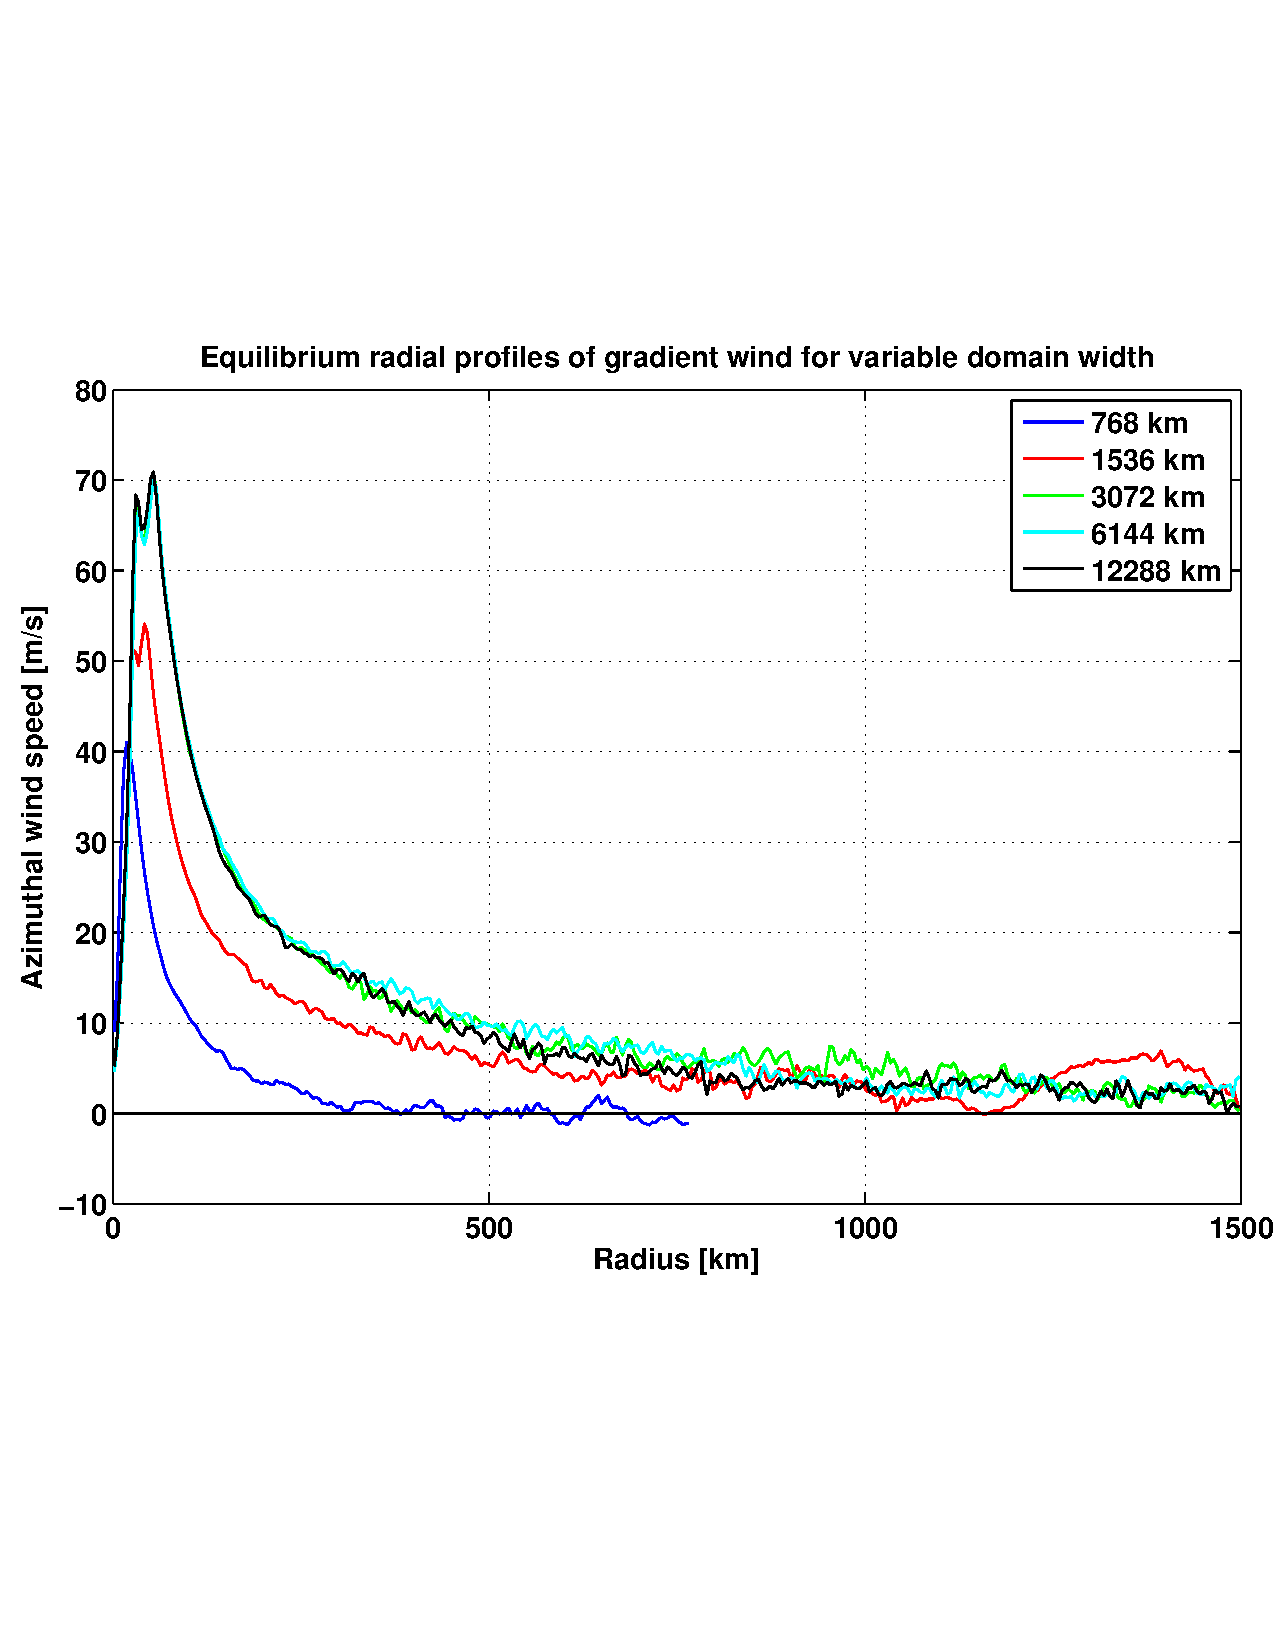
\includegraphics[width=19pc,angle=0]{FIGURES/Domain_size.pdf}
  \noindent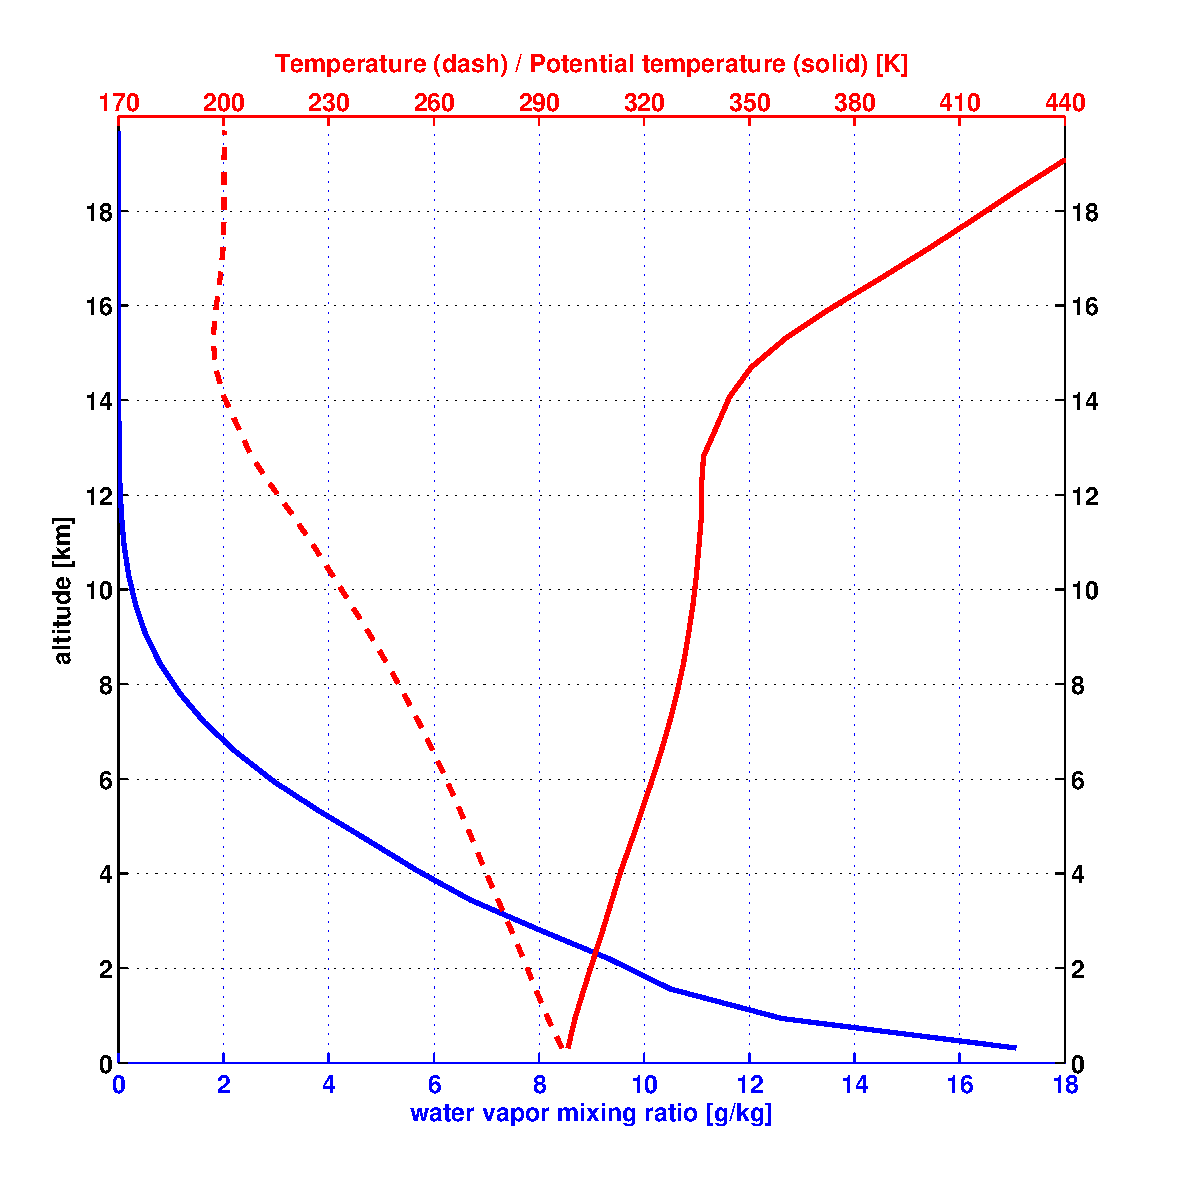
\includegraphics[width=10cm,height=10cm]{FIGURES_TC_RCE_equilibrium_v2.0/Fig0half_Sounding_ctrl.pdf}
\caption{Radiative-convective equilibrium vertical profile of temperature (red dashed), potential temperature (red solid), and water vapor mixing ratio (blue) for the Control simulation.}
\label{fig:ctrlsounding}
\end{figure}


\begin{figure}[h!]
\centering
%  \noindent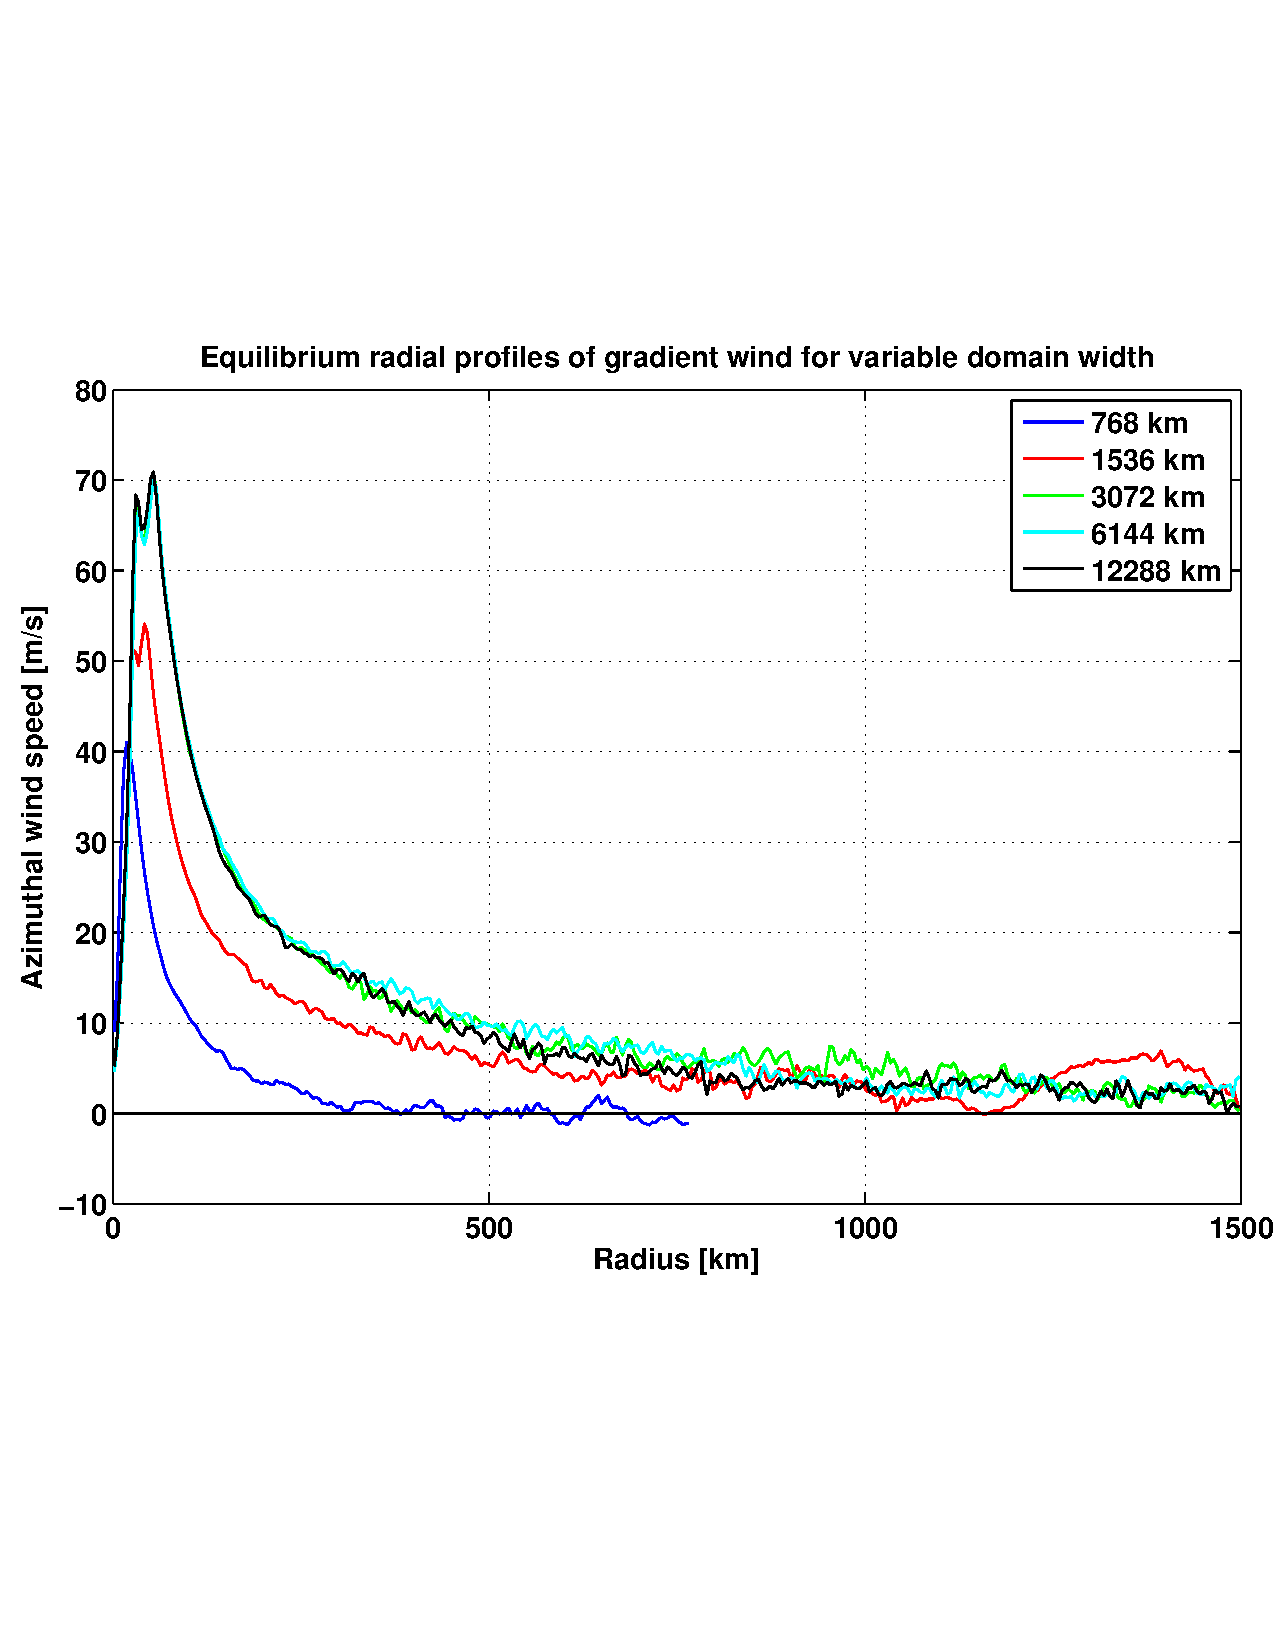
\includegraphics[width=19pc,angle=0]{FIGURES/Domain_size.pdf}
  \noindent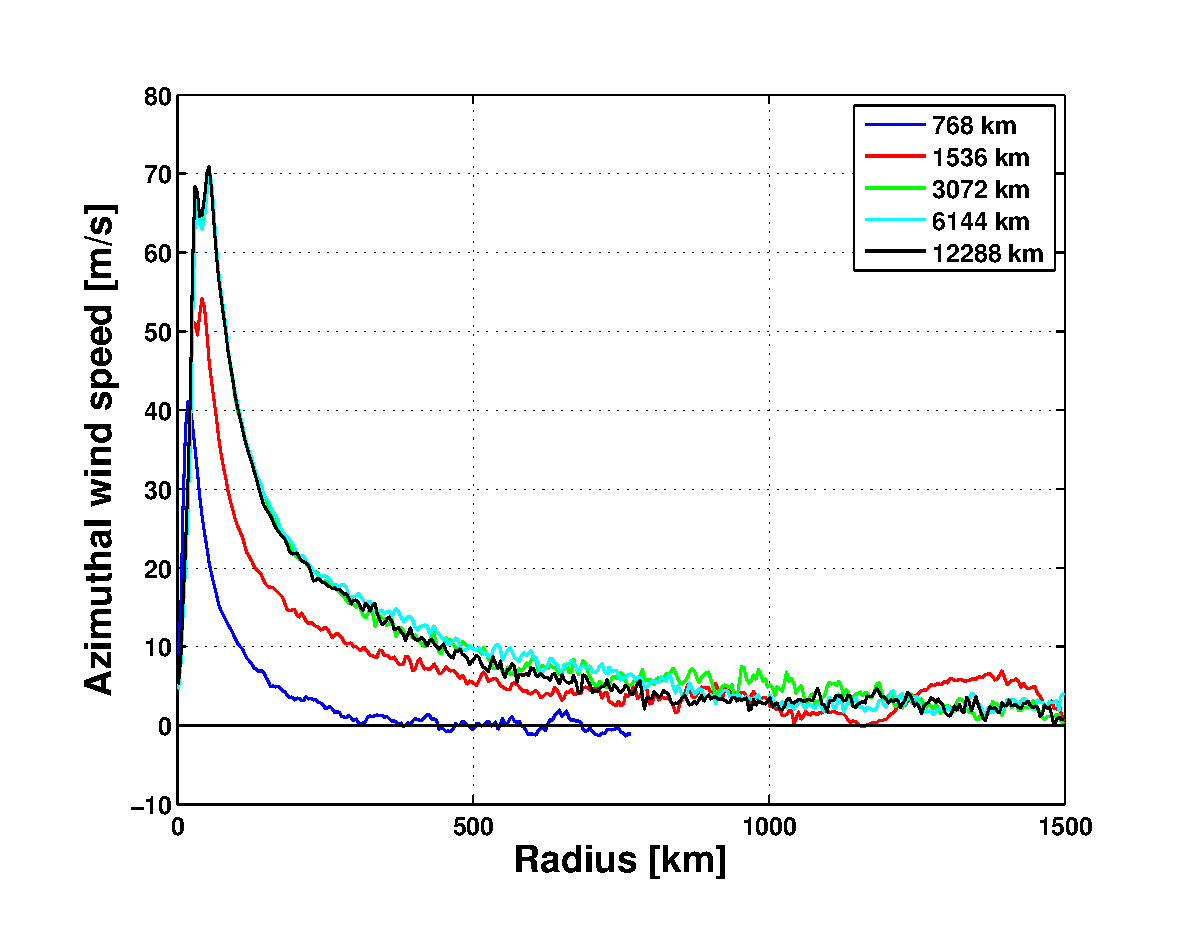
\includegraphics[width=15cm,height=10cm]{FIGURES_TC_RCE_equilibrium_v2.0/Fig1_Domain_size.pdf}
\caption{Equilibrium radial gradient wind profiles as a function of domain width.  Note the convergence in storm size beyond $L_{domain} \approx 3000 \; km$.}
\label{fig:domainsize}
\end{figure}

\begin{figure}[h!]
\centering
%  \noindent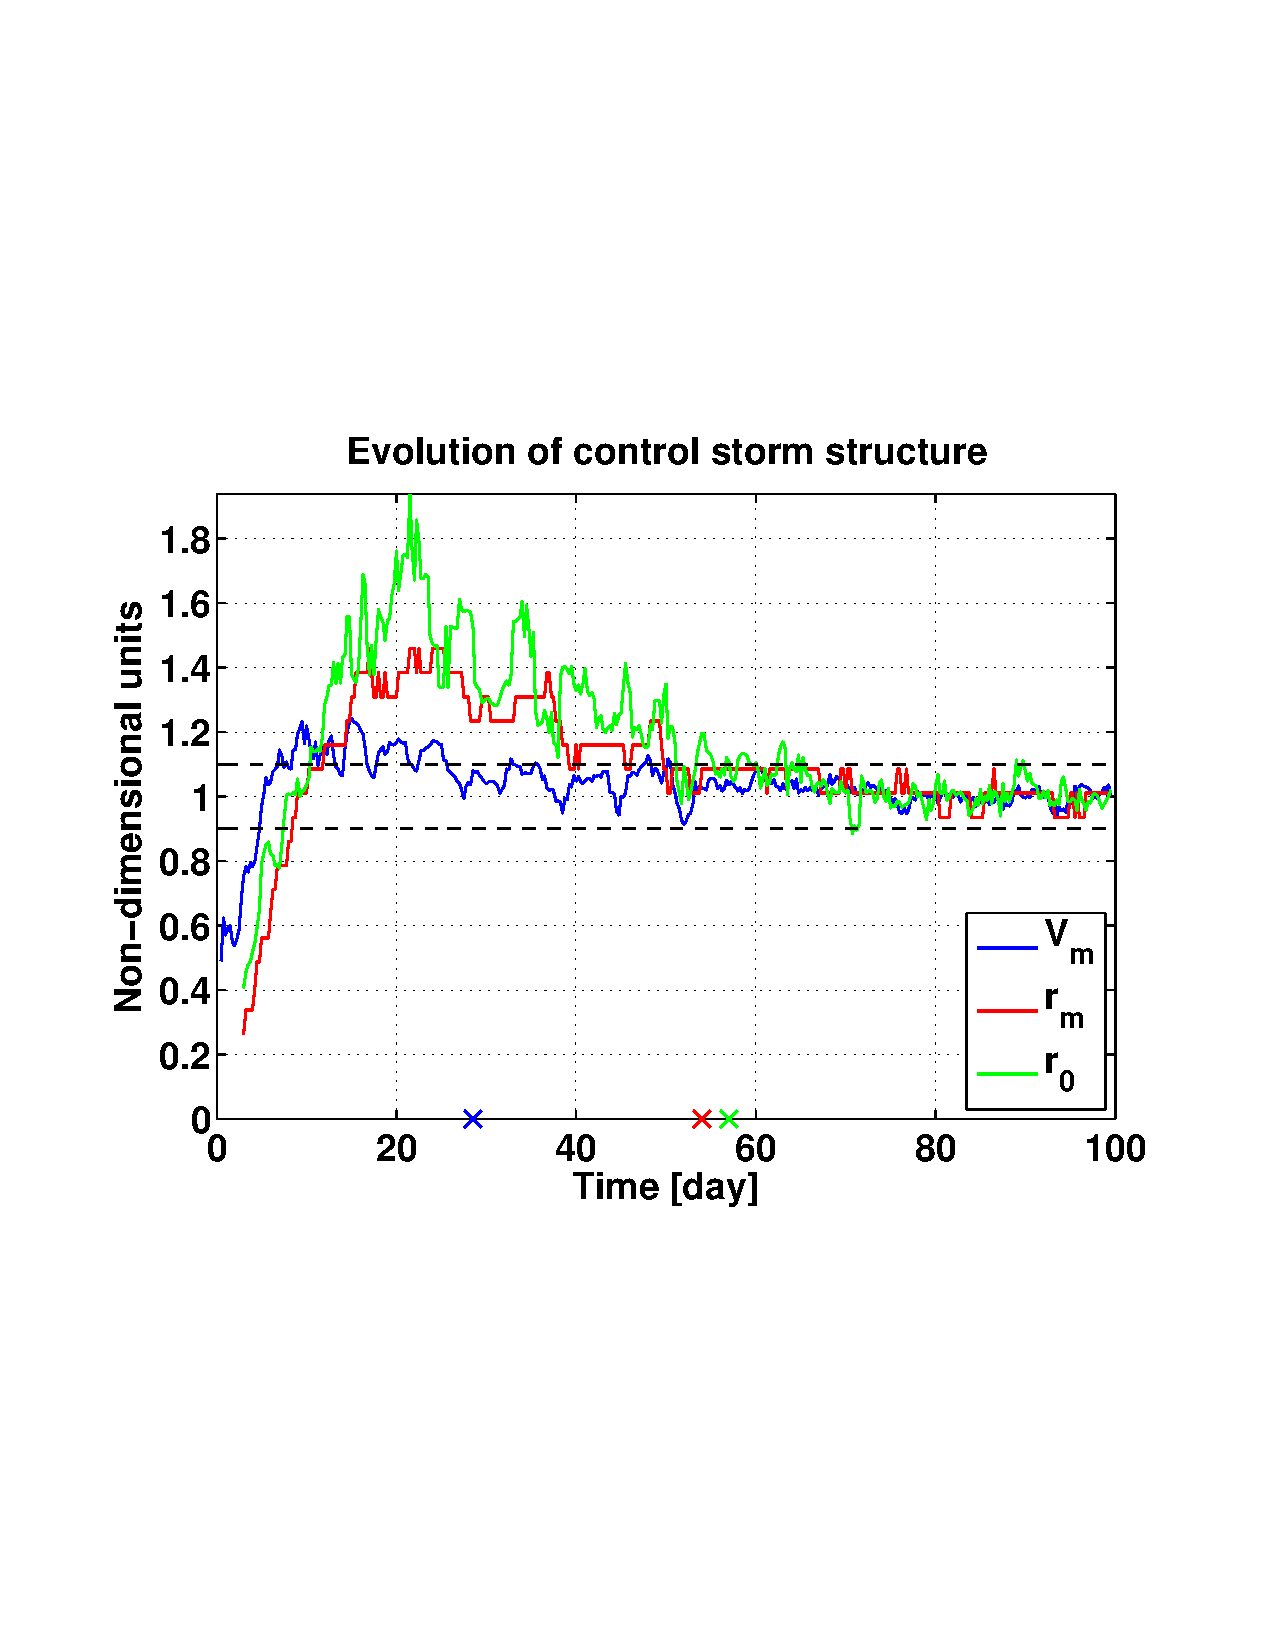
\includegraphics[width=19pc,angle=0]{FIGURES/Control_run.pdf}
  \noindent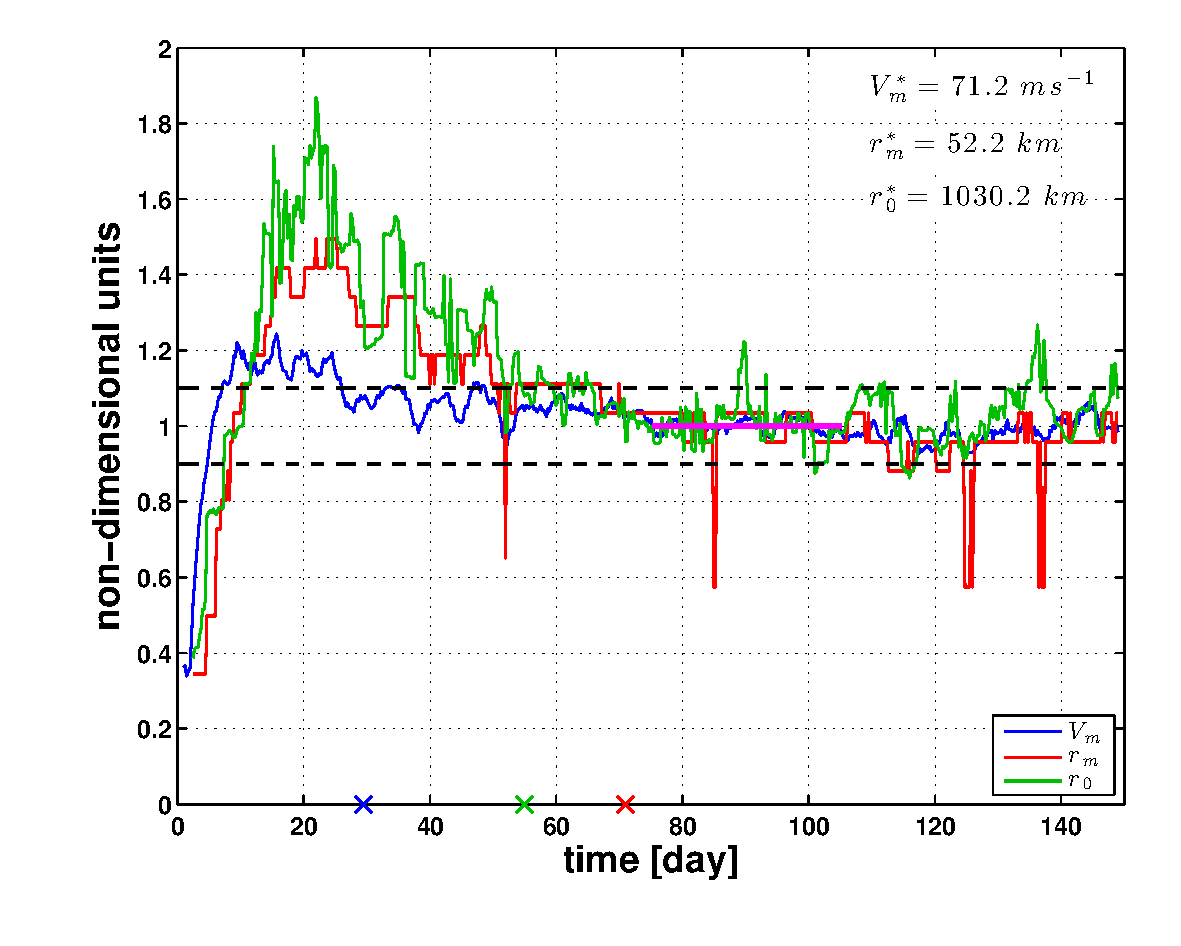
\includegraphics[width=15cm,height=10cm]{FIGURES_TC_RCE_equilibrium_v2.0/Fig2_Control_run.pdf}
\caption{For the Control simulation, time evolution of the 2-day running mean $V_m$, $r_m$, and $r_0$ normalized by their respective equilibrium values (upper-right corner). For this simulation, $V^*_p =  92 \; ms^{-1}$ and $f = 5*10^{-5} \; s^{-1}$. Pink line denotes 30-day period used for equilibrium calculation, and black dashed lines denote $\pm10\%$ of the equilibrium value. Markers along the x-axis denote estimated time-scales to equilibration; see text for details.}
\label{fig:timeseries}.
\end{figure}

\begin{figure}[h!]
\centering
%  \noindent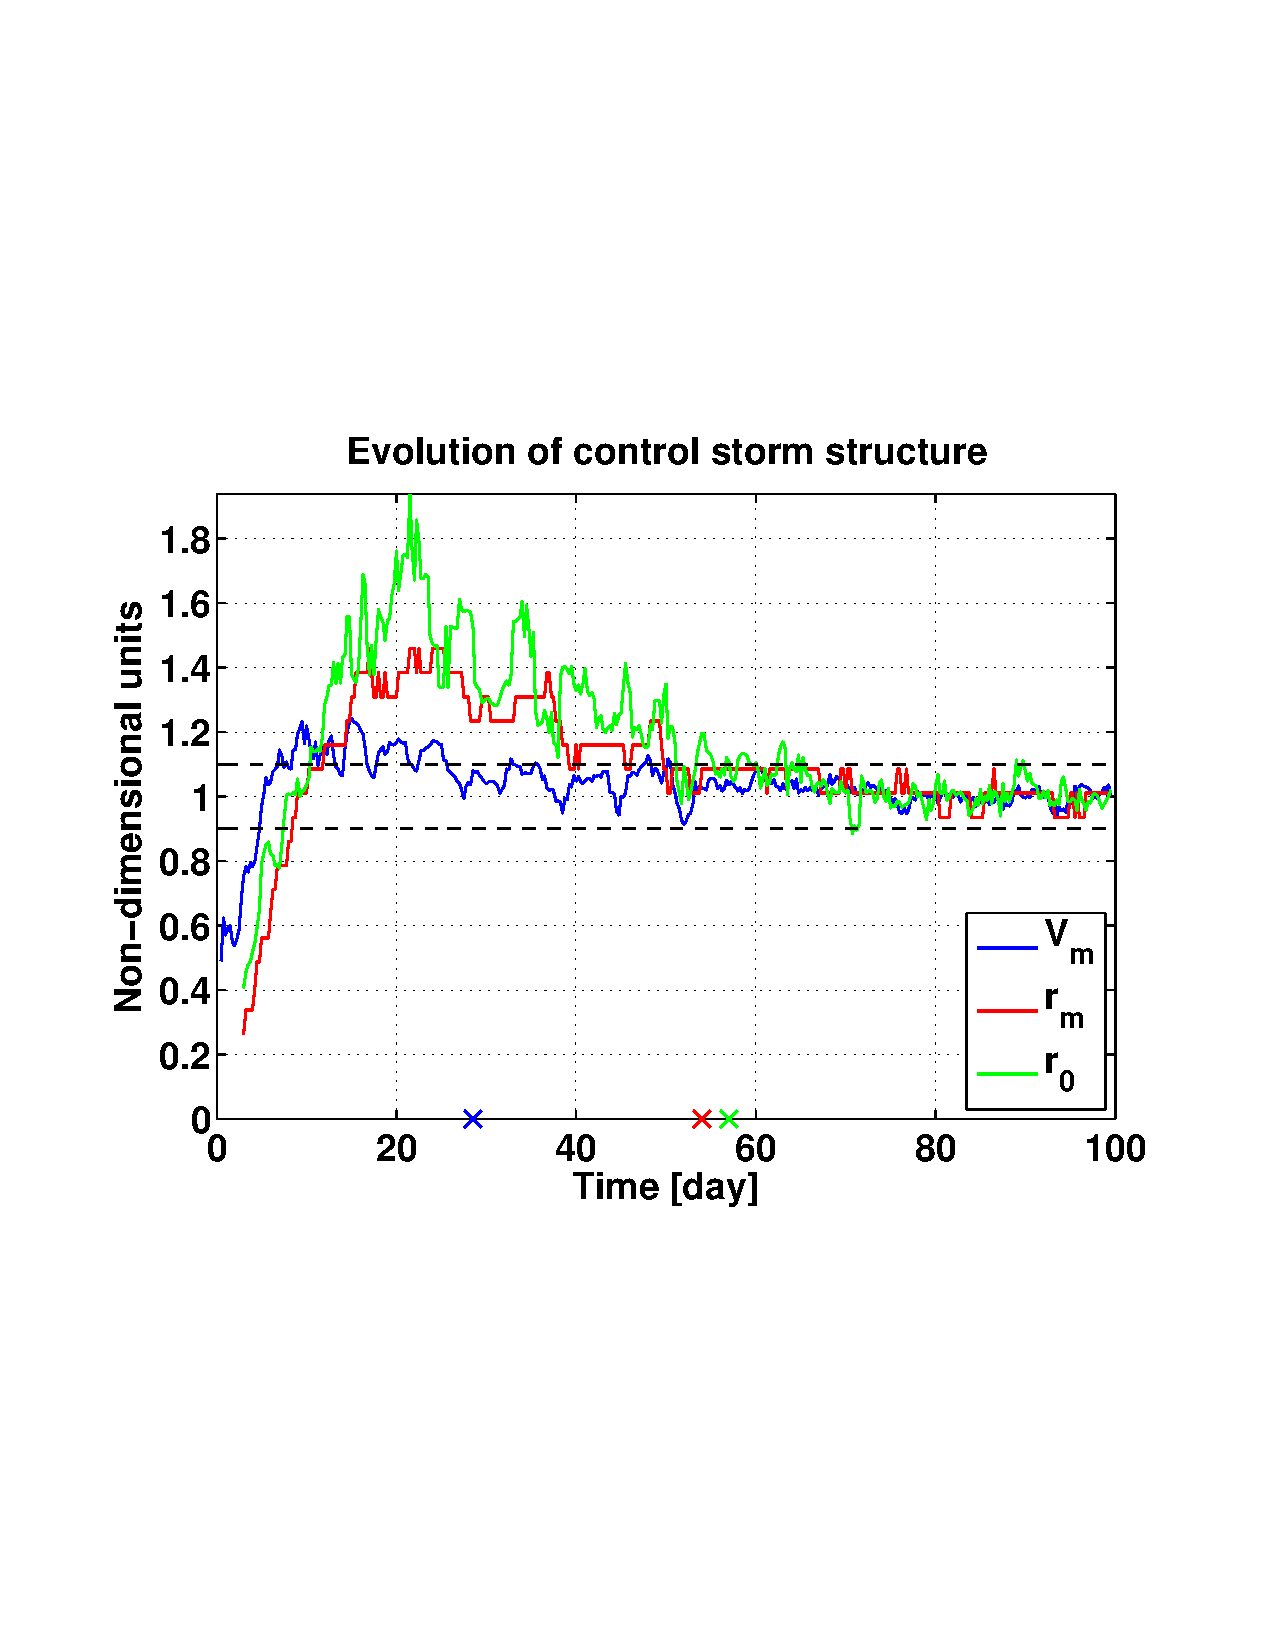
\includegraphics[width=19pc,angle=0]{FIGURES/Control_run.pdf}
  \noindent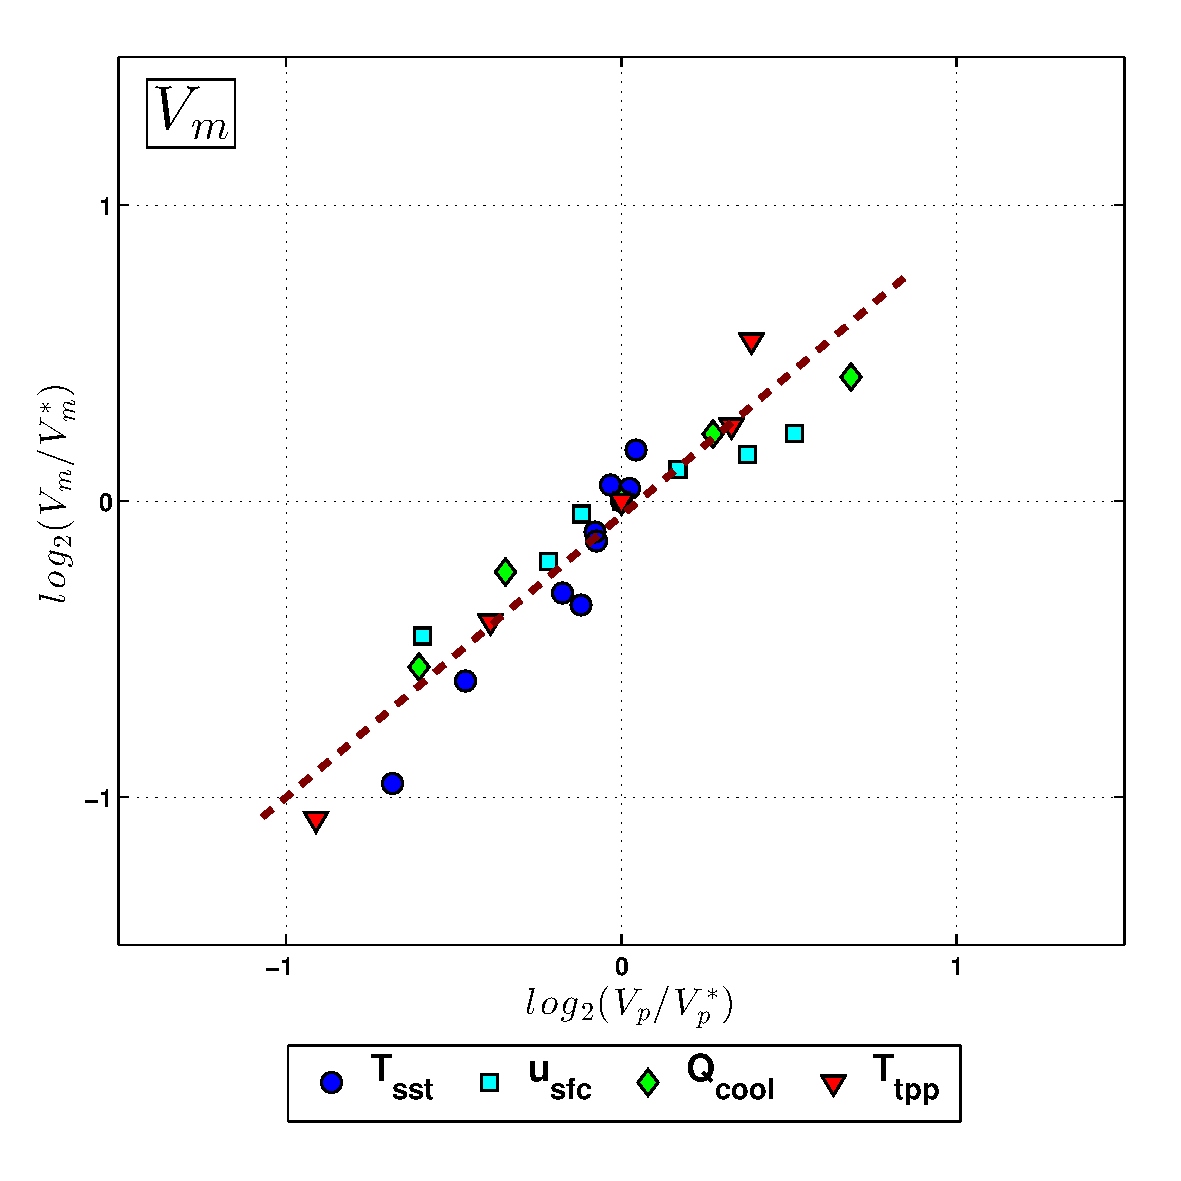
\includegraphics[width=10cm,height=10cm]{FIGURES_TC_RCE_equilibrium_v2.0/Fig3_MPI_collapse_V.pdf}
\caption{Scaling of the equilibrium value of $V_m$ (ordinate) with the potential intensity (abscissa). Both quantities are normalized by their respective control values denoted by an asterisk ($*$; $V^*_p = 93 \; ms^{-1}$). Colored shape denotes the input parameter varied from among the four parameters on which the potential intensity depends (Eq. \eqref{eq:vpot3}). Scaling is shown in base-2 log-log space, such that a 1-unit increase (decrease) represents doubling (having). Grey bars indicate the range of variability of the 30-day running mean after day 60.}
\label{fig:mpicollapse_V}
\end{figure}

\begin{figure}[h!]
\centering
%  \noindent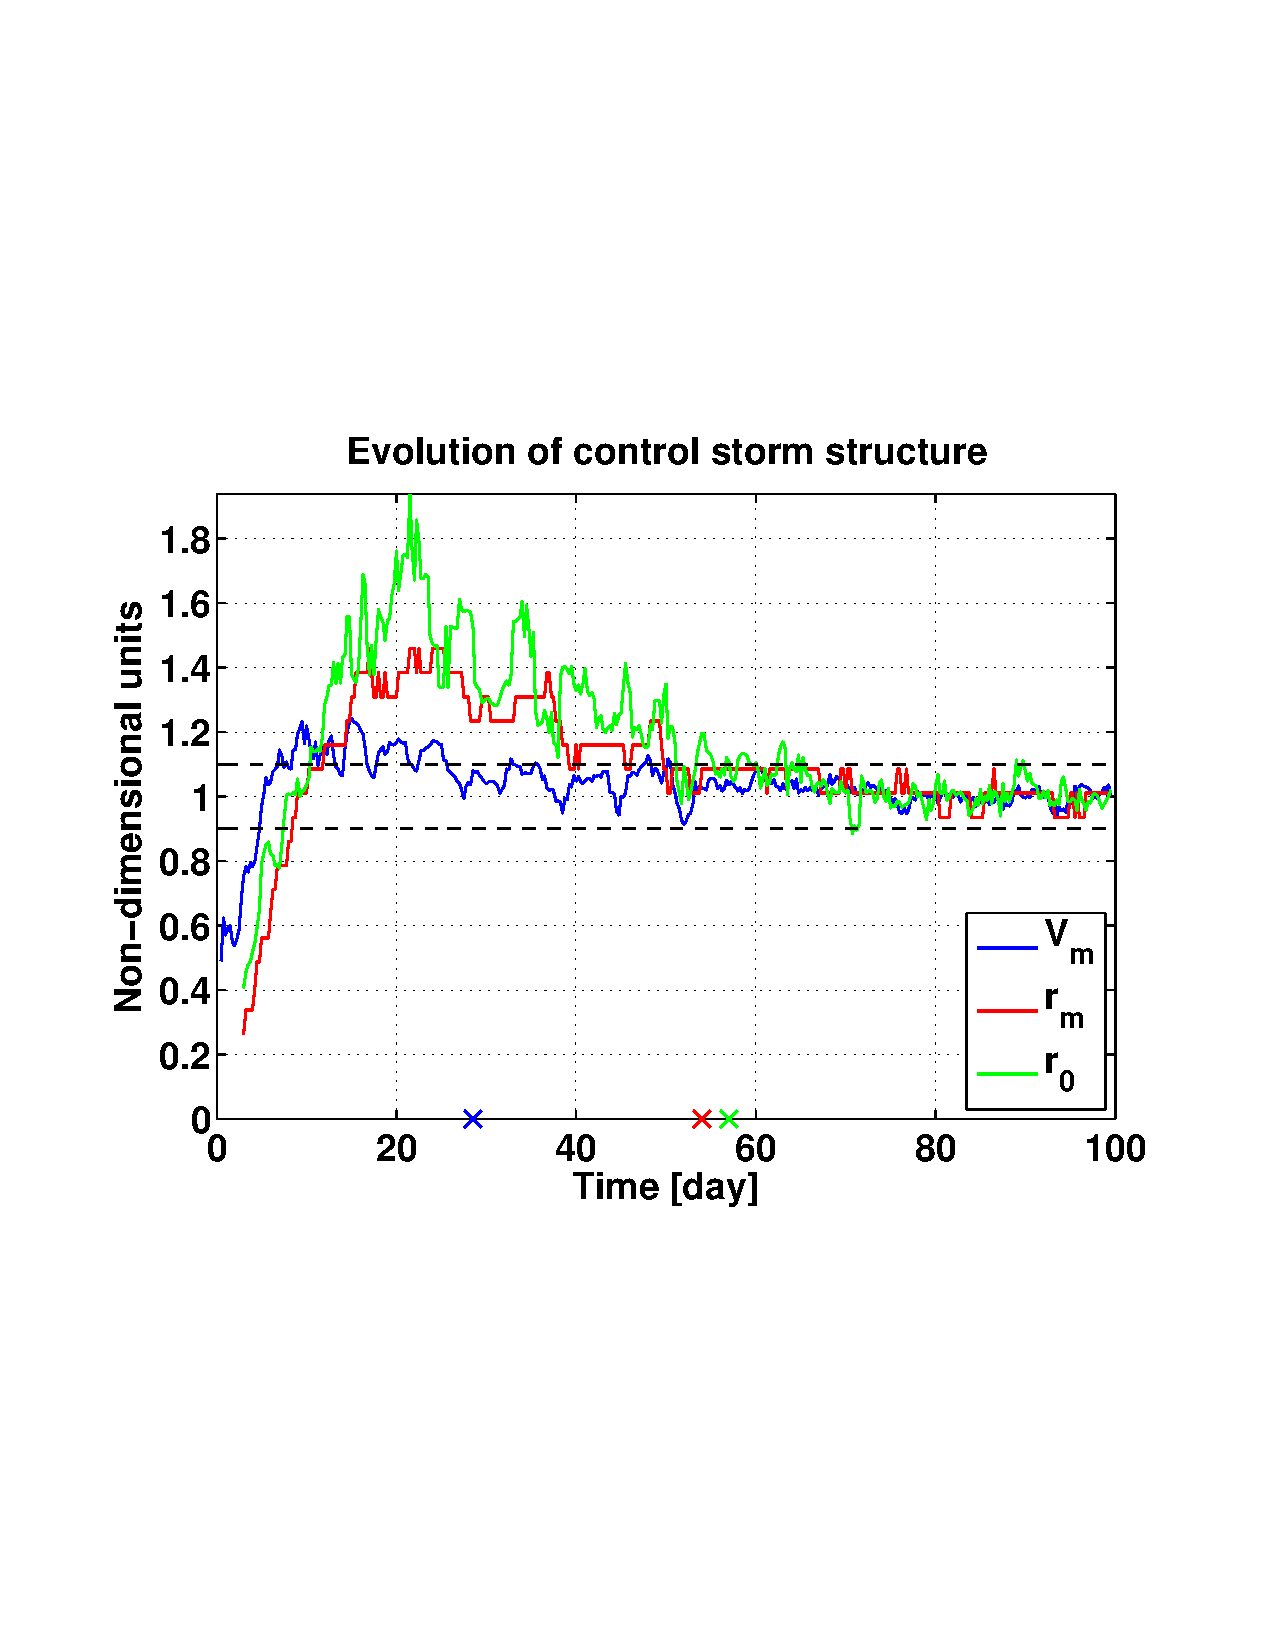
\includegraphics[width=19pc,angle=0]{FIGURES/Control_run.pdf}
  \noindent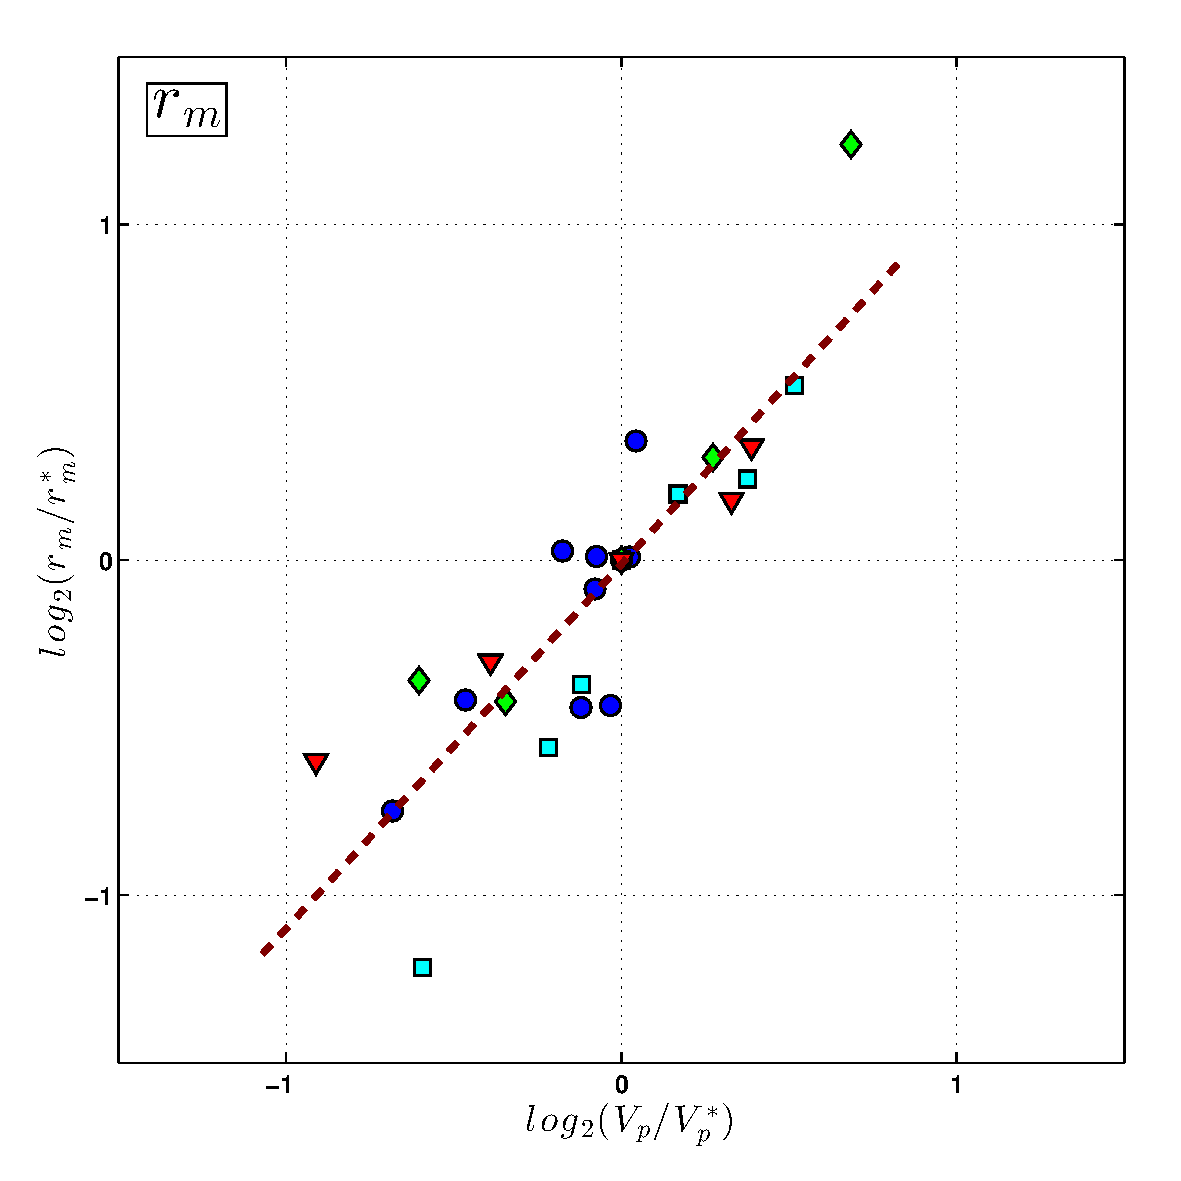
\includegraphics[width=10cm,height=9cm]{FIGURES_TC_RCE_equilibrium_v2.0/Fig4a_MPI_collapse_rm.pdf}
  
  \noindent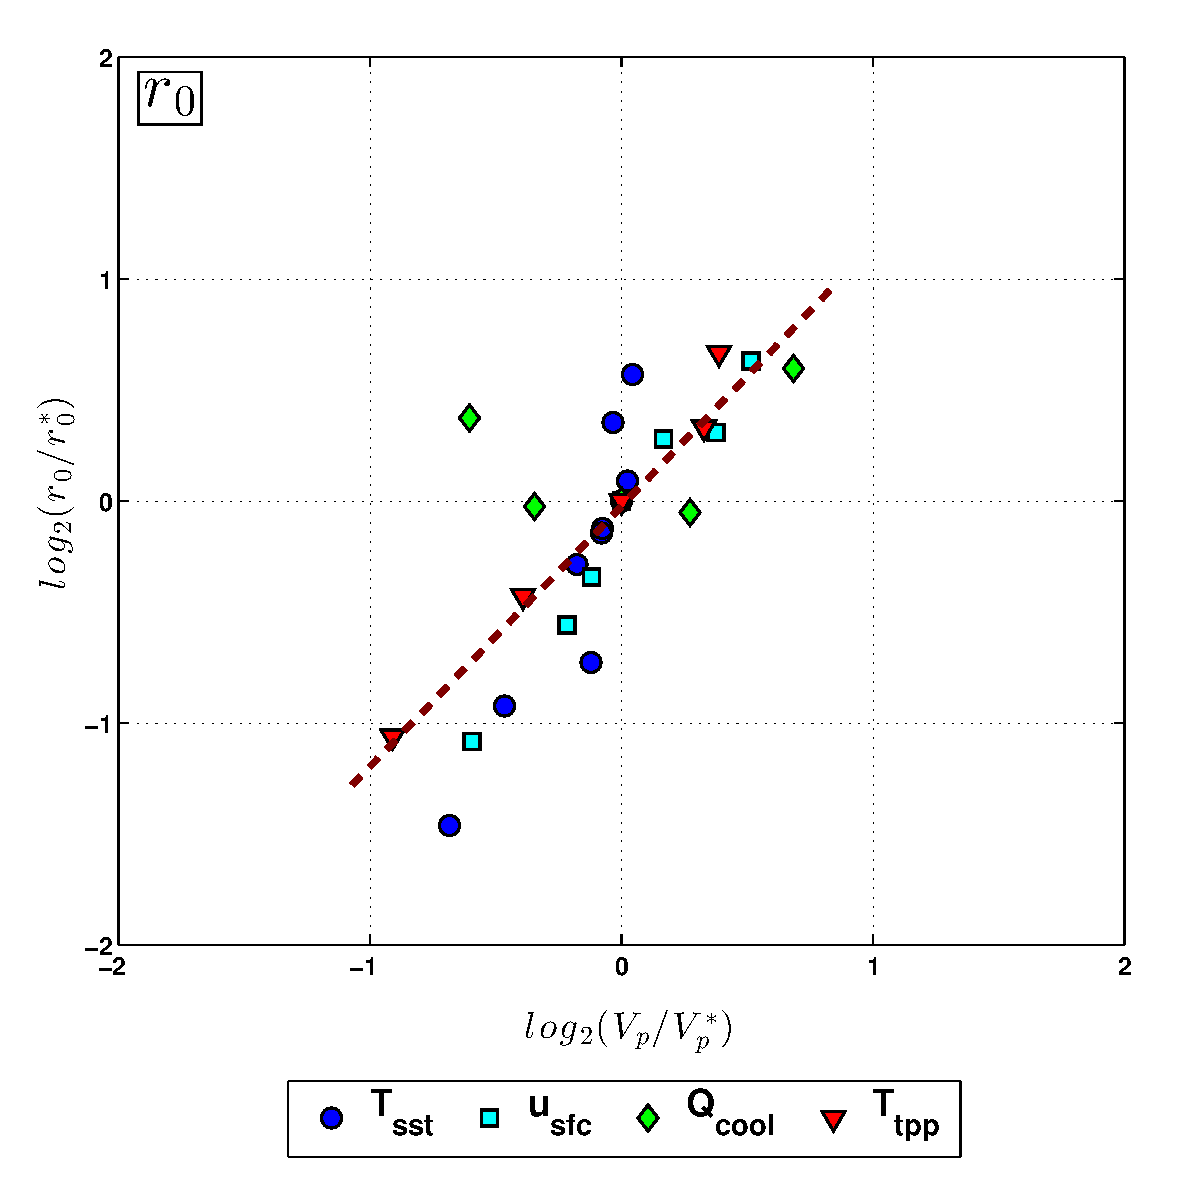
\includegraphics[width=10cm,height=10cm]{FIGURES_TC_RCE_equilibrium_v2.0/Fig4b_MPI_collapse_r0.pdf}
\caption{As in Figure \ref{fig:mpicollapse_V}, but for $r_m$ (top) and $r_{0}$ (bottom).}
\label{fig:mpicollapse_r}
\end{figure}

\begin{figure}[h!]
\centering
%  \noindent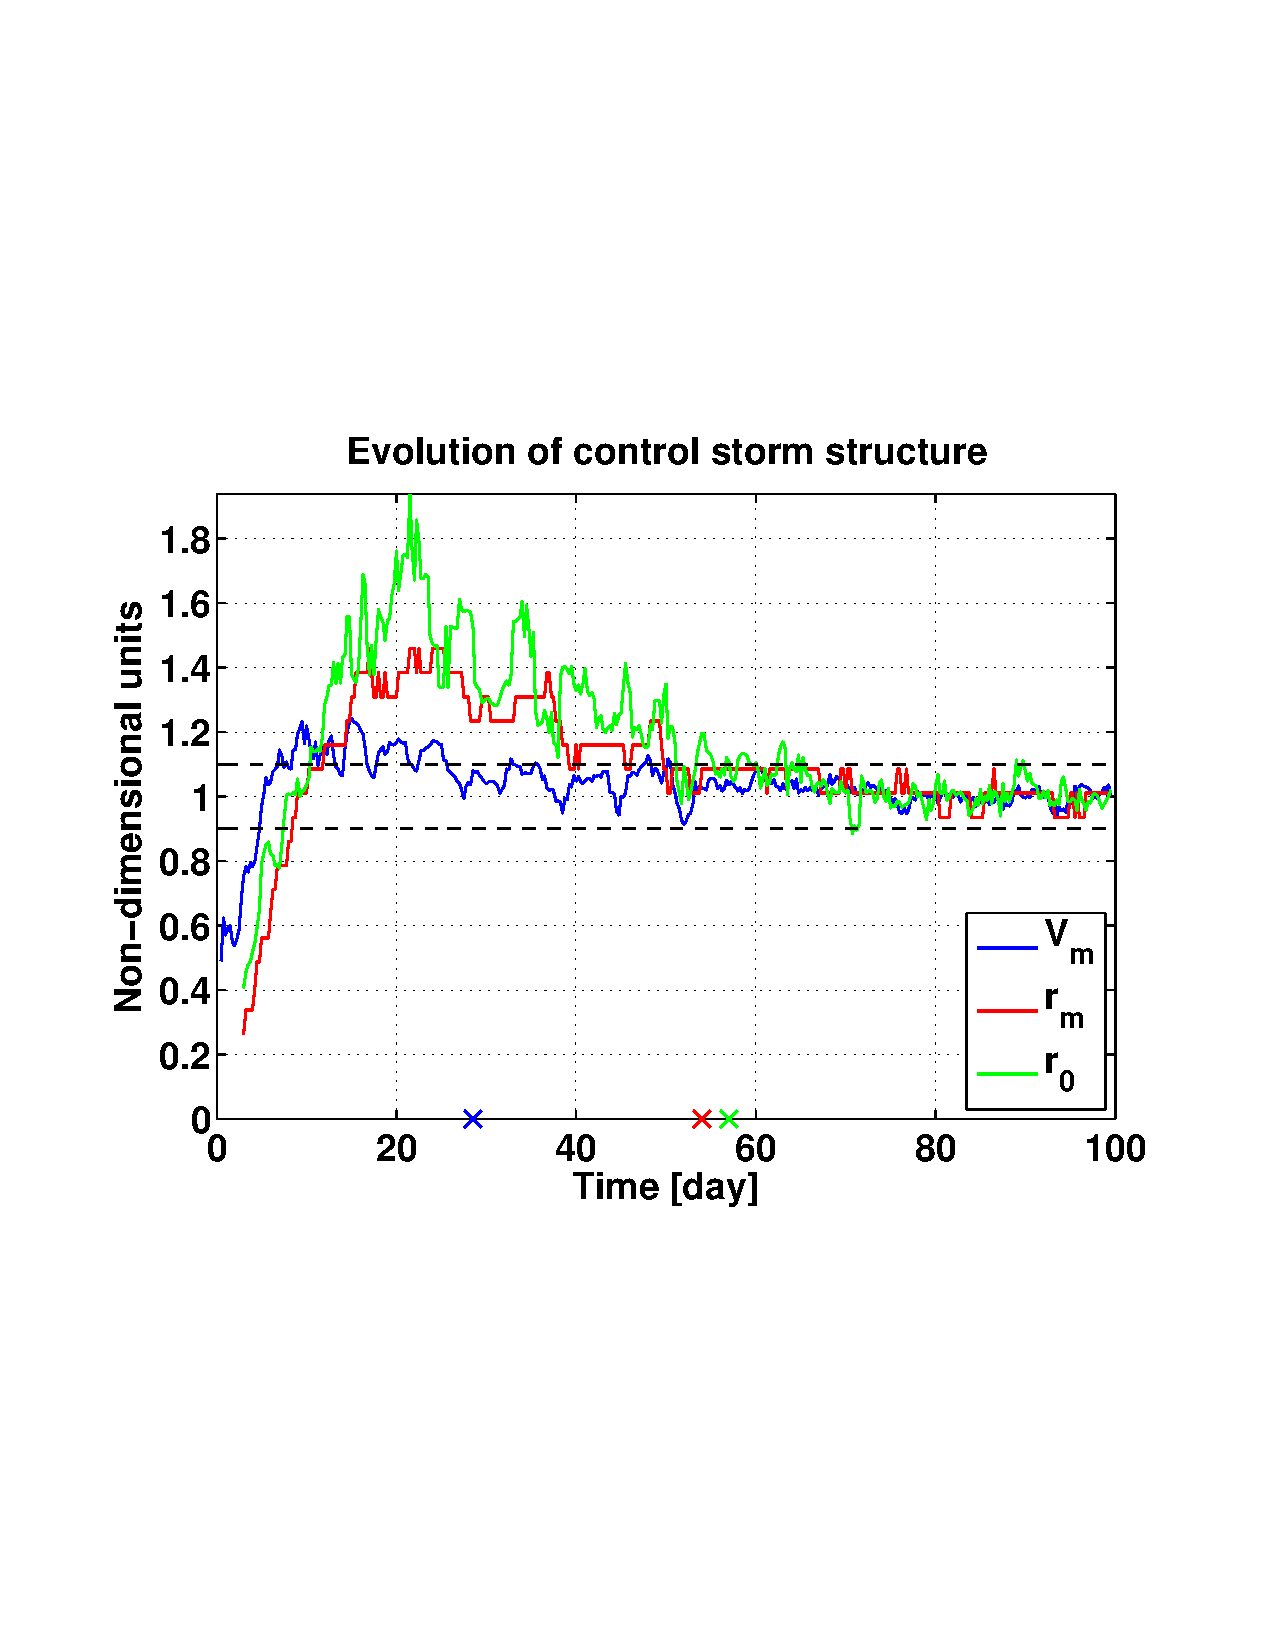
\includegraphics[width=19pc,angle=0]{FIGURES/Control_run.pdf}
  \noindent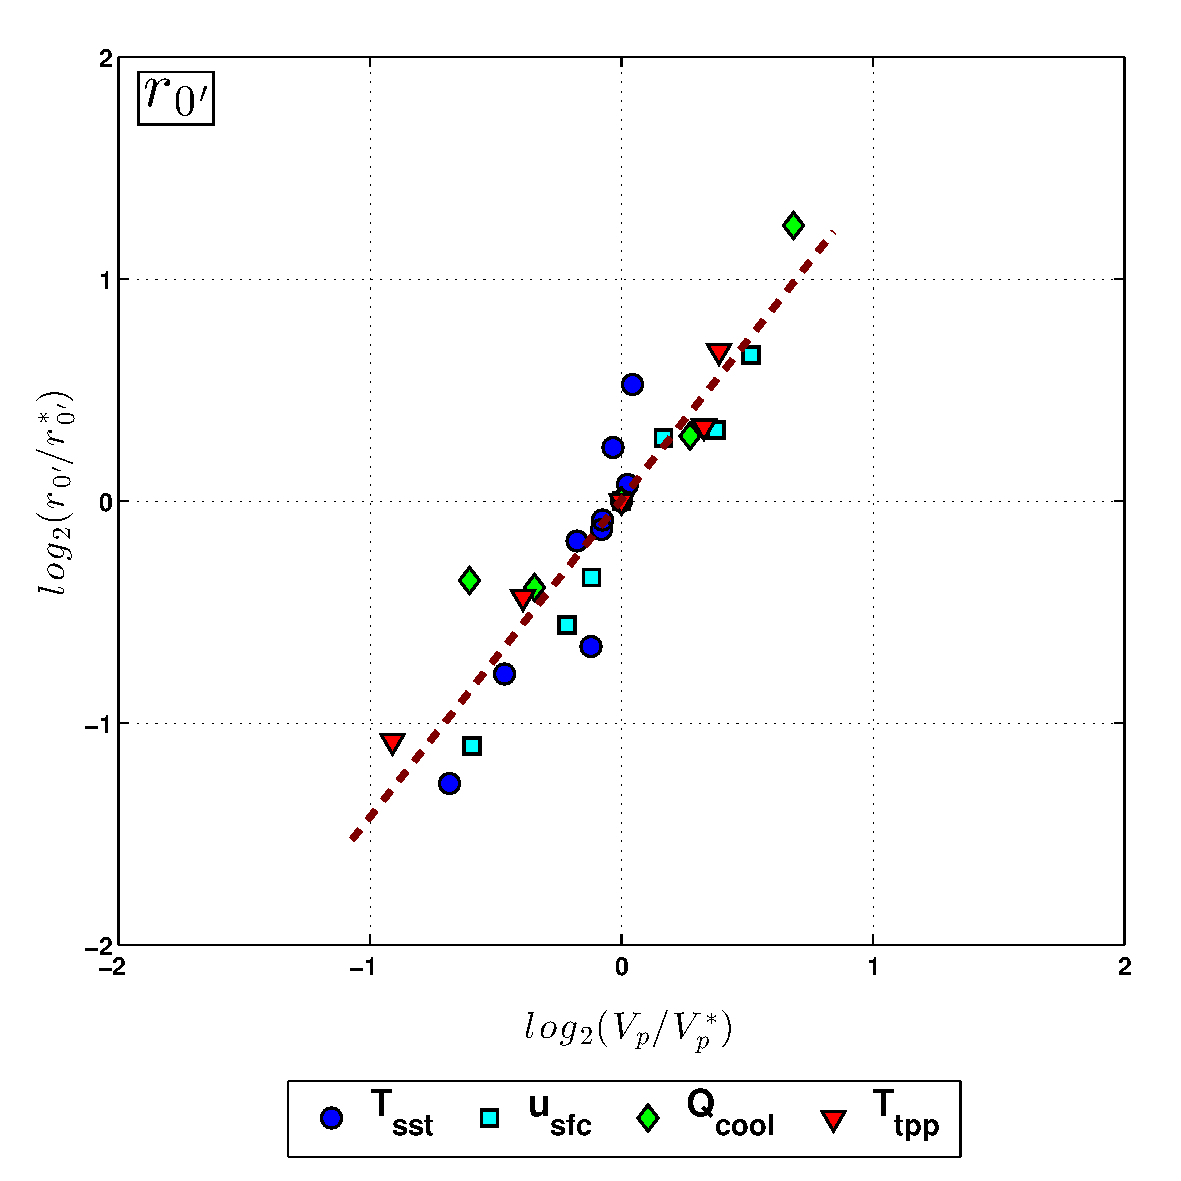
\includegraphics[width=10cm,height=10cm]{FIGURES_TC_RCE_equilibrium_v2.0/Fig5_MPI_collapse_r0ctrlwcool.pdf}
\caption{As in Figure \ref{fig:mpicollapse_r}, but where $r_{0'}$ is $r_0$ calculated from \eqref{eq:radsub} using the control value of $w_{cool}$.}
\label{fig:mpicollapse_r0ctrlwcool}
\end{figure}

\begin{figure}[h!]
\centering
%  \noindent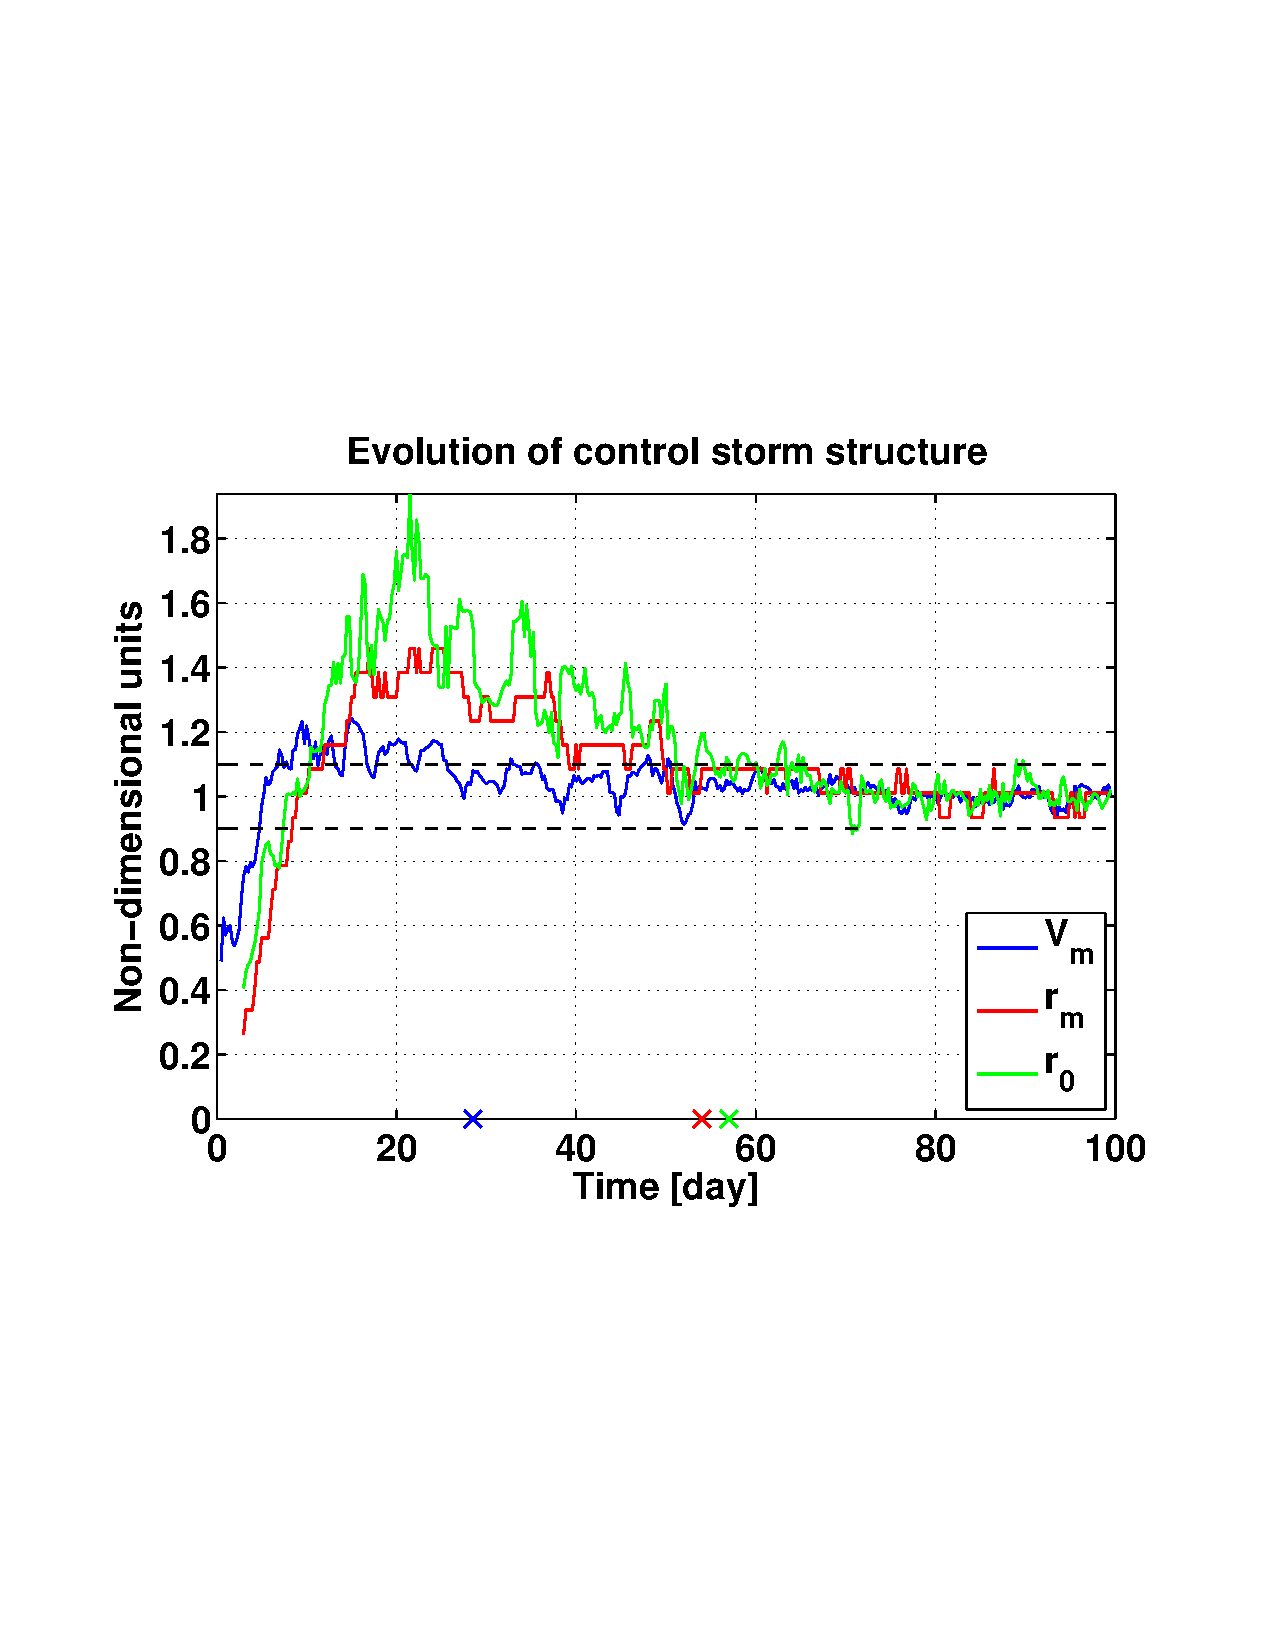
\includegraphics[width=19pc,angle=0]{FIGURES/Control_run.pdf}
  \noindent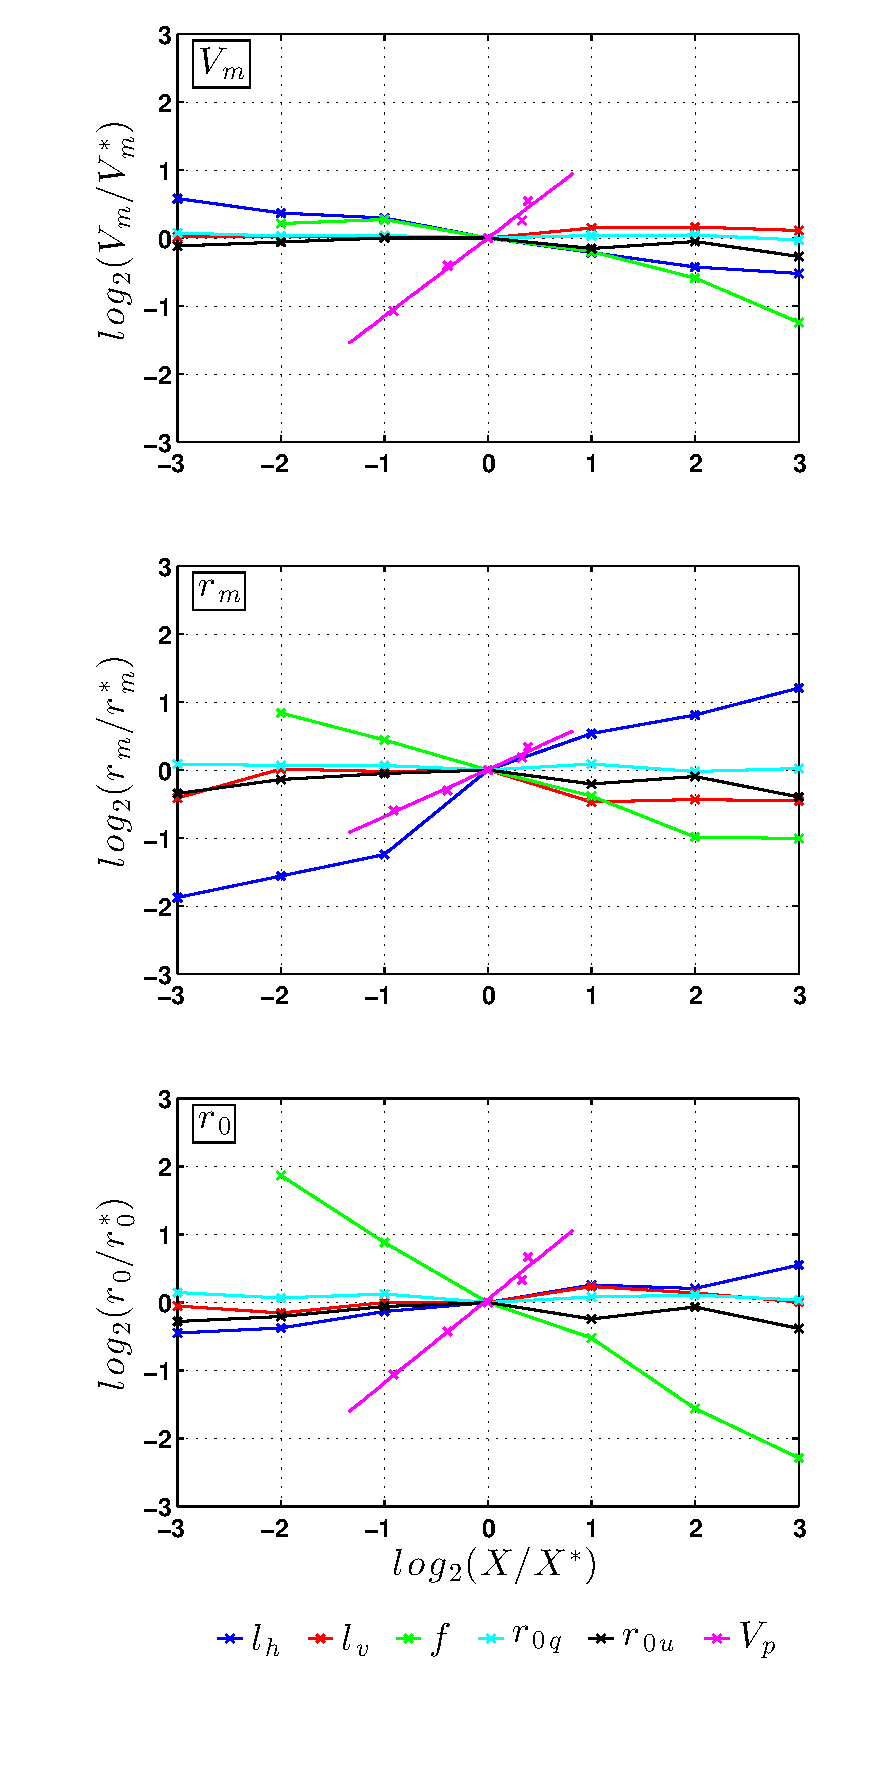
\includegraphics[width=8cm,height=20cm]{FIGURES_TC_RCE_equilibrium_v2.0/Fig6_Dimensional_scaling.pdf}
\caption{Scaling of the equilibrium value of each structural variable (ordinate) with relevant dimensional parameters, $X$ (absicssa). All quantities are normalized by their respective control values denoted by an asterisk ($*$). Plot layout as in Figure \ref{fig:mpicollapse_V}.}
\label{fig:dimscaling}
\end{figure}

\begin{figure}[h!]
\centering
%  \noindent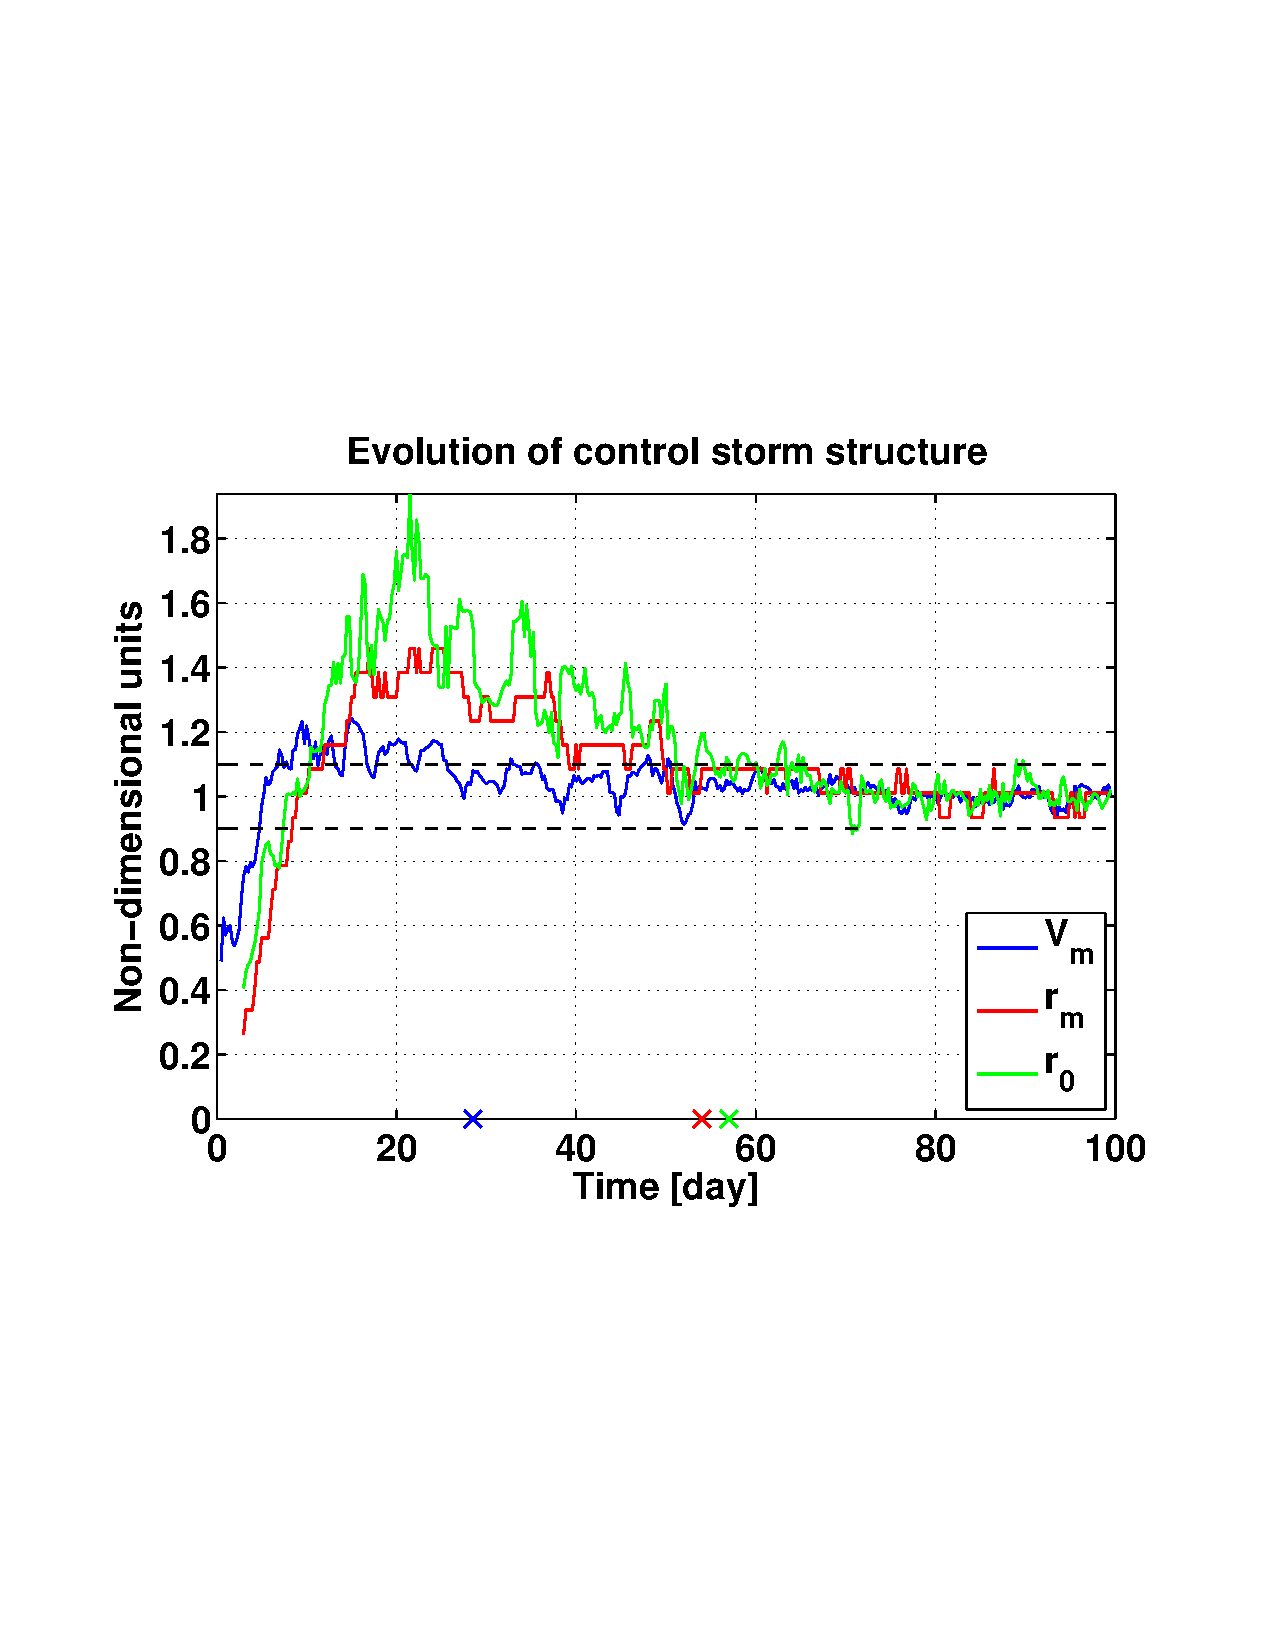
\includegraphics[width=19pc,angle=0]{FIGURES/Control_run.pdf}
  \noindent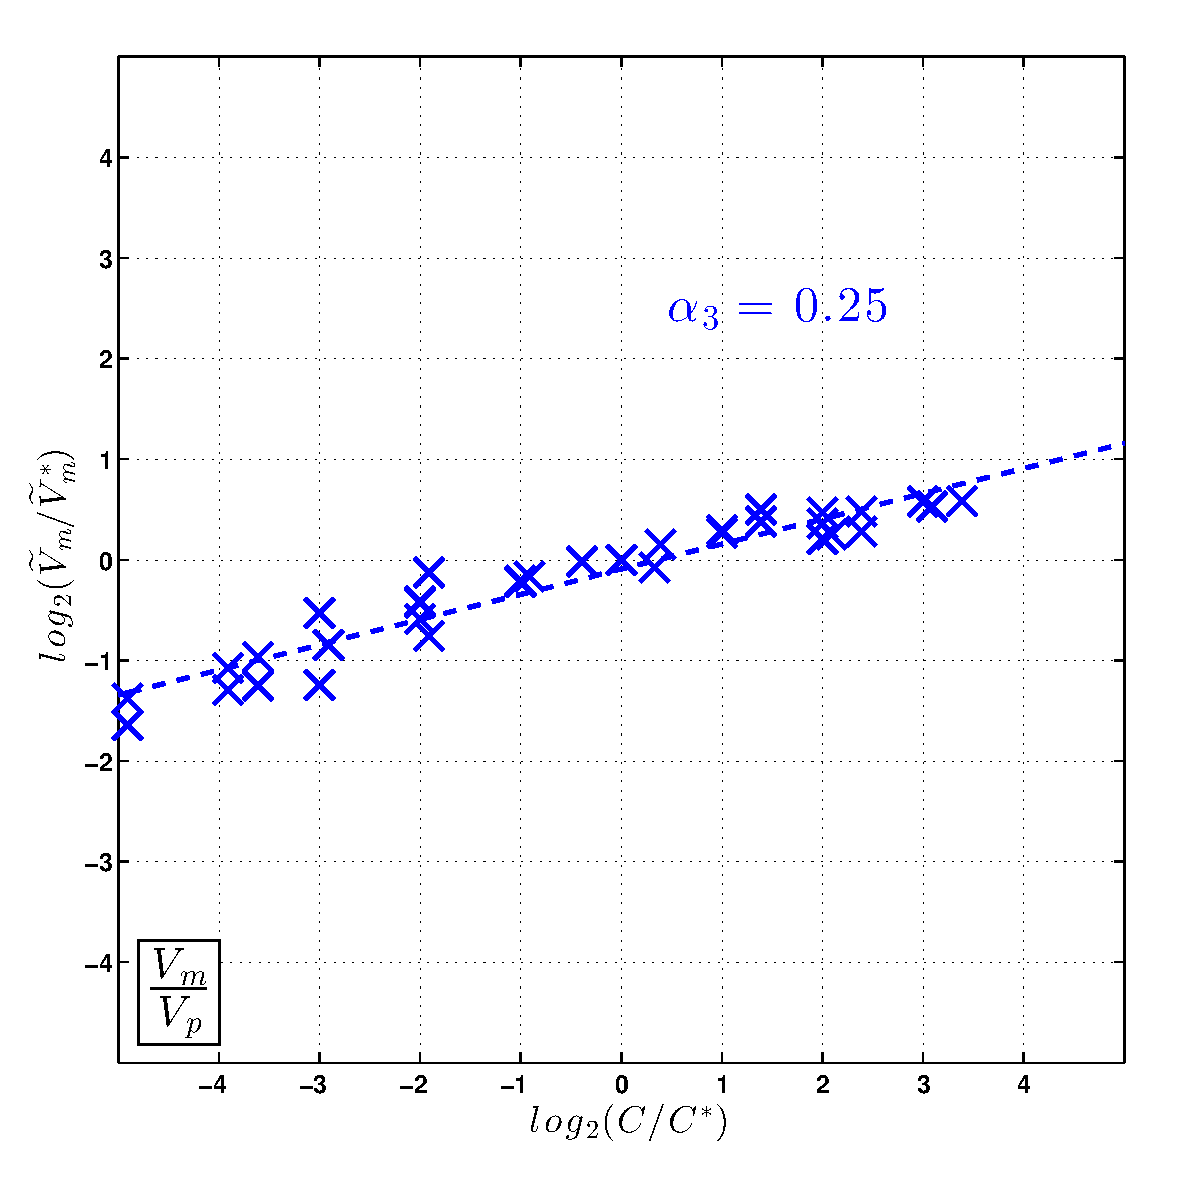
\includegraphics[width=6cm,height=6cm]{FIGURES_TC_RCE_equilibrium_v2.0/Fig7a_Nondimensional_scaling_V.pdf}
  
  \noindent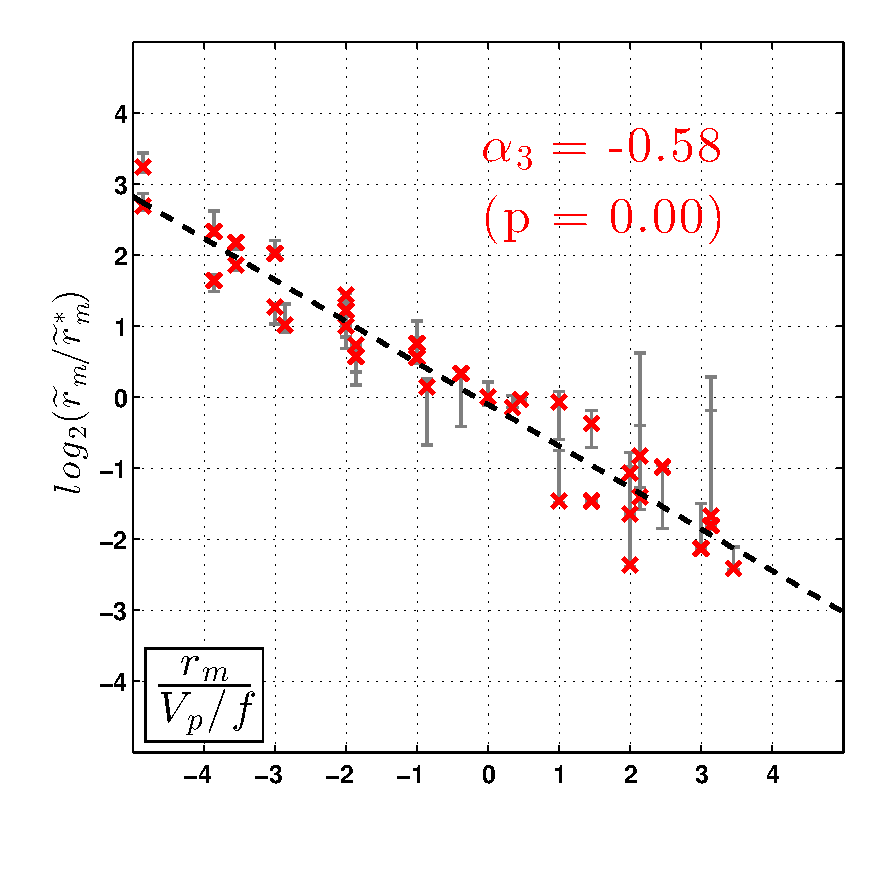
\includegraphics[width=6cm,height=6cm]{FIGURES_TC_RCE_equilibrium_v2.0/Fig7b_Nondimensional_scaling_rm.pdf}
  
  \noindent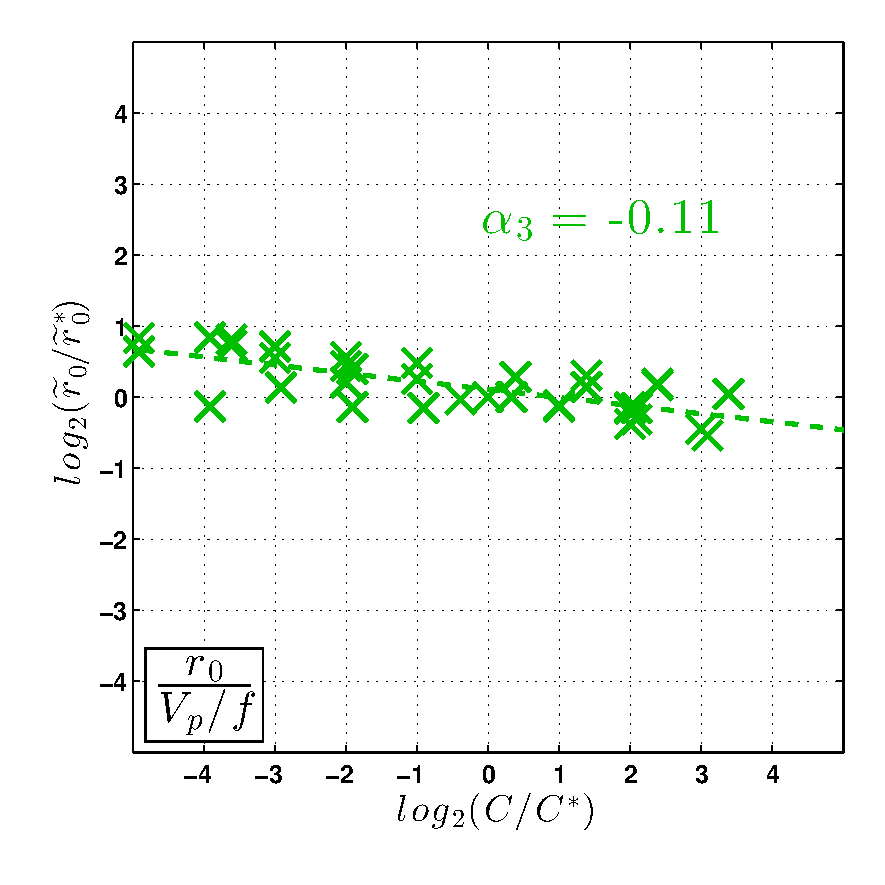
\includegraphics[width=6cm,height=6cm]{FIGURES_TC_RCE_equilibrium_v2.0/Fig7c_Nondimensional_scaling_r0.pdf}

\caption{Scaling of the equilibrium values of the non-dimensionalized structural variable $V_m$ (top), $r_m$ (middle), and $r_0$ (bottom) with the non-dimensional number $C = \frac{V_p}{fl_h}$; see text for details. All quantities are normalized by their respective control values denoted by an asterisk ($*$; $C^* = 1220$). Plot layout as in Figure \ref{fig:mpicollapse_V}.  Best-fit linear regressions plotted (dash); linearly-regressed slopes, corresponding to the estimated power-law scaling exponent in \eqref{eq:buckpipowerlaw}, and associated p-values listed within. For $V_m$, a logarithmic regression is also shown (dash-dot).}
\label{fig:nondimscaling}
\end{figure}

\begin{figure}[h!]
\centering
%  \noindent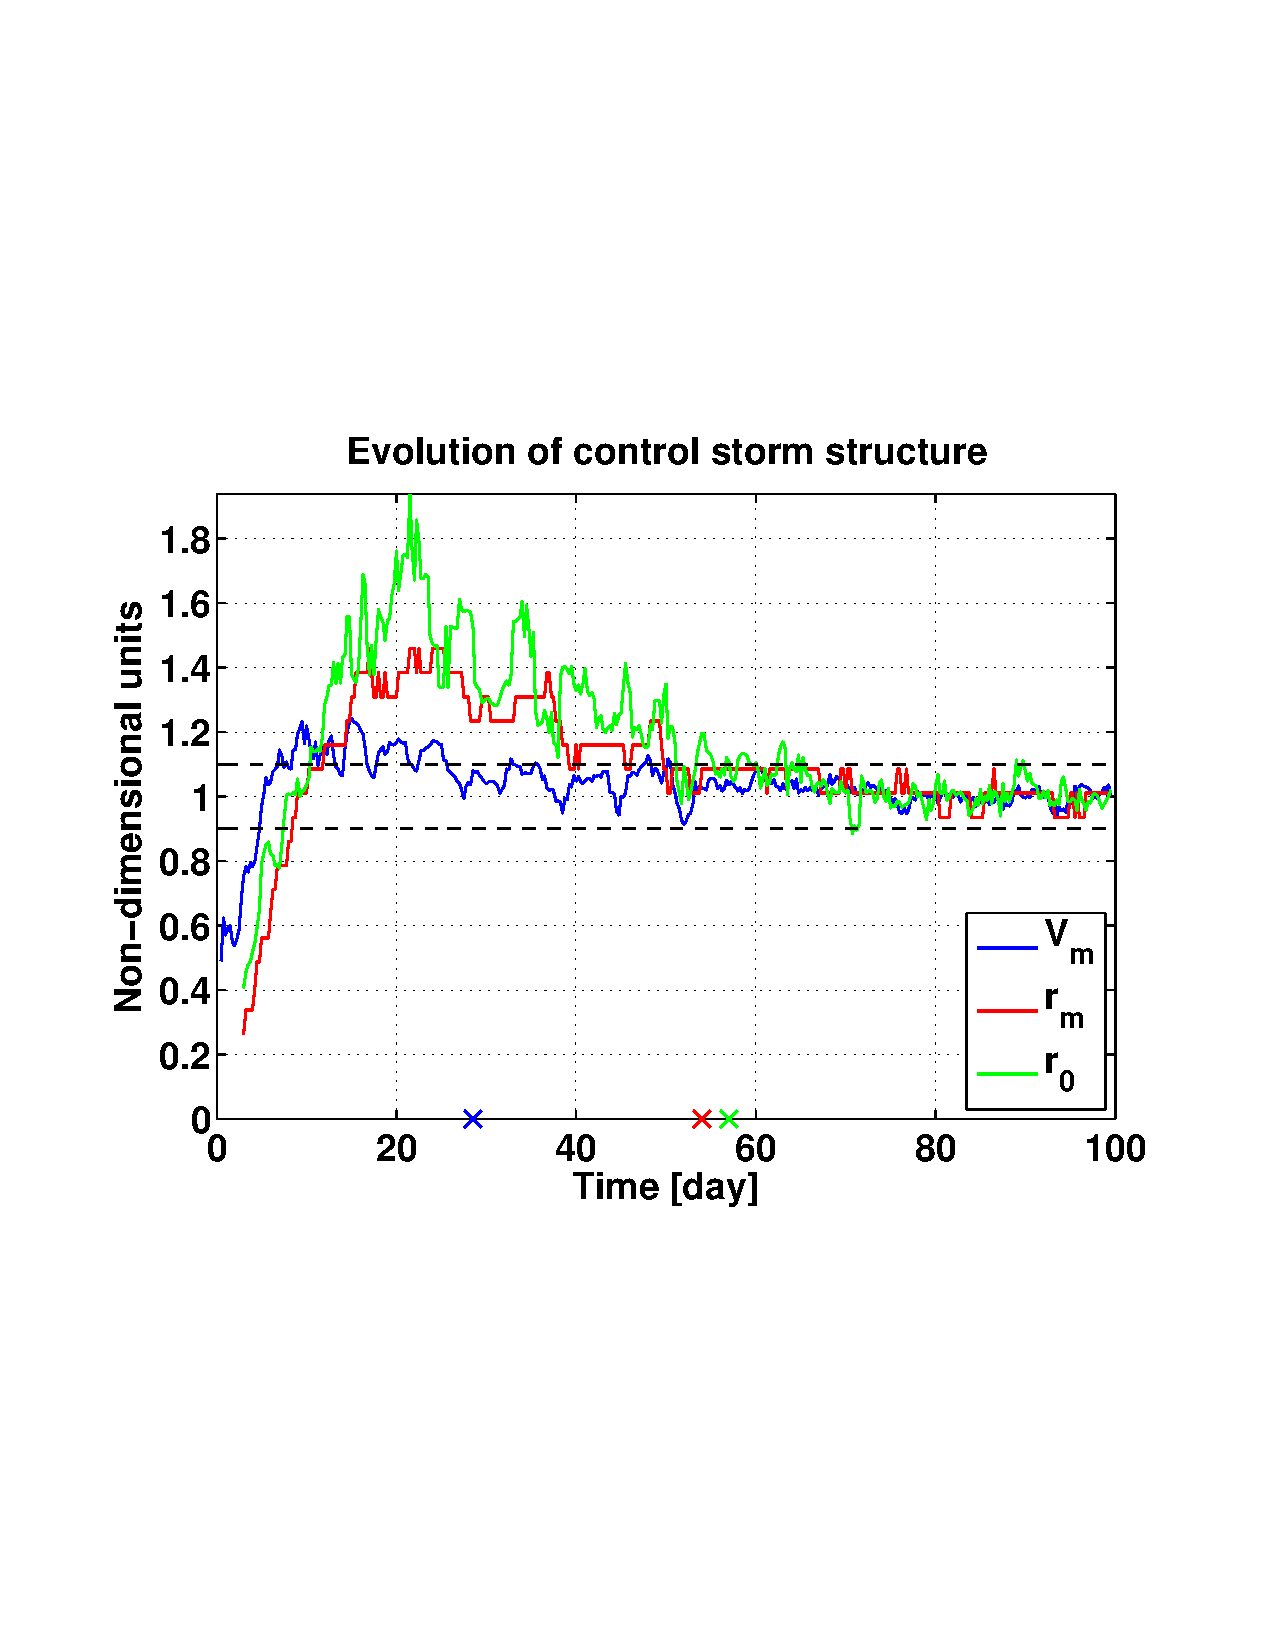
\includegraphics[width=19pc,angle=0]{FIGURES/Control_run.pdf}
  \noindent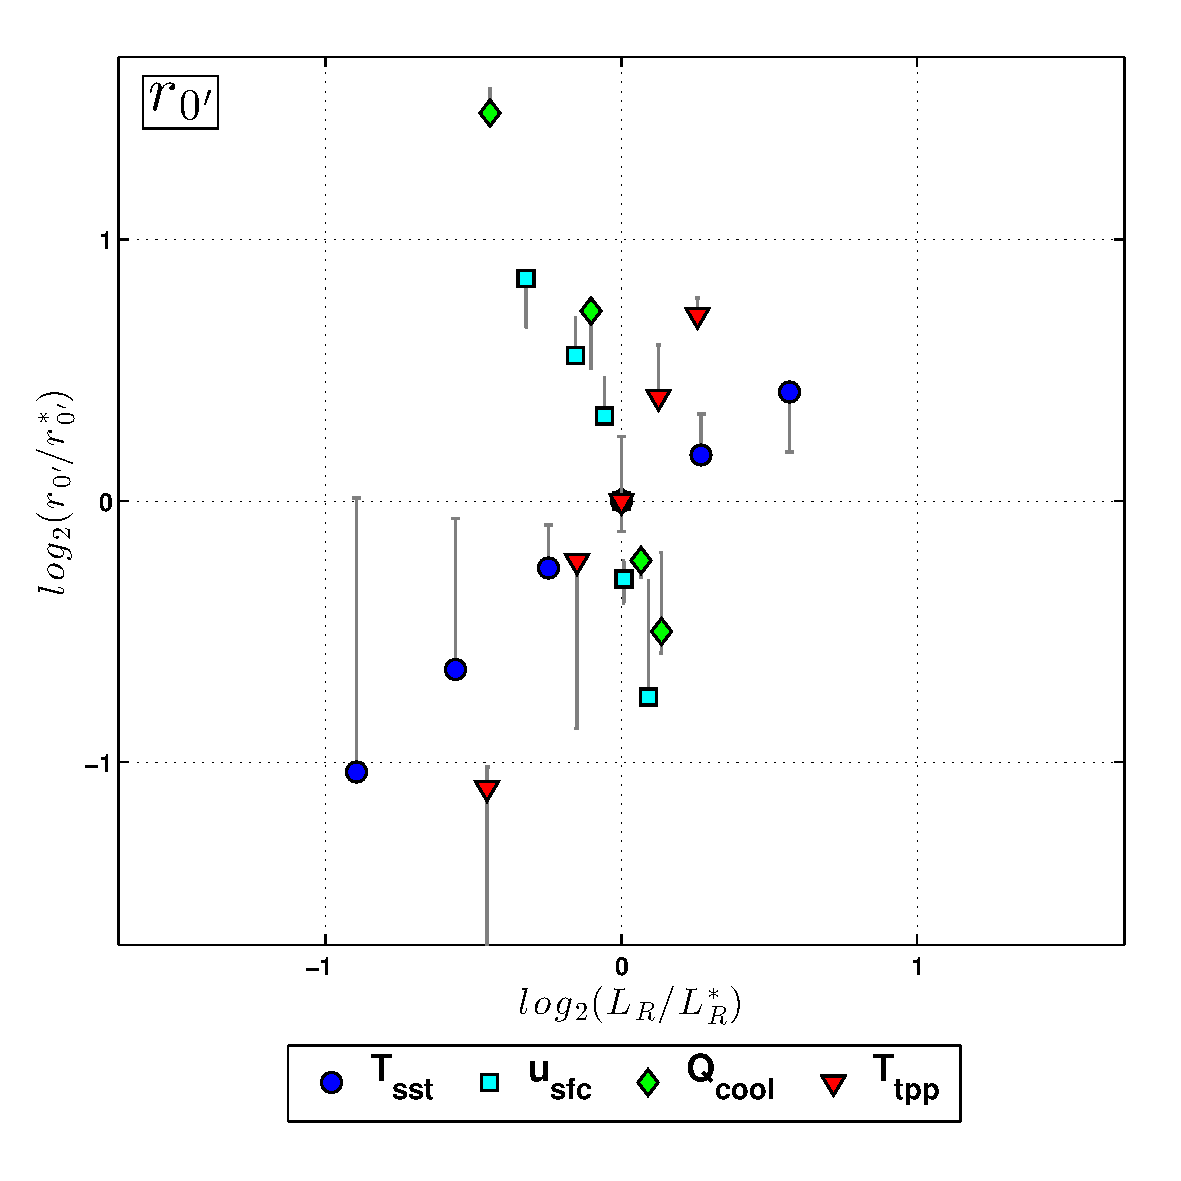
\includegraphics[width=10cm,height=10cm]{FIGURES_TC_RCE_equilibrium_v2.0/Fig5half_LR_nocollapse_r0ctrlwcool.pdf}
\caption{As in Figure \ref{fig:mpicollapse_r0ctrlwcool}, but for the scaling with the Rossby deformation radius.}
\label{fig:LRnocollapse_r0ctrlwcool}
\end{figure}

\begin{figure}[h!]
\centering
%  \noindent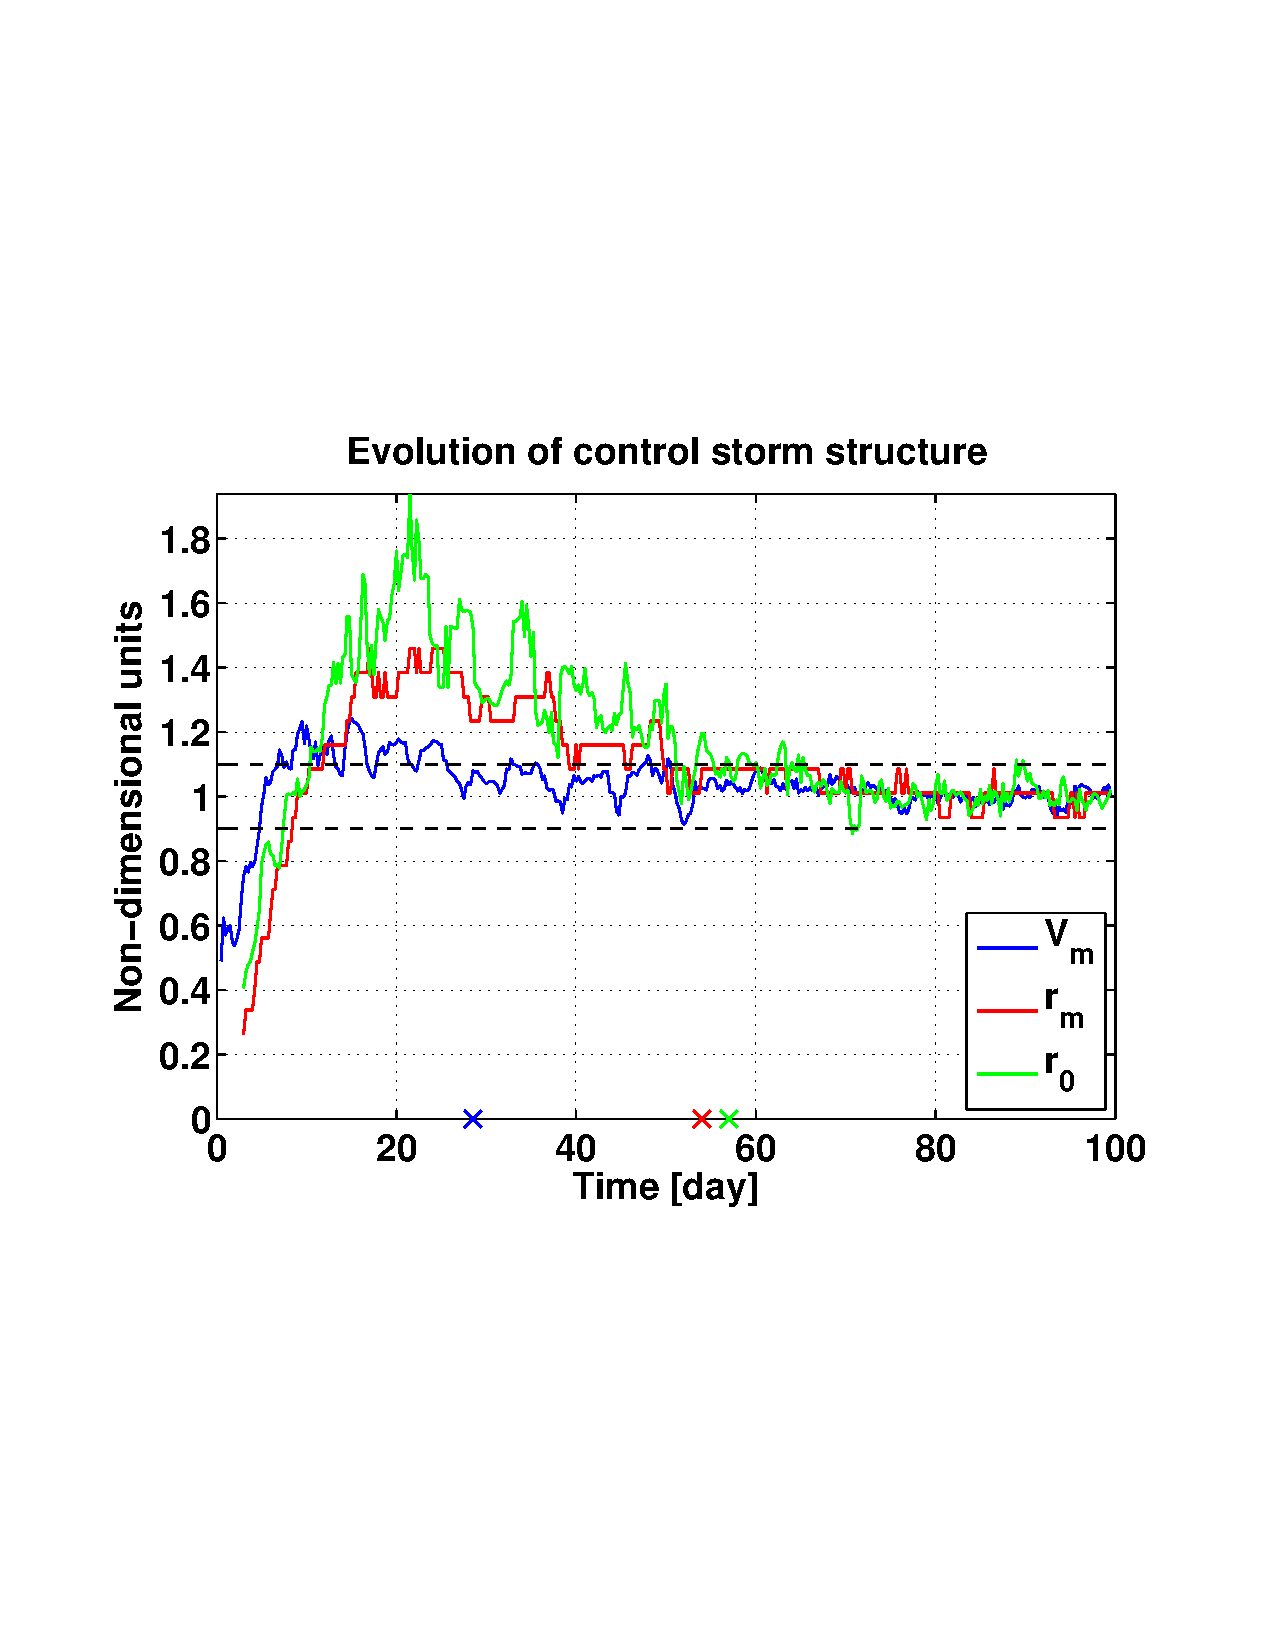
\includegraphics[width=19pc,angle=0]{FIGURES/Control_run.pdf}
  \noindent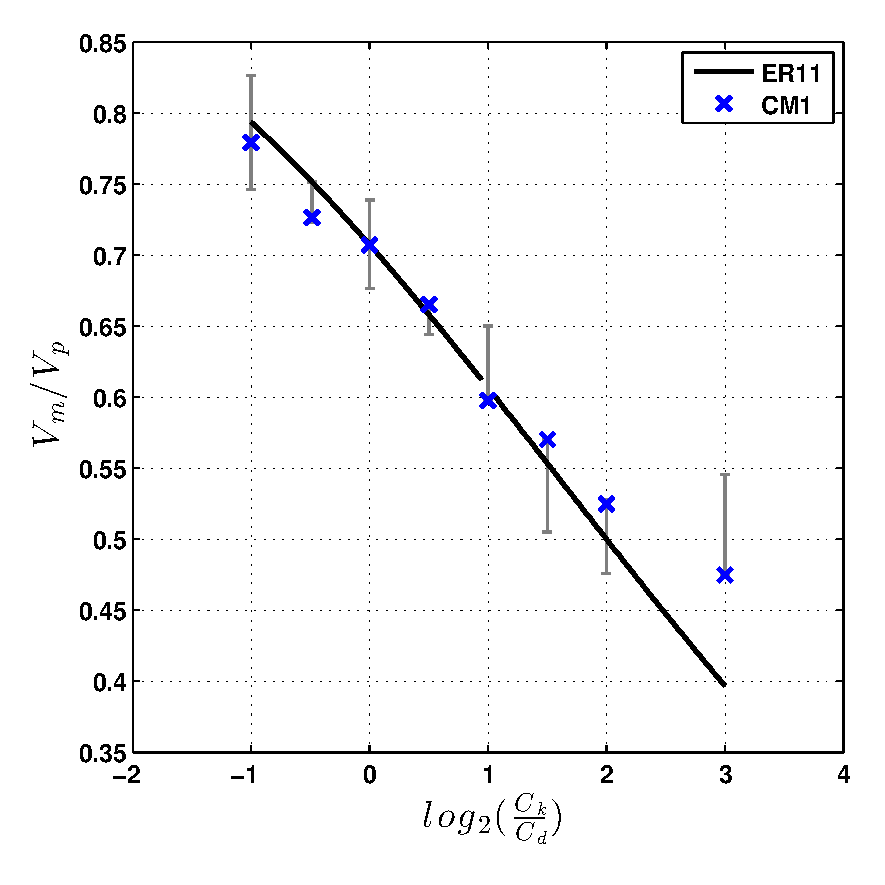
\includegraphics[width=10cm,height=10cm]{FIGURES_TC_RCE_equilibrium_v2.0/Fig9_CkCd_scaling_VmVp.pdf}
\caption{Scaling between $\frac{V_m}{V_p}$ and $\frac{C_k}{C_d}$ in simulations (markers) and the theoretical relation given by \cite{Emanuel_Rotunno_2011}.}
\label{fig:VmVp_CkCd}
\end{figure}


\begin{figure}[h!]
\centering
%  \noindent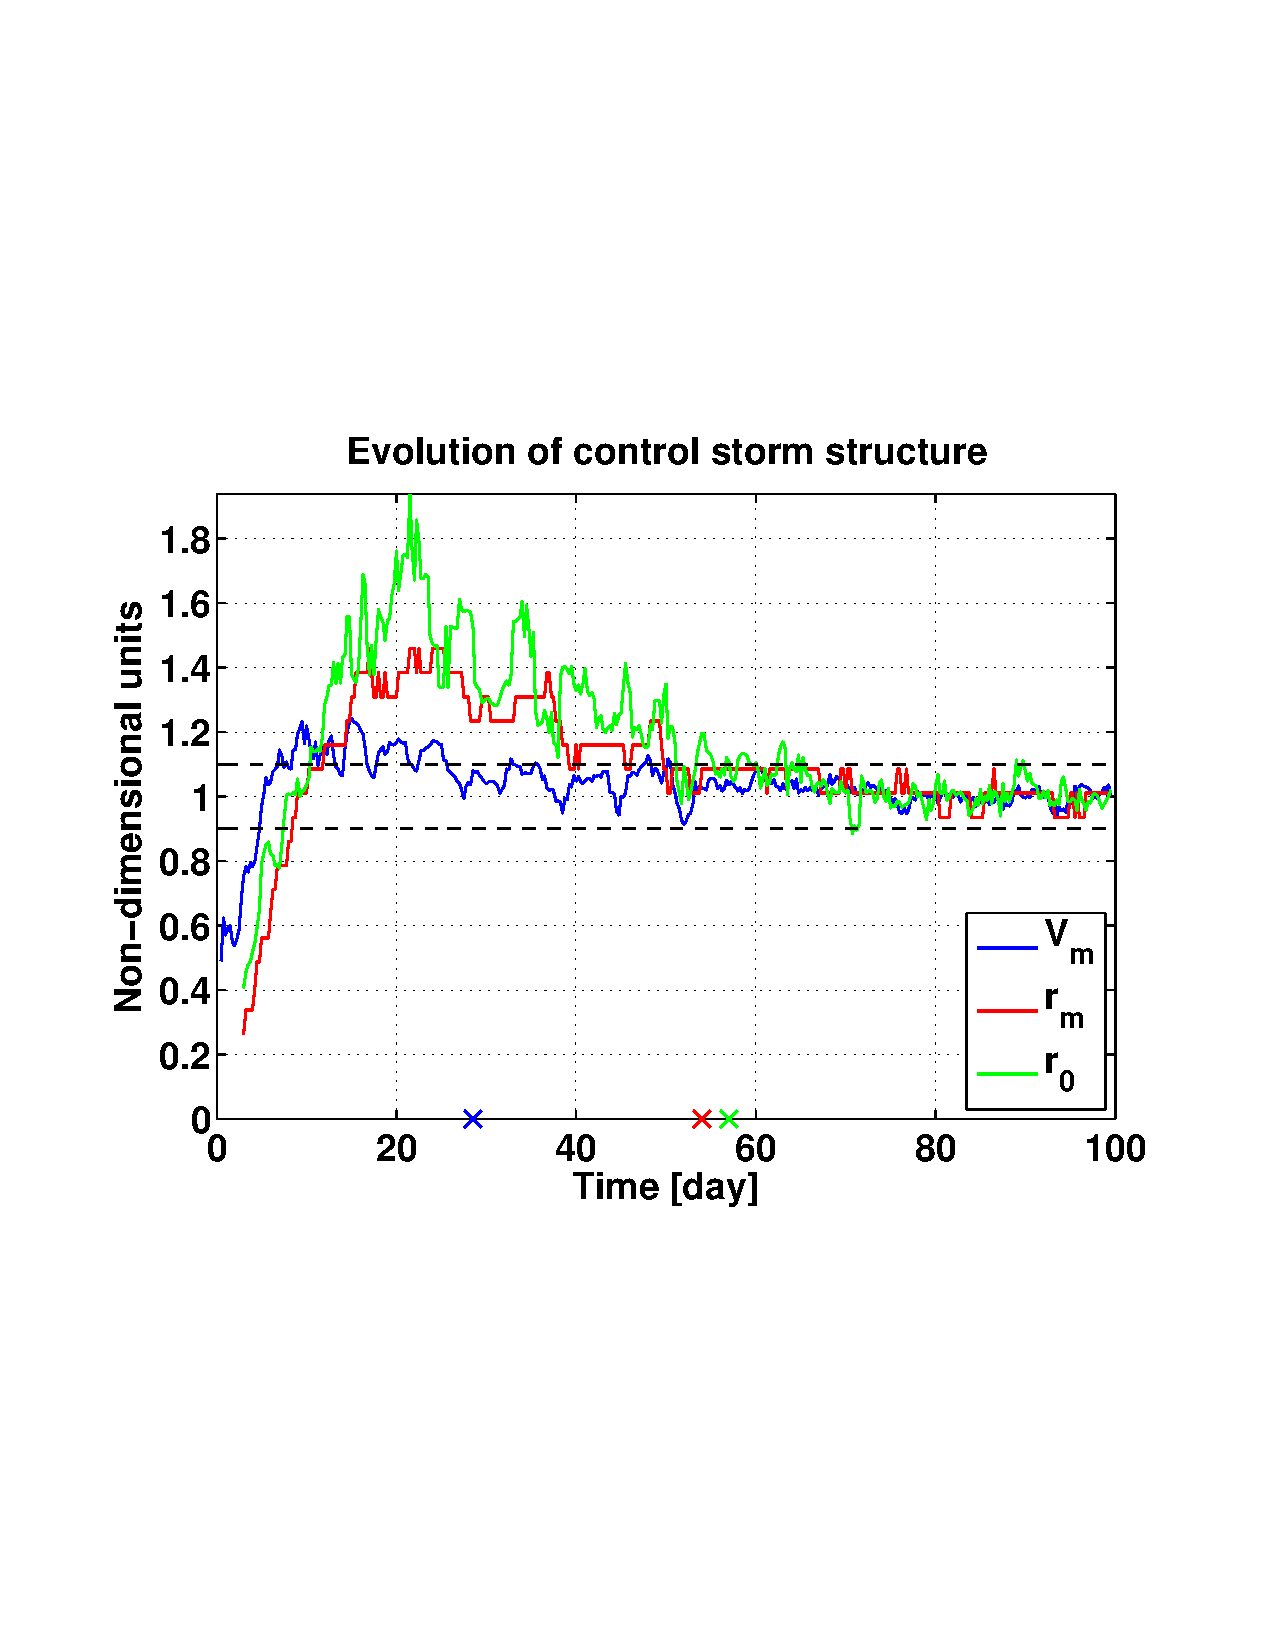
\includegraphics[width=19pc,angle=0]{FIGURES/Control_run.pdf}
%  \noindent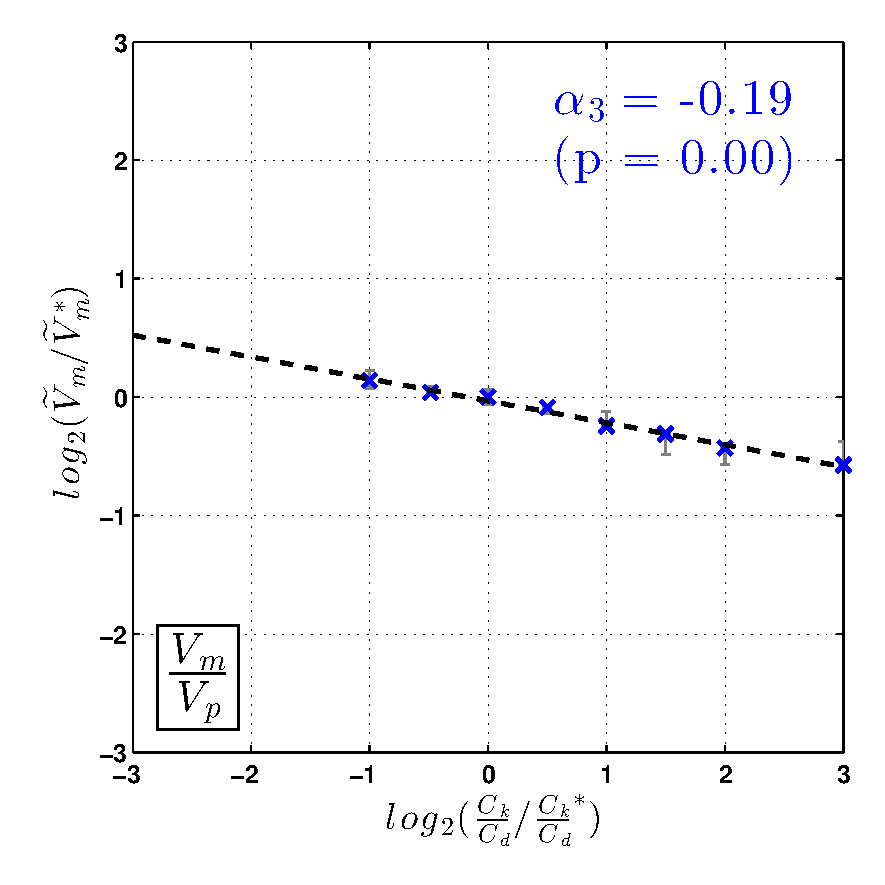
\includegraphics[width=6cm,height=6cm]{FIGURES_TC_RCE_equilibrium_v2.0/Fig8a_CkCd_nondimensional_scaling_V.pdf}
  
  \noindent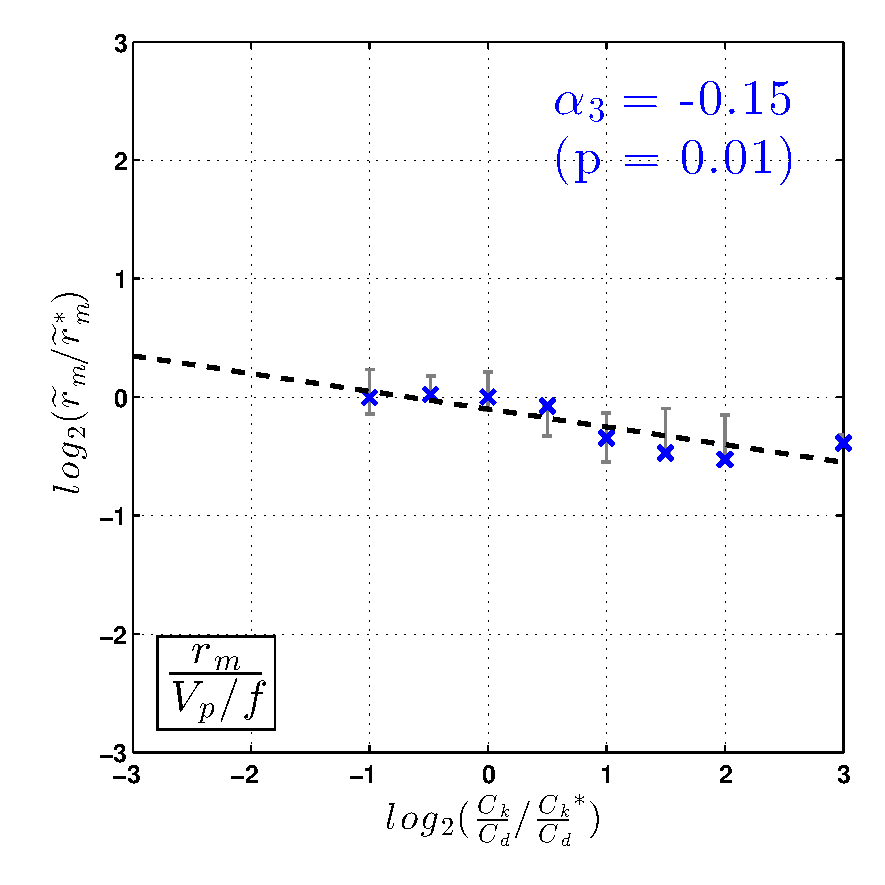
\includegraphics[width=10cm,height=10cm]{FIGURES_TC_RCE_equilibrium_v2.0/Fig8b_CkCd_nondimensional_scaling_rm.pdf}
  
  \noindent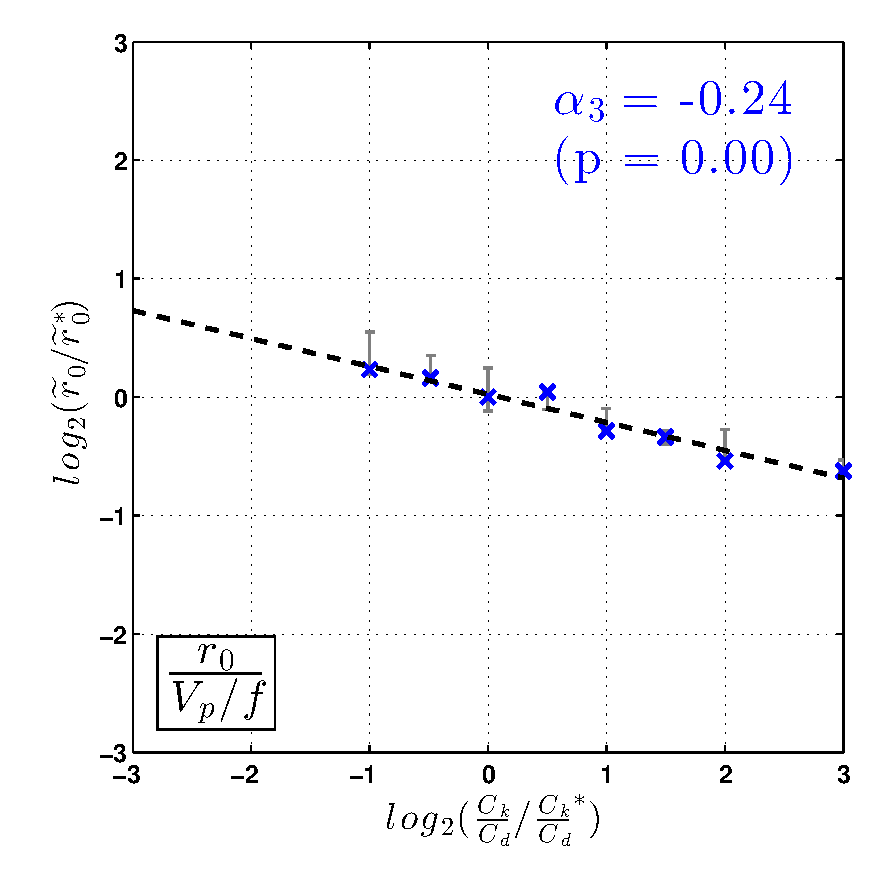
\includegraphics[width=10cm,height=10cm]{FIGURES_TC_RCE_equilibrium_v2.0/Fig8c_CkCd_nondimensional_scaling_r0.pdf}

\caption{Scaling of $r_m$ and $r_0$ with the ratio of exchange coefficients, $\frac{C_k}{C_d}$.}
\label{fig:nondimscaling_CkCd_r}
\end{figure}

\begin{figure}[h!]
\centering
%  \noindent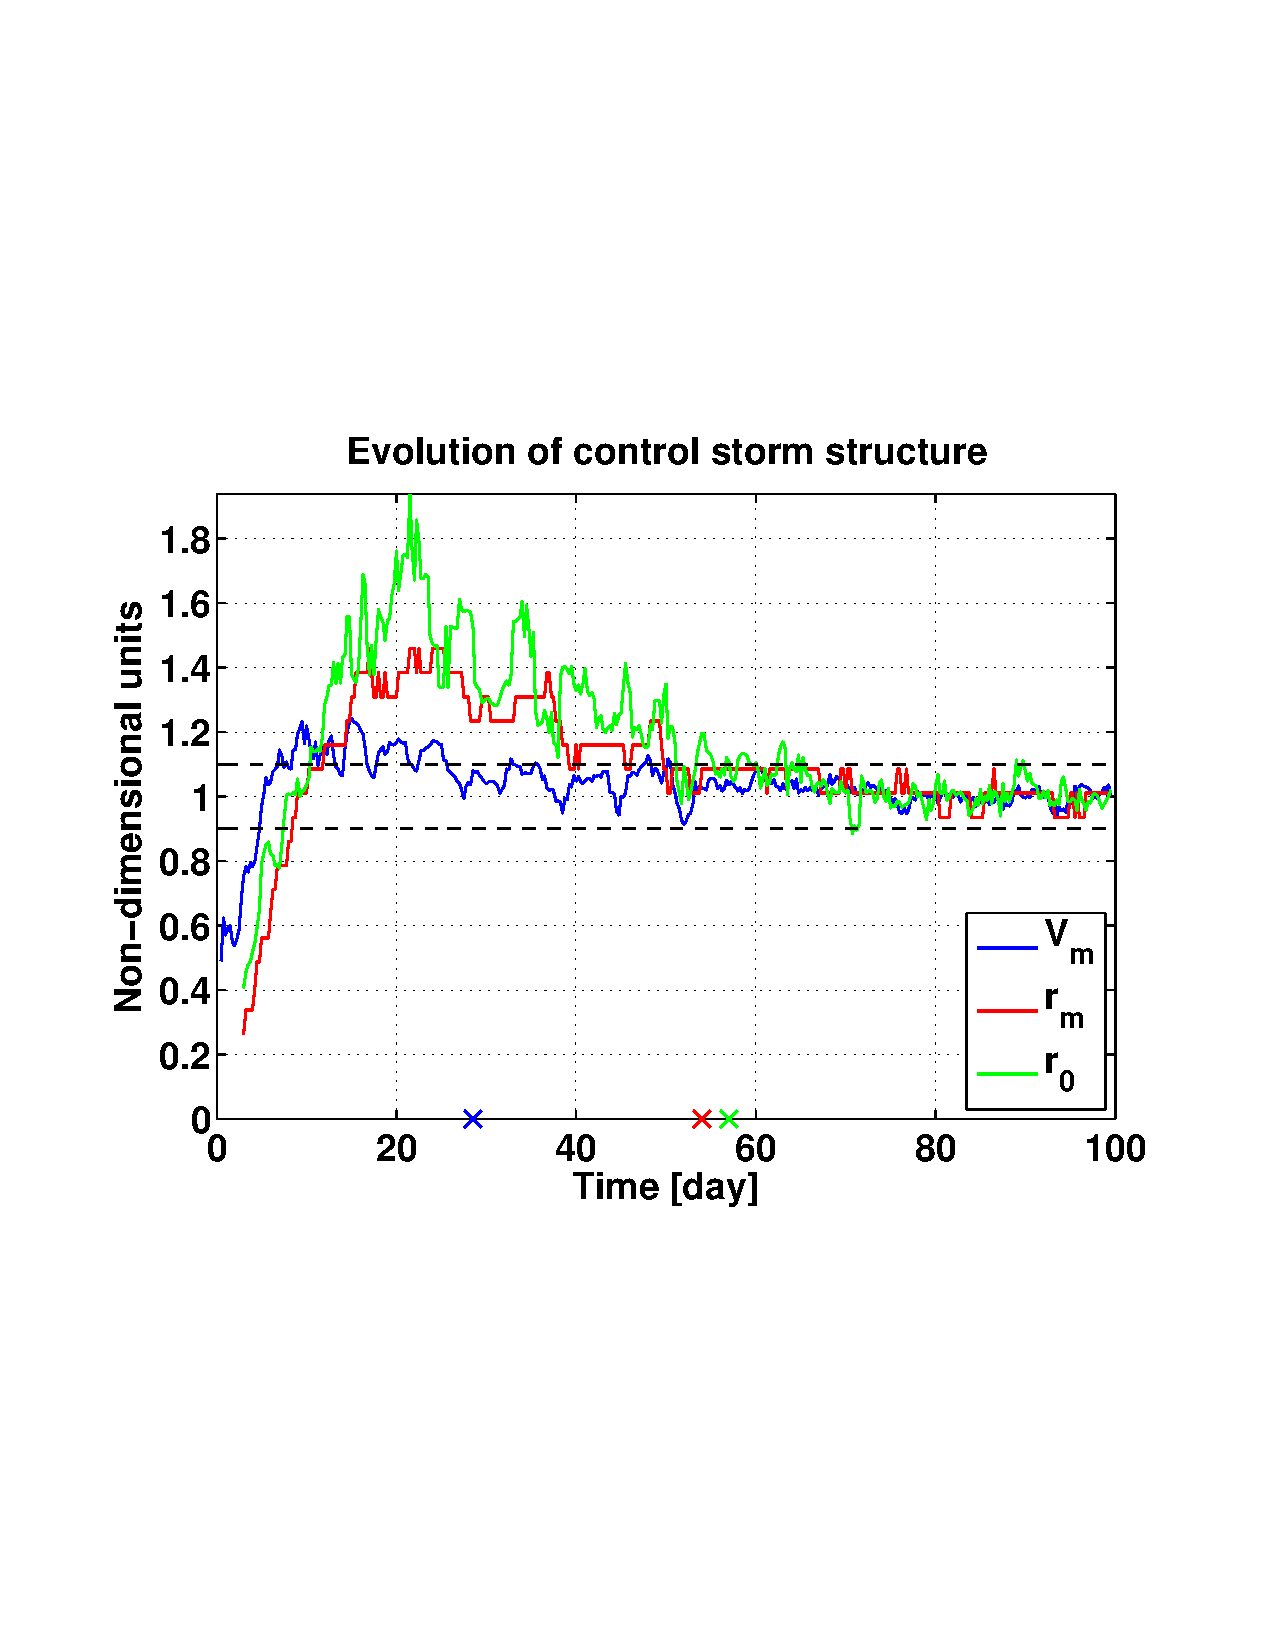
\includegraphics[width=19pc,angle=0]{FIGURES/Control_run.pdf}
  \noindent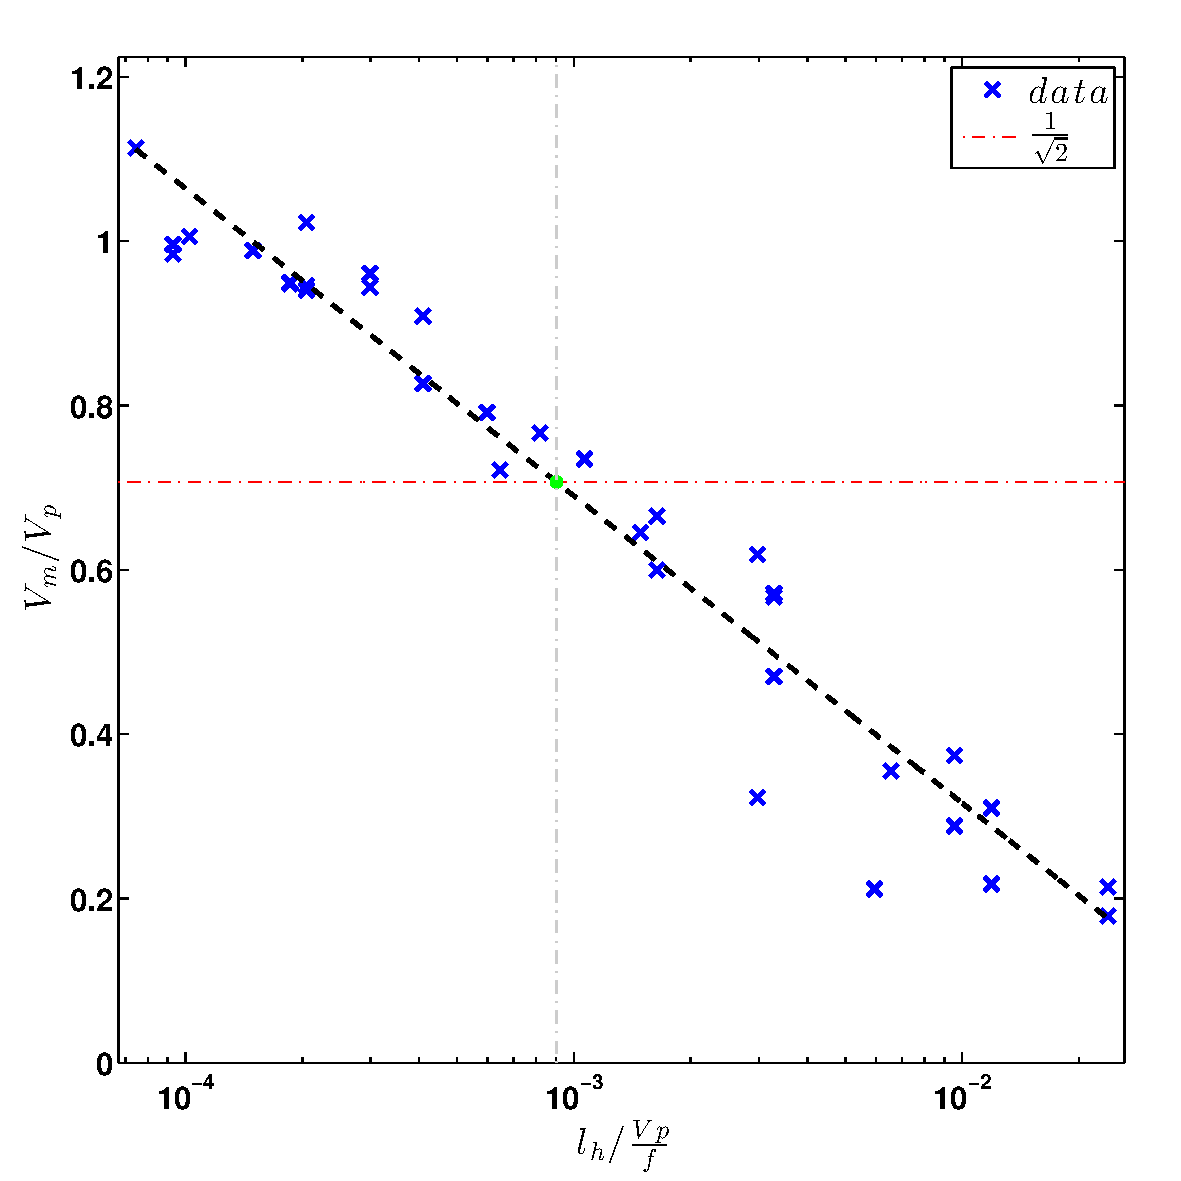
\includegraphics[width=10cm,height=10cm]{FIGURES_TC_RCE_equilibrium_v2.0/Fig10_lh_optimize.pdf}
\caption{Estimation of the optimal value of the radial mixing length normalized by $\frac{V_p}{f}$ by matching the logarithmic fit to the data (black dash) to the theoretical relationship of $\frac{V_m}{V_p} = \frac{1}{\sqrt{2}}$ (red dash-dot) for $\frac{C_k}{C_d} = 1$ in \cite{Emanuel_Rotunno_2011}. The best estimate (green dot) is $l_h / \frac{V_p}{f} = 9.4*10^{-4}$.}
\label{fig:lh_optimize}
\end{figure}

%%SAMPLE
%BEGIN COMMENT
\begin{comment}
\begin{figure}[t]
  \noindent\includegraphics[width=19pc,angle=0]{/Users/drchavas/Documents/LaTeX/AMS_LaTeX/figure01.pdf}\\
  \caption{Enter the caption for your figure here.  Repeat as
  necessary for each of your figures. Create a figures directory and
  place all figures in that directory. Figure from Knutti et al. (2008).}\label{f1}
\end{figure}
%%%%%%%%%%%%%%%%%%%%%%%%%%%%%%%%%%%%%%%%%%%%%%%%%%%%%%%%%%%%%%%%%%%%%
% TABLES
%%%%%%%%%%%%%%%%%%%%%%%%%%%%%%%%%%%%%%%%%%%%%%%%%%%%%%%%%%%%%%%%%%%%%
\begin{table}[t]
\caption{This is a sample table caption and table layout.  Enter as many tables as
  necessary at the end of your manuscript. Table from Lorenz (1963).}\label{t1}
\begin{center}
\begin{tabular}{ccccrrcrc}
\hline\hline
$N$ & $X$ & $Y$ & $Z$\\
\hline
 0000 & 0000 & 0010 & 0000 \\
 0005 & 0004 & 0012 & 0000 \\
 0010 & 0009 & 0020 & 0000 \\
 0015 & 0016 & 0036 & 0002 \\
 0020 & 0030 & 0066 & 0007 \\
 0025 & 0054 & 0115 & 0024 \\
\hline
\end{tabular}
\end{center}
\end{table}
%END COMMENT
\end{comment}

%
\end{document}